\documentclass[a4paper,12pt]{booksfsf}
%\documentclass[a4paper,12pt,twoside,fleqn]{booksfsf}

\usepackage{hyperref}
\usepackage{latexsym}

\usepackage[table,dvipsnames]{xcolor}

\usepackage{graphics}
\usepackage{graphicx}
\graphicspath{ {images/} }

\usepackage{amsmath}
\usepackage{psfrag}   
\usepackage{cite}
\def\citepunct{], [}
\def\citedash{]--[}

\usepackage{pdfpages}                           % To allow inclusion of the frontpage as a pdf-page
\usepackage{caption}   
\usepackage{captspec}
\usepackage[printonlyused]{acronym} 
\usepackage{makeidx} 
\usepackage[english]{babel} 
\makeindex  
\usepackage{color}
\usepackage{tabularx}
\usepackage{amsbsy}
\usepackage{lscape}
\usepackage{breakurl}
\usepackage{appendix}

\usepackage{csquotes}

\usepackage[labelfont = it, font = footnotesize, hangindent = 26pt, parskip = 20pt]{subfig}
\usepackage{enumerate}

\setlength{\oddsidemargin}{0.746cm}
\setlength{\evensidemargin}{-0.1in}
\setlength{\textwidth}{15.5cm}
\setlength{\topmargin}{-0.45in}
\setlength{\headheight}{0.3in}
\setlength{\headsep}{0.35in}
\setlength{\textheight}{24cm}
\setlength{\footskip}{0.4in}

\renewcommand{\baselinestretch}{1.20}
\renewcommand{\captionfont}{\footnotesize\itshape}

\renewcommand\sfdefault{phv}                               % use helvetica for sans serif
\renewcommand\familydefault{\sfdefault}               %    use sans serif by default


\begin{document}

\frontmatter 


\includepdf{frontpage} % Include the frontpage which is a separate pdf. Make sure the pdf exists!
% Note: this only works with PDFlatex. If you use a different typesetter,
% then include the frontpage afterwards, e.g. using Adobe Acrobat

\pagestyle{empty}

%\

%\newpage
%\cleardoublepage

%\chapter{Preface [optional]}
\pagestyle{headings}

The preface is optional. It contains anything that is outside the actual scope of the report, for instance
\begin{itemize}
	\item how you ended up doing the assignment that is reported in this document;
	\item your personal opinion on the subject;
	\item an acknowledgment to the people that helped you carrying out the work.
\end{itemize}
Alternatively an epilogue or acknowledgment chapter could be included in the backmatter of the report.

\chapter{Summary}
\pagestyle{headings}

The following thesis is an account of a research project concerned with the application of version control, a proven paradigm used in software development, to the authoring process of e-learning content. Version control is especially useful in settings of ever-changing text-based data that is created by a large number of people. Therefore, it fits the context of content authoring quite well.

But version control is notoriously hard to use, even for tech-savvy people. For this reason, this project's goal was to develop a simple user interface for version control which could be employed inside a content authoring tool, that is used by a non-technical audience.

The interface design was based on task and requirements analysis as well as insights gained from related research on the usability of version control. During the course of the project the interface went through 3 different design stages. Each iteration of the interface was evaluated by actual users during moderated usability studies. The results informed the evolution of the system and ultimately led to the final design, presented in the end of this thesis.

% please describe main findings in more detail
% high learnability, task completion rate of 82% on average during first time use
% PSSUQ showed that users believe that they could become productive quickly using the system (1.77)
% "I liked using the interface of the system" 1.55
% "The interface of the system was pleasant" 1.66
The research has shown that version control can be vastly simplified and thus benefit a non-technical user-base. The final usability study has shown that the system is intuitive enough to be sufficiently grasped during first-time-usage without prior training (82\% task completion rate on average). Furthermore, users expressed great confidence to "become productive quickly using the system" (1.77 on a scale from 1 to 7, where 1 is strong agreement). Improvements could be made regarding error messages and documentation (Information Quality: 3.31). In general, the user acceptance was high (Overall satisfaction: 2.11), which indicates a positive attitude towards the novel version control features and a likely adoption of the system in the future.

The project's intention is to kick off a discussion on the viability of version control outside the realm of programming and make advanced features, such as merging and diffing, available to a wider audience.

%Topic/Research Question:
%The following thesis investigated how version control, a paradigm known from software development, could improve the creation and management of e-learning content. The research was conducted in cooperation with Babbel, one of the European market leaders in the space of online language learning. The company offers 14 different learn languages, each of them consisting of hundreds of unique lessons. These lessons are created and managed by a group of linguists utilizing a custom content authoring tool. The research question asked whether such an authoring tool could benefit from an integrated version control system.

%The amount of data on the web is rising daily, but the tools used for managing this data have not evolved to meet the increasing requirements. Version control, which is used for large software development projects, is built for ever-changing data and easy collaboration. But the complexity and poor usability of most version control systems have prevented a wider adoption. This project tried to integrate version control and content authoring while laying special focus on usability to make the system attractive to a non-technical audience.

%Methods:
%The design of the system was based on a user and task analysis and was improved iteratively over the course of two usability studies.

%Results/Conclusion:

% Babbel.com, the interactive language learning service, uses a self-made content authoring tool for managing large amounts of data. Creeping featurism has lead to a situation in which usability is at a low point and errors by the user are penalized hard. This project investigates a possible solution to the problem by taking a proven solution from the development world, namely version control, and adapting it for the use by non-technical users through a graphical user interface. The goals being a greater error-tolerance and simplified collaboration between employees.

%The summary consists of one or two pages, and covers all chapters of the report except the appendices. In other words: it should at least summarize the back\-ground/moti\-vation of the work, the goal or research question, the approach, the results, and the main conclusions and recommendations. Divide the summary in paragraphs that roughly correspond to the chapters in the main body of your report. You do not need to explicitly mention the different chapters though.

%Introduce acronyms in your summary \emph{only} if you use them later in the summary. Do not use the \texttt{$\backslash$ac} command in the summary.

%It is not very common to cite references in the summary. It is possible though, particularly if the presented work really builds up on one or more particular papers/reports.

% What is your topic?
% Why is it important?
% What did you do?
% What are your results?



\tableofcontents

\chapter{List of acronyms}

\begin{acronym}[TDMAAA]
    \acro{CAT}{content authoring tool}
    \acro{CLI}{command line interface}
    \acro{DL}{display language}
    \acro{GUI}{graphical user interface}
    \acro{HTA}{hierarchical task analysis}
    \acro{LL}{learn language}
    \acro{MOOCs}{massive open online courses}
    \acro{PM}{project manager}
    \acro{SD}{standard deviation}
    \acro{QA}{quality assurance}
    \acro{VCS}{version control system}
\end{acronym}


\mainmatter

% defining rules for frames around figures
\setlength{\fboxsep}{0pt}
\setlength{\fboxrule}{1pt}

%\chapter{Introduction}
\label{chap:introduction}

Below you find an example of an introduction structure. See \cite{Leferink12,Meijerink12} for more extensive hints on writing.

\section{Motivation}
\label{sec:motivation}
What is the relevance of the presented work, and what is the relation to previous work done in this field?

\section{Framework}
\label{sec:framework}
Where was the presented research carried out, and to what project(s) is it related? 

Possibly this section is combined with the first section, particularly if the presented work is directly motivated by previous work done in the same group. 

\section{Goal(s) of the assignment/Research question(s)}
\label{sec:goal}
What is aimed to be achieved by this work? Or: what is the particular question that is answered by this report? 

This section should be short and very specific. 

Possibly several distinct research questions are formuled as a numbered list, but: the smaller the number of questions, the better. 

\section{Report organization}
\label{sec:organization}
This section describes the structure of the report. It consists of one paragraph, listing the \emph{purposes} of the individual chapters (and nothing else), for instance: 

The remainder of this report is organized as follows. In Chapter~\ref{chap:body}, blabla .... Then, in Chapter~YY, ... Finally, in Chapter~\ref{chap:conclusions}, conclusions and recommendations are given.

Note that appendices are not described here, and that the word 'Chapter' is capitalized when it is followed by a number.

The chosen structure should either be a common one, or follow from the foregoing sections in an obvious way. If necessary, one might consider adding one more section between the goal and report organization, describing the rough approach.


\section{Technical level of the introduction}

The introduction chapter should not be too technical, i.e. equations, graphs, and technical drawings should preferably be postponed to later chapters, unless they directly form the core motivation of the work. The technical level of the introduction should be such that the relevance, goal, and logic of the report structure are clear. Possibly refer to later chapters for technical details, in order to reassure the reader.


%\chapter{Body of the thesis}
\label{chap:body}

This chapter contains a few general hints on the writing. See \cite{Leferink12,Meijerink12} for more details.

\section{Structure}
\label{sec:structure}

All chapters in between the introduction and the conclusions serve as a support for what is claimed in the conclusion. Several structures are possible, depending on the type of work. Discuss the structure of your report with your advisor before you start writing the chapters.

When a chapter consists of several sections, introduce the structure of the chapter in the initial section (which could be an unnumbered section). The particular purpose of the chapter should be introduced there as well (as is done above). In case of a comprehensive chapter, end it with a summary or conclusion.

\section{Figures and tables}
\label{sec:figures}
Use figures and/or tables only if this enhances the understanding of the reader. Refer to figures and tables using figure/table environments and labels, resulting in a combination of the chapter and figure/table number (for instance 'Figure~\ref{fig_empty}'), and indicate their purpose; otherwise the figure/table might as well be left out.  

A figure can for instance be a graph, picture, or schematic drawing. Make sure that all relevant aspects of a figure are well visible, when printed on A4 paper. Preferably use vector-oriented graphics, and minimize the use of colors, unless they can be clearly distinguished when printed to black and white.

Captions should be put below each figure, whereas they should be put \emph{above} tables. The captions should only describe what is depicted by a figure/table ('Measured attenuation as a function of frequency for cable lengths of 1~m, 5~m, and 10~m'), and not what should be concluded from it ('The longest cable has the largest attenuation for all frequencies.'). The latter should be put in the refering text. Always try to place the figure/table after the text in which it is refered, preferably at the top of bottom of a page, or in between paragraphs. Related figures can be combined in one figure environment using subfigures. 

If a figure has been copied from a different source, clearly indicate that in the caption (and ask for permission, if required). 

\begin{figure}
%Insert your figure here. Make sure that the type of figure file (eps/pdf/...) complies with your typesetter.
\caption{Empty figure}\label{fig_empty}
\end{figure}

\section{Equations}
\label{sec:equation}
Very short equations such as $I=V/R$ can be created in-line using dollar symbols; otherwise an equation environment (or related environment such as multline or align) should be used. Equations should be numbered after their last line in order to enable referencing elsewhere in the text. Equations are part of the sentences and therefore usually end with a period or comma. For example, according to Ohm's law, the current~$I$ flowing through a resistor is given by
\begin{equation}
I=\frac{V}{R}\,,
\end{equation}
where $V$ is the applied voltage, and $R$ is the resistance.

See \cite{Meijerink12} for some more guidelines or formating equations.

\section{Acronyms}
\label{sec:acronyms}
Acronyms should be introduced upon their first usage in the main body of the report. For instance once the \ac{FCC} has been introduced, it can be abbreviated to \ac{FCC}.

Introducing, using and listing acronyms is facilitated using the \texttt{Acronym} package and \texttt{$\backslash$ac} command. 

A common misconception is that the constituting words should be capitalized when the corresponding acronym is in capitals, but this is only the case when the abbreviated words form a name, such as the \ac{IEEE}. On the other hand, technical terms such as \ac{UWB} or \ac{OBFN} should not be capitalized, even though their acronyms (\ac{UWB} \ac{OBFN}) are. 

Acronyms always have to be introduced in the main body of the report, even if they have already been introduced in the summary. Therefore it is better to use the \texttt{$\backslash$ac} command only in the main body of the report, and not in the summary.

\section{Citations}
\label{sec:citations}
Use citations if the corresponding book, paper, or report supports a claim that you make in your text, or if it clarifies the context of the work (i.e. what related work have you or other people done). Only list references that are actually cited in the text; the bibliography is not just a list 'for further reading' (although that could be made separately), or a list of documents that you consulted during your work. 

If you literally copy text fragments from a different source, explicitly indicate this using quotes and italic characters. Only copy or summarize material from different sources if this contributes to the understanding of the reader; in principle your report should be readable without consulting the references.

The credibility of the claims in your text is largely influenced by the quality of your cited references: for instance papers in international peer-reviewed journals are generally more reliable than Wikipedia articles. 

Also, note that many readers will tend to judge your knowledge on the context of your work based on the references that you cite. 

Some examples are given in the References chapter~\cite{TEwebsite,Cox04,Meijerink05,Meijerink10,Meijerink06,Leferink12,Meijerink12}.

%\include{chap_...}

%\chapter{Conclusions and recommendations}
\label{chap:conclusions}
This chapter consists of two sections.
\section{Conclusions}
The conclusions should directly answer the research question that was formulated in Chapter~\ref{chap:introduction}, or state to what extent the research goal has been achieved. This is what distinguishes the conclusion from the summary: it should \emph{not} summarize the \emph{contents} of the preceding chapters, but rather only what should be \emph{concluded} from them. 

Dedicate one paragraph to each seperate conclusion.

\section{Recommendations}
The recommendations basically answer two questions:
\begin{enumerate}
\item How could the presentated research be improved if it were repeated?
\item What would be the appropriate question(s) for future research starting from what is presented here?  
\end{enumerate} 
Dedicate one paragraph to each seperate recommendation, and clearly distinguish between the two types of recommendations.

\chapter{Introduction}
The emergence of \ac{MOOCs} has spawned a sharp growth in the e-learning industry in recent years \cite{_e-learning_2014}. In 2012, as much as one third of all enrollments in the US were registrations for online courses \cite{allen_grade_2014}. In addition, 77\% of US companies offer advanced professional training based on e-learning to their employees \cite{vernau_corporate_2014}. But it is not just professional or academic education that has driven the growth of e-learning. More and more people are turning to online courses for pursuing personal interests as well. One area that is particularly popular in this regard is online language learning \cite{blake_current_2011,_its_2014}.
% write about how many people use online language learning, how big is the market

% source for "pursuing personal interests"?

%This research project looks at one of these tools and how to improve it, which is used by the European market leader in online language learning, Babbel \cite{_learning_????}.

The increasing popularity of online learning has also increased the demands on content creators and their tools. The systems that have been quietly powering most e-learning platforms are mostly invisible to its end-users. They are often referred to as \textit{learning management systems} or \textit{authoring systems} or \textit{tools} and have vastly simplified the creation, management and distribution of educational material. Some systems even track the learning progress and gather detailed usage statistics thereby allowing educators to optimize the learning content iteratively. But, with the complexity of learning content and number of contributors increasing quickly, these systems also run into limits. Most of these systems were not built to be used by a large number of contributors at the same time. Furthermore, most lack the ability of keeping track of changes made to learning content or to quickly revert changes. These problems together with a growing user base and increasing expectations on e-learning platforms necessitate the development of a new kind of authoring system more sophisticated than its predecessors.

This thesis investigates how language learning content could be created and managed more easily by applying a proven paradigm from the realm of software development, called version control, to a \ac{CAT} used at one of the European market leaders in the space of online language learning, called Babbel. Special emphasis is put on fostering collaboration between different professionals and keeping track of an ever-changing and expanding course structure. The goal is to exploit version control's benefits and make them work for a non-technical user group.

\section{Babbel}
Babbel is a company offering interactive language courses online. It was founded in 2007 and employs about 350 people as of Fall 2015. Babbel users can choose one of 14 different languages to learn. Each course is created uniquely for one language combination, which consists of a user's native language, called \ac{DL}, and the language he or she wants to learn, called \ac{LL}. Education experts, linguists and language teachers working for Babbel are responsible for managing and improving existing courses as well as creating new ones. All courses can be accessed on the desktop as well as on iOS and Android devices. A speech recognition system helps users to practice their pronunciation. The service is subscription-based and customers can choose among 1- to 12-month payment plans\footnote{http://www.babbel.com/prices}.

The research described in this thesis was conducted over the course of almost one year at the Babbel headquarters in Berlin. The author was part of a four-member team and responsible for user research and interaction design. The team was created as part of an effort to completely rethink the way language lessons were authored and maintained at Babbel. One particular aspect of this process, the collaboration between authors, translators and quality assurance professionals, was the main research theme of this thesis, which is described in more detail below.

\section{Motivation} % problem description
With the accelerating adoption of e-learning and rising demands in regards to the user experience of e-learning platforms, the pressure on content creators to deliver high-quality learning content is increasing steadily. But, in order to deliver content that meets these expectations, authoring tools are needed that facilitate collaboration and quality assurance. It seems that many authoring tools were built under the assumption that creating new learning content is a mostly solitary task. But today, especially at Babbel, this is no longer the case. To create a new language course a number of experts are needed. Until a new course is released, there are at least 10-15 individuals who have participated in the production of the course, often even more. The authoring tool currently used at Babbel does not facilitate this workflow very well and has a couple of inherent problems:

% above: source for 'built under the assumption'?

\begin{itemize}
  \item \textit{Collaboration is inconvenient:} Concurrent editing is almost impossible and content needs to be partially locked so that contributors do not interfere with each other.
  \item \textit{Reverting changes is difficult:} A change, after it was saved, cannot be easily reverted. Instead it needs to be undone manually.
  \item \textit{Changes are not tracked:} The system is more or less blind to what was changed, by whom and when. There is no history, which would allow inspecting past changes.
  \item \textit{Quality assurance:} Because changes are not tracked, \ac{QA} professionals need to do more work than necessary, just because they do not know what has changed exactly. Sometimes new content is also overlooked because of that.
\end{itemize}


\section{Research Questions} % Version Control/Proposed Solution/
The problems described above have one commonality: they are not exclusive to content authoring, but frequently occur during large software development projects as well. Most developers mitigate these problems by using a \ac{VCS}. Initially, version control adds a small overhead to the software development workflow, but this usually pays off when projects become more complex \cite{spinellis_version_2005}.

Despite its obvious benefits, version control has not been widely adopted outside of the programming realm. This could be partially due to its usability issues \cite{church_case_2014,perez_de_rosso_whats_2013}.
In the context of this thesis it was investigated if and how authoring tools could benefit from incorporating version control and how such a system could be made more user-friendly. The research question, as already defined in the research proposal \cite{kreiser_master_2015}, reads as follows:

\begin{center}
% original research question from the proposal
%\textit{What is the best way of exposing version control features to a non-technical user-group in the context of a content authoring tool?}
% Can version control be integrated into authoring tools
 \textit{How can version control improve the authoring process for e-learning content?}
\end{center}

\noindent %The next paragraph is not indented
The research question can be further divided into several sub-questions:

\begin{enumerate}
  \item Which features can be simplified or omitted while  preserving the usefulness of version control?
  %\item How can the interaction design address the diverse needs of different users?
  %\item How can a compromise be found between efficiency and learnability?
  %\item How can the weak learnability of VCSs be improved in order to make the interaction more pleasing for inexperienced users?
  \item How can the learnability of VCSs be improved in order to make them more attractive to a non-technical audience?
  \item How can the overhead, usually introduced through a version control system, be reduced?
\end{enumerate}

\section{Methodology}
In order to answer the research question stated above a rather practical approach was adopted. The interface for a new content authoring tool was conceived and turned into prototypes, which were then tested with real users. Emphasis was laid on the version control features as well as the usability of the overall system. In general, the research project consisted of two major phases: the analysis phase and the design and prototyping phase.

During the analysis phase a literature review was conducted as well as two additional analyses performed. The literature review examined research concerned with the usability of popular version control software as well as examples where version control was applied outside of the programming realm. The subsequent analyses were mainly centered around the future users of the system and their goals. Therefore, a task analysis and a user requirements analysis were performed. These ensured that user needs and goals were properly addressed during the subsequent design phase.

Based on the insights gained during the first phase a prototype was designed that incorporated the most important version control features needed for content authoring. The prototype was semi-interactive and tested with 5 users during a task-based usability study. This first study was followed by a focus group meeting during which users discussed the problems they encountered. The focus group put special emphasis on the version control terminology since finding alternatives to the technical and abstract terms used in most version control systems was a key factor for improving the usability of the interface.

The results of the focus group and the first usability study were then used to design an improved version of the interface, which was tested again during a final usability study. The findings informed the final design of the authoring tool and additionally helped to answer the research question described above.


\section{Thesis Structure}
The next chapter (Chapter \ref{chapter:version-control}) will introduce the reader to version control software in more detail. Afterwards, Chapter \ref{chapter:related-work}, introduces the reader to relevant research in adjacent fields. This is followed by a more in-depth description of the user groups and the tasks that constitute the content authoring process in Chapter \ref{chapter:user-research}.
% maybe the user groups need to be further specified? first time they are mentioned in the thesis

In the second half of the thesis the design process as well as the usability tests are covered. Chapter \ref{chapter:first-iteration} is about the first prototype and the first round of user tests. This is followed by a description of the focus group (Chapter \ref{chapter:focus-group}) and the second design iteration (Chapter \ref{chapter:second-iteration}).

Readers who are mostly interested in the outcome of the design phase and the research results can refer to Chapters \ref{chapter:final-design} and \ref{chapter:results-conclusion}. In the last chapter (Chapter \ref{chapter:future-work}) recommendations and suggestions for future research are made.



% long-term goals?

% content at babbel is complex due to 14 times 7 unique combinations
% on average each language offers 100 courses, and more than 1000 lesson (check numbers again)
% tool needs to be powerful, current tool is highly error-prone
% content creation has many similarities to software development (many collaborators, need for high-quality , peer reviews, continously changing content)




%collaboratively by a number of professionals producing the learning material.





%The growth in e-learning is made possible by learning management systems (LMSs) that have automated or vastly simplified the creation of educational material. With the growing user base and increasing demands on e-learning these systems also need to become better.







%This thesis will look at the systems that power the growth of e-learning, almost unnoticed, by most of its users.
%be concerned with the systems behind many e-learning services. Depending on their purpose they are referred to as learning management systems,  or authoring systems.






%not purely professional, many people also learn out of a personal interest in a particular subject matter (citation).




%This is not just done for professional reasons, but also out of personal interest (citation).


%Subjects, that traditionally have been taught by universities only can now be studied by everyone in a self-paced manner. The surge in e-learning offerings has led to a significant reduction in time and resources needed to acquire new skills.



%One area where this is especially true is learning new languages.



% 1. paragraph: growth of e-learning in recent years
% 2. paragraph: authoring systems
% 3. paragraph: thesis topic
% 4. paragraph:









%Ever more people are drawn to self-paced learning online, including a wide variety of subjects.











%Today, more data is generated than ever before in human history \cite{gantz_digital_2012}. The total volume is expected to double about every two years from now. This will lead to a 50-fold increase in data by 2020 compared to 2010. At the same time only 1\% of this huge pool of data is analyzed. This points to a potential problem: Our tools are failing to keep up with the sheer volume of data.










%During the last two years more data has been generated than in the entire human history prior to that period \cite{_big_????}. Computers and the Internet in particular have made adding and storing information vastly more simple.

%This thesis will look at a very small piece of this data and how it is created and managed at a small startup in Berlin, called Babbel.

%The data Babbel cares about is

%Data itself is meaningless. Especially

%the thesis is about language and data/computers.


%This thesis is about two of the most important human inventions: languages and computers.


%Companies, such as Google or Facebook have built empires based on this data.

%The following thesis is about a very small piece of this data.

%But despite this enormous shift the way data is created and managed has not changed that much.

%This thesis is about a particular kind of data: language.

%To write an ‘eye-catching’ opening sentence that will keep the reader’s attention focused;

%the theme is collaboration on data creation, history of data, compraring data


%Move 1: Establishing a research territory
%- by showing that the general research area is important, central, interesting, problematic, etc. (optional)

%- by introducing and reviewing items of previous research in the area (obligatory)


%Move 2: Establishing a niche
%- by indicating a gap in the previous research or by extending previous knowledge in some way (obligatory)

%Move 3: Occupying the niche
%- by outlining purposes or stating the nature of the present research (obligatory)

%- by listing research questions of hypotheses

%- by announcing principal findings

%- by stating the value of the previous research

%- by indicating the structure of the research paper


%One of the key aspects of writing an introduction, in many disciplines, is to attract the interest of the reader


%To ensure that there is a direct relationship between the introduction and the remainder of the dissertation;
%To ensure that you do not promise what cannot be fulfilled or what goes beyond what can reasonably be expected.

\chapter{Version Control} \label{chapter:version-control}
The following chapter will introduce the reader in more detail to version control systems. A definition is provided as well as a brief introduction into the taxonomy and different concepts of version control. In the end, Git, the VCS most of this thesis is centered around, is explained more precisely.

\section{Definition}
A version control system, also referred to as revision control or source control, tracks changes that are made to a set of documents. The documents and all changes that have been made in the past are stored inside a store called  \textit{repository}. New versions of a document can be added by \textit{committing} changes to the repository. This action creates a unique version number and associates author, time and a short description with the state of the content. This allows users to reverse changes and simplifies collaboration. For these reasons, and because it works well with text-based documents and source code in particular, version control is used heavily within the software development realm.

%Most version control systems have additional features, such as automated \textit{merging} of files as well as \textit{branching}, which allows keeping several parallel versions of a project.
%enables its users to keep different versions of a document. The system records changes that are made to a document, thus allowing users to go back in time and recover older versions. Furthermore, it can simplify collaboration through automated merging of files. Thus, when two people have edited the same file and want to bring their changes together, the system offers a way of doing so.
% A VCS enables developers to keep historical versions of source code and project files that are under development and thereafter to retrieve past versions
% the management of changes to document
%  to keep track of different development versions of source code.
% A version control system (also known as a Revision Control System) is a repository of files, often the files for the source code of computer programs, with monitored access.


\section{Taxonomy and Concepts}
The general concepts and terms described below are mostly shared between different version control software. Nevertheless, no system is like the other and the naming can vary a lot from software to software. For this reason, Git, the most widely adopted version control software \cite{_stack_2015} was chosen as a basis. The features are explained conceptually, so that the reader will be equipped to follow the reasoning of this thesis. For a more technical and detailed description of the inner workings of version control other sources can be consulted \cite{baudis_current_2009} \cite{chacon_pro_2009} \cite{pilato_version_2008}.

\begin{figure}
 \centering
 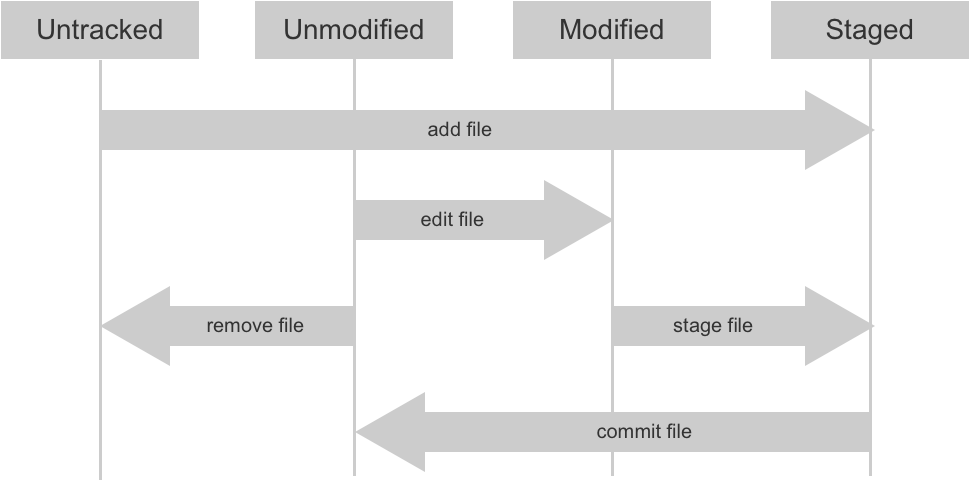
\includegraphics[width=8cm]{version-control/state_of_files}
 \caption{How the state of a file changes}
 \label{fig:file-state}
\end{figure}

%should mention somewhere that his graphic was adopted from the Git Pro book http://git-scm.com/book/en/v2/Git-Basics-Recording-Changes-to-the-Repository

\begin{itemize}
  \item Repository: a database that holds file contents and all versions since creation. A new repository can be created by issuing the \textit{init} command inside a directory. This means that from that moment all files in the directory and its sub-directories can be tracked by version control, unless told otherwise (see next bullet). Repositories can be either local (situated on the client machine) or remote (on the server).
  \item Tracked, untracked and ignored files: when a new repository is created it is empty. It has to be specifically told which files from the working directory should be tracked. This can be done by using the \textit{add} and \textit{commit} commands. If certain files should not be tracked, they can also be ignored permanently.
  \item Working directory: the working directory represents the state of the latest commit of the currently selected branch plus the changes that were made since then. It can also include untracked or ignored files.
  \item Staging area: this is a layer in between working directory and repository. It allows developers to control in a fine-grained way what exactly will be part of the next commit.
  \item Snapshotting: the process of adding a new version to the history of the repository is called snapshotting. It involves adding changes to the staging area (using the add command) and committing these together with a description of what has changed.  Before staging one can also check what has changed compared to the previous version using the \textit{diff} command. The different states a file can be in during its lifecycle are visualized in Figure \ref{fig:file-state}.
  \item Branching: a branch is a named copy of the entire content stored inside the repository. It allows developers to build features without influencing the stable code. Branches can also be utilized to experiment in case one does not know whether a certain direction will lead to the desired solution.
  \item Merging: the opposite of branching, merging brings different versions of the same file back together. Usually this is automated, but sometimes conflicts occur, when both versions have changes in the same line of code.
  \item Pull Request: a pull request is a formalized way of letting collaborators review changes that are part of a particular branch before these changes are merged into another branch (usually the main branch). The feature enforces the best practice of \textit{peer reviews} and simplifies the communication between developers. It is not part of Git itself but was introduced by Github (Figure \ref{fig:github-pr}).
\end{itemize}

Figure \ref{fig:git-workflow} provides an overview of a typical Git workflow. The cycle always starts with branching off the main development line and ends in merging back into it. In between the developer writes code and commits this code in coherent pieces, so that reviewing is made easier for collaborators. The pull request is just a way of formally asking these collaborators to review a particular chunk of code. It is a Github feature and not part of Git itself.

%write about reviewing changes (by other developers)

\begin{figure}[h]
 \centering
 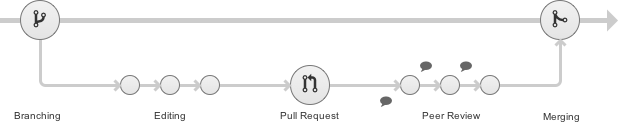
\includegraphics[width=\textwidth]{version-control/git_flow}
 \caption{Version control workflow}
 \label{fig:git-workflow}
\end{figure}


\section{Version Control Software}
The concept of version control is older than some people might think. Early implementations, such as SCCS (Source Code Control System) or RCS (Revision Control System) date back to the 1970s and 80s \cite{_gnu_????} \cite{rochkind_source_1975}. According to Sink \cite{sink_version_2011} version control software evolved in three stages: first generation systems only allowed editing one file at a time that had to be locked while changing it. Second generation systems introduced networking and a central repository for simplifying collaboration. Additionally, the concurrent editing of files was now possible. Apache Subversion, still the second-most popular VCS as of 2015 \cite{_stack_2015}, belongs to this generation. The third generation of version control systems were distributed (instead of centralized), no longer file-based and made branching more convenient. Distributed systems are faster, because the network latency for talking to a central repository is eliminated. Furthermore, third generation systems handle large code-bases more efficiently because these systems do not store copies of each file, but only the changesets. This also makes branching a lot quicker and easier. The most widely used VCS among these third generation systems is Git, which is also described in more detail below.

\section{Git and Github}
Git is an open-source version control software that has its origins in the Linux kernel developer community. After running into licensing issues with a proprietary version control software called BitKeeper, the community developed Git in 2005 in order to replace it \cite{chacon_pro_2009} \cite{ruparelia_history_2010}. The design of Git was based on BitKeeper and the requirements of the Linux developer community. Because it is distributed and changes do not need to be committed to a central repository it is faster than most other VCSs. Furthermore, it supports hundreds of parallel branches and handles large code bases like the Linux kernel efficiently. Git is also workflow agnostic. There is no access management or locking of files. Everyone can edit anything at any time. Conflicts, in case they emerge, are dealt with after the fact, when files are merged together again. As Linus Torvalds said in a presentation in 2007, Git is based on "a network of trust" \cite{_linus_2007}. Companies can decide for themselves what kind of rules or workflows they want to enforce. These characteristics have made Git the most popular VCS in software development by far, beating Subversion as a distant second (69\% vs. 37\% adoption) \cite{_stack_2015}.

\begin{figure}[h!]
 \centering
 \fbox{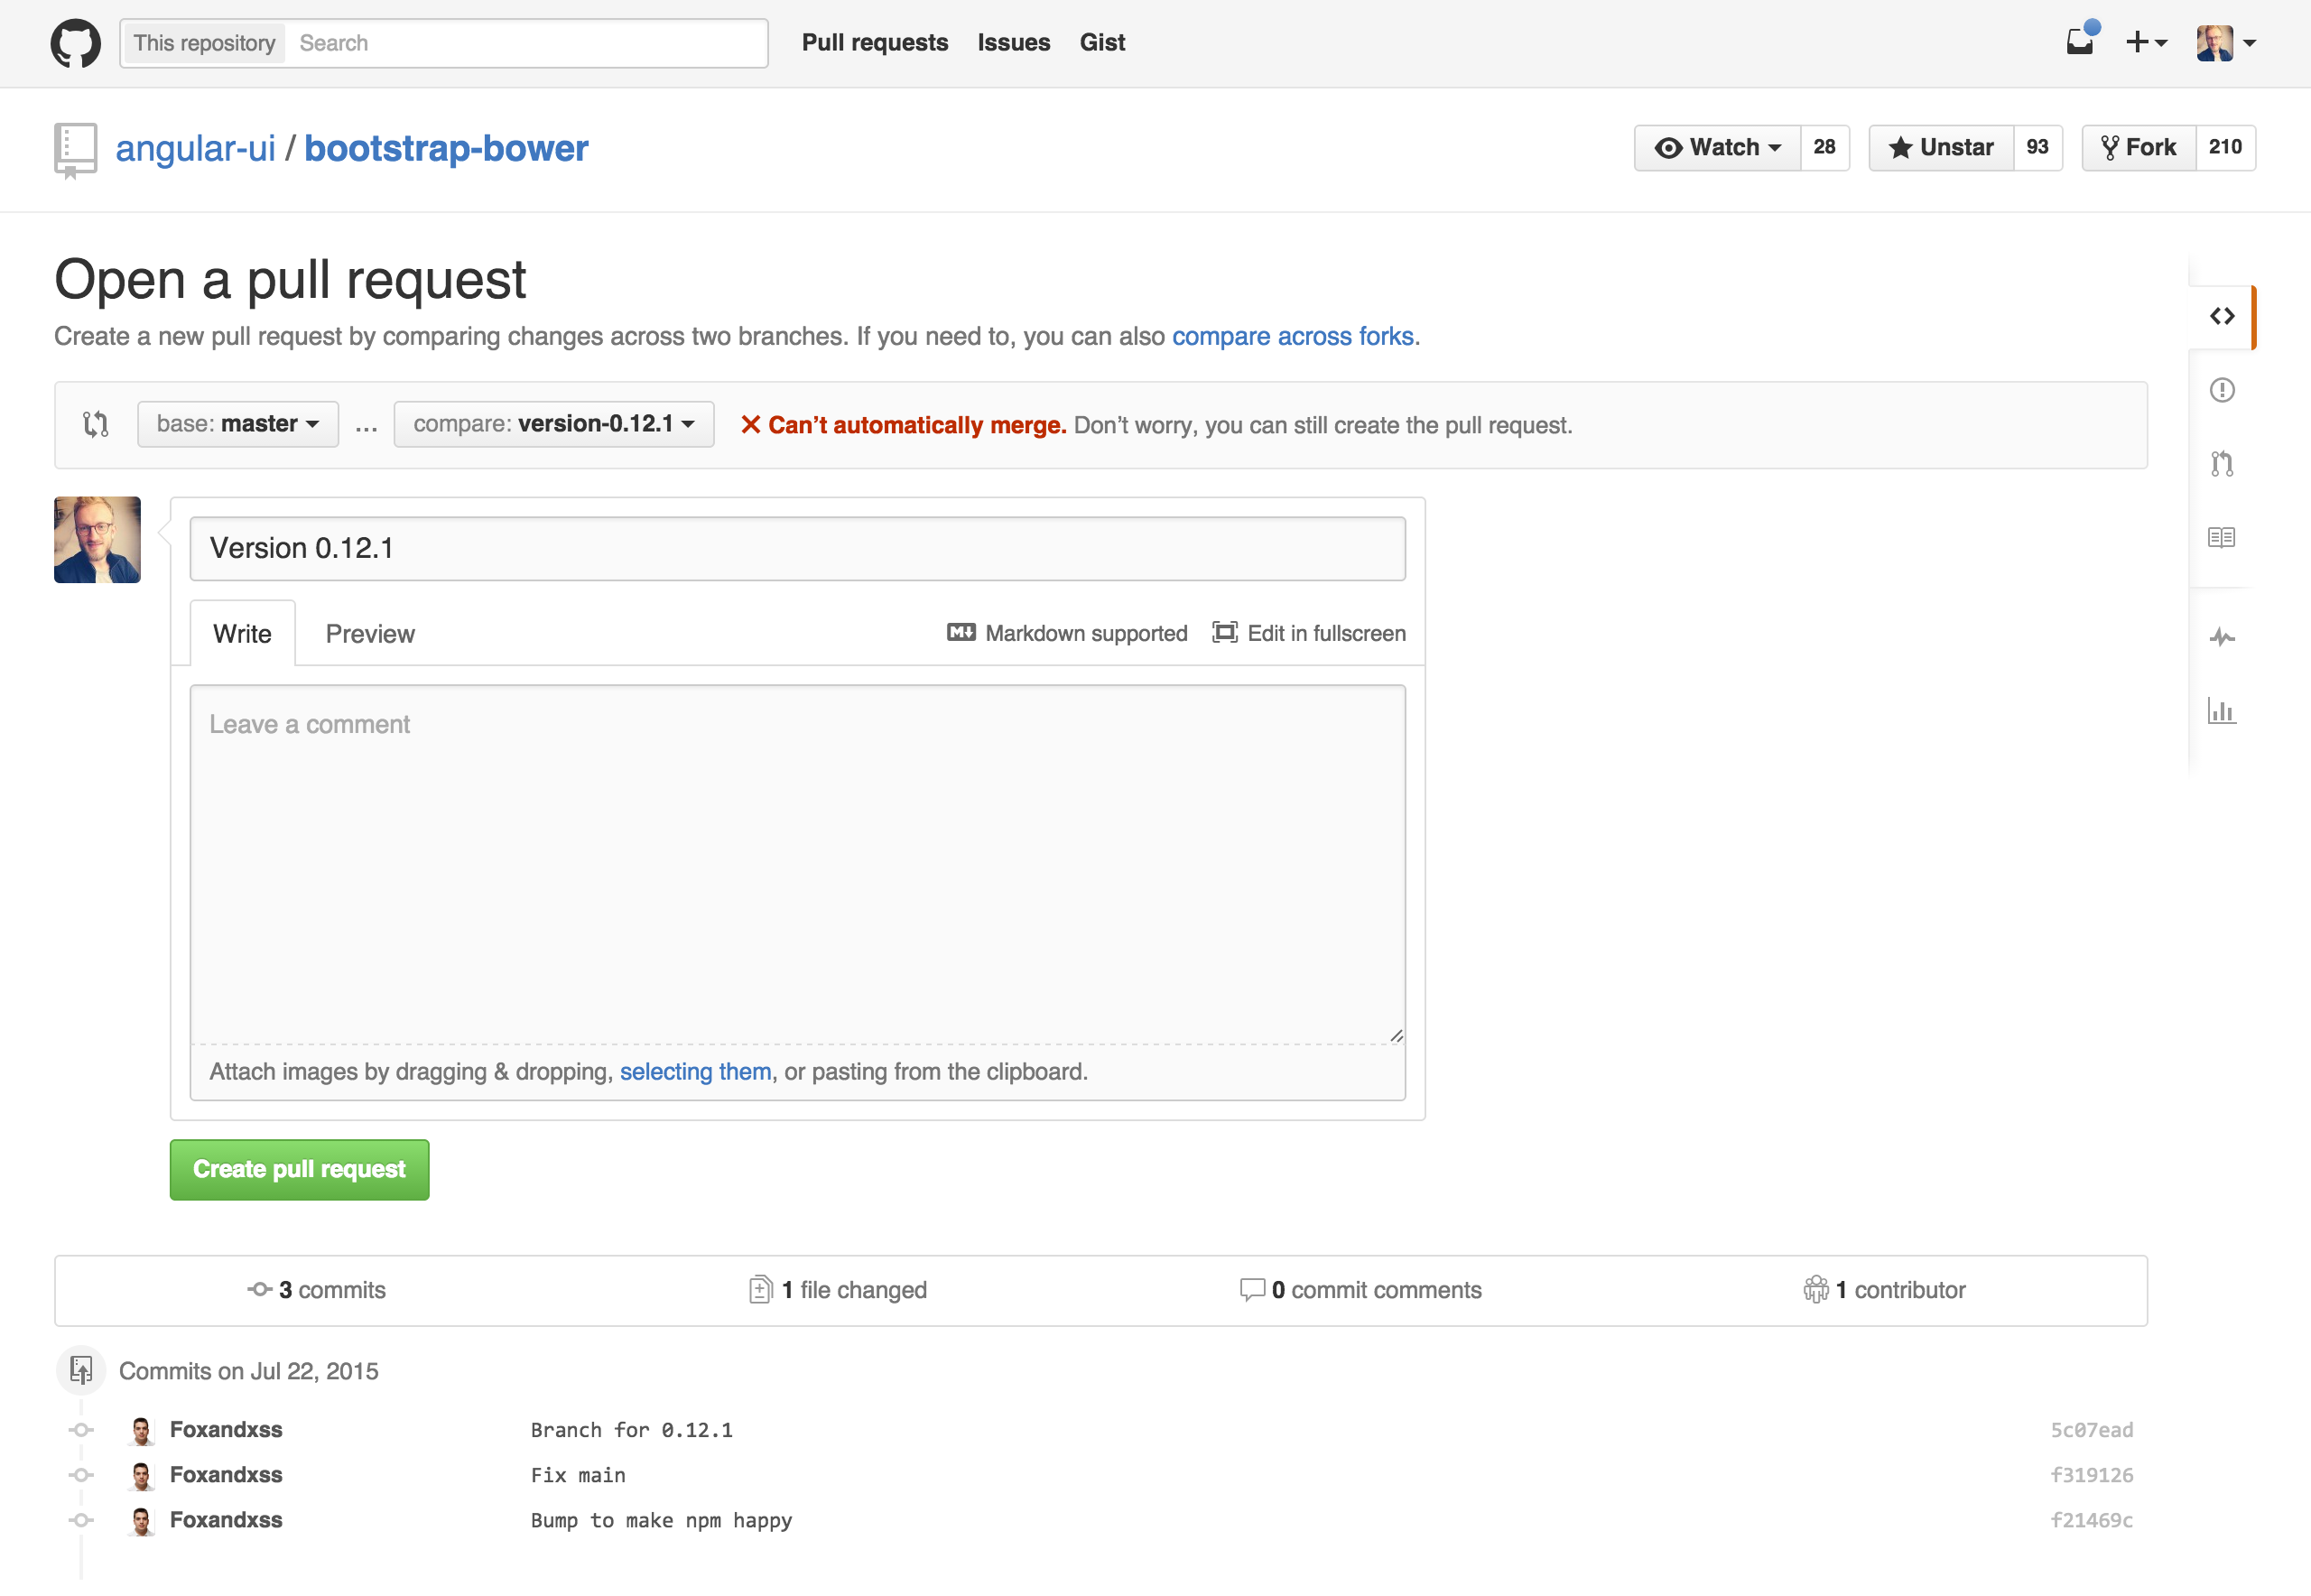
\includegraphics[width=12cm]{version-control/github-pull-request}}
 \caption{Screen for creating a pull request on Github}
 \label{fig:github-pr}
\end{figure}

Github, like the name gives away, is based on Git. It is a repository hosting service that adds additional features, such as access control and social networking capabilities \cite{finley_what_2012}. The service eliminates the need of setting up a personal server in order to host a  repository and makes collaboration simpler by offering wikis, task management and a mechanism for code reviews. All of this is offered through an easy to use graphical user interface. Furthermore, it has become the de-facto standard for sharing open-source projects.

\section{Summary}
Version control software is used to keep track of changing code-bases and for simplifying collaboration among developers. Even though some VCSs have been around for a few decades, the widespread adoption of version control has started only with the second generation of version control systems. Distributed VCSs as well as cloud services, such as Github, have further accelerated this adoption.

Now that the concept of version control is hopefully a little clearer, the next chapter will go on in describing the methodology used for this research project, which will help to ultimately answer the question whether version control can be incorporated into content authoring tools and whether these tools can benefit from it.

% version control is used by a large majority of programmers
% git is the most popular, subversion is second

%\section{Advantages and Disadvantages}
%A version control system allows a developer to keep track of every change that has been made to a source code as well as reversing changes that broke the code. Strangely enough this approach has not made its appearance in a lot of other areas yet. Although Google Docs features a revision history \cite{_google_2010} \cite{30_google_????}, most other software still utilizes simpler means of error-avoidance such as prompts (“Do you really want to delete this file?”) or simple undo actions through the ctrl-z-command. But for systems that handle a lot of data these approaches are very limited and sooner or later users will run into problems (How do I get back to something I changed yesterday?).

%Another reason why developers use version control systems is the simplified collaboration with other developers \cite{spinellis_version_2005}. Before version control, a developer could only edit a piece of code if he or she was sure that no one else was working on it at the same time. Otherwise it would have been nearly impossible to combine the changes that were made by different developers. Most version control systems release the developer from the burden of thinking about this aspect of his or her work. Either through a mechanism called \textit{file locking}, through which the system ensures that only one developer at a time can edit a file, or through something called \textit{automatic merging} \cite{pilato_version_2008}. A functionality that allows changes that were made in the same file to be automatically combined in case there are no overlaps (changes in the same line of the file). This permissive approach usually works well, because even when two developers are working on the same file, they rarely modify the same procedure or module.

%A third advantage of version control, besides easy reversibility and collaboration, is the higher accountability of contributors. Currently, Babbel gives full access to everyone who has the slightest need of accessing the content. This not only includes members of the didactics team, but also people responsible for technical quality assurance or marketing. Everyone can, in theory, manipulate data that effects the live system the end user is exposed to. Because of the suboptimal usability of the system, errors can be introduced accidentally or data can be modified that should not be modified. A version control system makes these changes visible and allows to identify individuals who made changes they were not supposed to do. Currently an employee might never learn that he or she did something wrong.

\chapter{Methods} \label{chapter:methods}
The research project consists of two major phases. Phase 1 is all about analysis: Determining user requirements and finding out what goals these users are trying to achieve by using the software. Phase 2 is about design and user testing. Based on the analyses and the results of the literature study a first prototype is designed and tested. The insights inform the design of the second iteration, which is then tested again in a more thorough way and with more users. This last study not only assures that the implemented changes had a positive impact, but also verifies that all user requirements have been met and that the software allows users to perform all necessary tasks.

\section{Phase 1: Analysis}
The first phase of the project consisted of user research, which established requirements and shed more light on the users' needs. The research served as the basis for designing the first prototype, as described later on, and was also used at the end of the project to determine whether the newly designed software met its purpose. 

\subsection{User Requirements Analysis}
In addition to segmenting the different users into groups requirements were gathered. Since most users are full-time employees at Babbel they were easily accessible. Because of this, requirements were gathered through observational field visits and interviews as proposed by Goodman et al. \cite{goodman_observing_2012}. The observations were particularly fruitful, as users were using an existing content authoring tool already. This helped most of them verbalize what they did not like about it. During the observations the author stayed in the background and only inquired about details of a user's behaviour every now and then. In general, users were left alone and just watched. The field visits were arranged in advance to make sure that users had enough time and were actually using the existing tool at that moment. Each session lasted about 20-30 minutes and was followed by a short interview or open discussion. The author made sure that what he had observed was not based on a wrong understanding and the users could raise concerns or point out especially annoying design flaws. At large, the atmosphere was kept informal so that users could behave natural and did not feel like being part of an artificial situation. The field visits resulted in a long list of requirements phrased as user stories. The stories were composed in a simple structure (see below) as suggested by Cohn \cite{_user_2004}. Terms in angle brackets need to be replaced and square brackets signify an optional section. The stories were ranked by type (functional or quality requirement) and importance. They can be found in Chapter \ref{chapter:user-research}.

\begin{figure}[h!]
\centering

\includegraphics[width=9cm]{user-story-template}
\caption{User Story Template by Mike Cohn}
\label{fig:user-story-template}
\end{figure}

\subsection{Task Analysis}
There are many different ways of analyzing tasks and structuring them in a coherent way. All task analyses are in some way focused on decomposing a task into its constituting parts. The result is often some kind of diagram that visualizes the hierarchy or flow that is inherent to the task. 

For this project, a method called \ac{HTA} was used \cite{hornsby_hierarchical_2010}. It is a simple but effective method for studying work processes and was developed in the 1960s by two psychologists, Annett and Duncan \cite{shepherd_hierarchial_2000}. Their aim was to understand the purpose of work by looking at human activity within organisations and systems. HTA, in the tradition of systems thinking, regards work as a complex system consisting of  interacting sub-systems, which can be machines and humans \cite{shepherd_hierarchial_2000}. These sub-systems interact by means of input and output. The interplay is constantly adjusted through feedback mechanisms, which allow a human operator, to adapt his or her behaviour. 

Based on the analysis, diagrams were created, each of which represents a high-level task that is decomposed into sub-tasks. Each diagram provides an overview of the order in which tasks are performed as well as the mental processes behind them. The diagrams together with a short description of each task can be found in Chapter \ref{chapter:user-research}.

%The complex system examined in this particular case was the process of creating new learning content.

%The HTA described in this section is aimed at identifying tasks that could benefit from the implementation of a version control system. Moreover, the analysis helps visualize how tasks, performed by different user groups, overlap. This could support the design of an interface that facilitates and simplifies collaboration. 

\section{Phase 2: Iterative Design \& Usability Testing}
The second phase consisted of designing and iteratively testing the new interface. The first prototype was based on the insights gained through task and requirements analysis as well as the literature study. It served as a first starting point for discovering usability issues of the version control features of the system.

%This prototype was tested in a scenario-based usability study, which lay focus on the newly designed version control features. 

%maybe mention that research didn't start from scratch - there is other research that has proven version control can be valuable outside of programming - that's why I didn't start with exploratory resarch but with a summative tet 

\subsection{First Study}
% I dont like this paragraph
As a means of detecting usability problems early on the first study was conducted with a semi-interactive prototype that was based on simple graphical layouts. The prototype was mostly black and white and only those parts that were actually needed for the user tests were interactive. This meant that designing the prototype did not take a lot of time and subsequent modifications (i.e. after a design feedback round) could be realized quickly as well. 

The sessions were scenario-based, which means that participants had to perform a number of tasks which reflected their everyday work. This put more emphasis on the actual behaviour of users instead of opinions and attitudes and allowed the test moderator to stay in the background. This method is often referred to as \textit{assessment} or \textit{summative study} \cite{rubin_handbook_2008} \cite{goodman_observing_2012}. These kind of studies can yield more honest results because the method involves less interference than for example exploratory tests. The number of participants was kept rather small, informed by Nielsen's insight that 5 users are sufficient to find 85\% of the usability problems if the user group is somewhat uniform \cite{nielsen_why_2000}. 

Additionally, a few quantitative metrics were taken in order to support the results of the observations. Among them task completion rate, time for task completion and error rate. Because the sample size is somewhat small these metrics can rarely deliver statistically significant results, but they can serve as an indicator of potential problem areas that should be investigated further. How these metrics were measured is described in more detail in Chapter \ref{chapter:first-iteration}. 

% what is said?
% first paragraph:  prototype (needs work)
% second paragraph: type of study
% third paragraph: quantitative metrics
% fourth paragraph: write about the goals of the study?

% talk about kind of users
% which scenarios?
% or is this part of the subsequent chapters?

%This allows the test-moderator to  

%The goal was to eliminate the most severe problems before implementing them.  


%The goal of the first usability study was to detect severe problems before starting to implement any of the features.  

%The prototype was tested with a handful of users to detect usability problems early on. During this first assessment test, described in more detail 

\subsection{Focus Group}
All participants of the first usability study were also part of a subsequent focus group. The group meeting served as a platform for discussing concerns and the impressions regarding the novel version control features that users were exposed to during the testing sessions. Furthermore, the goal was to identify potential stumble stones in regards to the version control terminology. The terminology used by Git and other version control systems is often rather technical and not necessarily self-explanatory. But the aim is to make the system easy to learn for a non-technical user group as well.

% this paragraph was taken from the research proposal!!
Focus groups are particularly suitable for the early stages of a project. They can be an efficient means of gathering feedback in a short time-frame, because they involve more than one user at a time \cite{rubin_handbook_2008} \cite{goodman_observing_2012}. When conducting focus groups researchers need to be aware of the fundamental difference between what people say and what they do. Only because a participant claims that she likes a product, does not mean that she will actually use it \cite{goodman_observing_2012}. Therefore the outcome of the group should be put into perspective and not applied literally. Furthermore, the results of focus groups should be taken with a grain of salt, due to their small sample sizes. Nevertheless, the outcome can serve as a basis for further research \cite{goodman_observing_2012}. 

% this paragraph was taken from the research proposal!!
% maybe this should be rather part of the actual focus group section
%At the start of the focus group the test moderator explained the purpose of the meeting. Then, the participants were introduced to the version control features that will be exposed in the content authoring tool. These are only about five to six major features. Afterwards, the group will have a discussion on each of these features and whether it needs renaming. If the group comes up with more suitable names for  certain features, everyone is asked to write down his favorite terms on a piece of paper and prioritize them. This is done in order to mitigate social influences by people who are good at phrasing their strong opinions \cite{goodman_observing_2012}. At the end of the meeting there should be a list of proposed names for each term that needs to be renamed. The whole focus group session should not last longer than 1 1/2 hours.

\subsection{Second Study}
The second and final usability study was based on a functional web-based prototype. This prototype contained a number of changes that were made as a result of the findings of the first user study and the focus group. Most notably, the main navigation had changed as well as the way content was represented. Furthermore, a series of severe usability issues had been fixed, mostly related to the version control features of the system. On top of that, some of the main features were renamed, which had been identified as problematic during the focus group meeting. \textit{Branches} were now called \textit{working copies} and \textit{pull request} was changed into a more descriptive \textit{merge request}.

The main goal of this study was to verify whether the introduced changes had a positive impact on the user experience. Hence the name verification or validation study \cite{goodman_observing_2012} \cite{rubin_handbook_2008}.
For this reason, the setup of the study was similar to the first study, which made comparing the results easier. The web-based prototype, which covered a lot of functionality, allowed the moderator to stay in the background so that users could freely interact with the system. This proved to be quite successful in that a lot of new issues were found that had not been discovered during the first study.  

Besides validating the changes the study was also aimed at confirming that the user requirements specified during the start of the project were met. This was done by simply observing whether users were able to perform the desired tasks. Furthermore, a post-study usability questionnaire was used that measured the perceived usability of the system. This helped to identify weak spots and potential areas that would need more attention in the future. 

% new prototype / changes
% talk about goals: 
% prove whether changes that have been made were positive. 
% check whether user requirements have been met
% establish standards for the future (PSSUQ)

% short summary of method, verification/validation
% similar tasks to round 1

\section{Summary}
This chapter described the theoretical basis of the methodology used throughout this research project. The design of the user studies and the procedure during the sessions is described in more detail in Chapters \ref{chapter:first-iteration} and \ref{chapter:second-iteration}. The following chapter will introduce the reader to other research that has been done in the field of version control systems, with a special attention to systems applied outside of the programming realm. The remaining project will build upon this insights and the first prototype was heavily influenced by these findings described in the next chapter. 


%The research project will be divided into two major phases. Phase one will be all about the user and finding out who the user actually is and what kind of goals he or she tries to achieve. For this purpose a bunch of popular user-centered design methods will be used, such as personas, task and requirement analyses and a focus group \cite{mao_state_2005}. 
%During the second phase, the insights gained through the different analyses will be used to create meaningful prototypes. The first prototype will be a static representation of the interface, which can be tested in an exploratory study \cite{rubin_handbook_2008}. The idea is to start with a prototype that maps Git's functionality more or less 1:1 and then see which concepts the users are struggling with the most and then find suitable solutions to that during the design of the next prototype. For the first prototype some inspiration will be obtained by existing GUIs for Git \cite{_git_????}.

%The results of the first user tests will inform the design of a second prototype. This prototype will incorporate interface solutions to the problems users encountered during the first user tests. The second prototype will be interactive so that it can be tested with less interference by the moderator. The hope is that a task-based assessment will yield more genuine results than the exploratory study, especially regarding details of the interface and certain micro-interactions.

%Depending on how well the prototype was received during the assessment a third iteration will be done in which flaws that were encountered are eliminated. This prototype will then be tested once again, with more or less the same setup and methodology.

\chapter{Literature Review} \label{chapter:related-work}
The following section describes three different areas within the scientific debate on version control systems: 1. the usability of version control systems, 2. improvements to version control and 3.  implementations of version control outside of the programming realm. The review serves as a foundation for the research described later on and provides the necessary context in which the results of this thesis should be seen. Furthermore, it enables the reader to assess the contribution of this work to the current state of research.

It seems like most research in the area of version control is concerned with the shortcomings of different systems, both in terms of usability and the conceptual design. In some research projects alternative solutions have been investigated, but those are usually situated within the programming realm. Unfortunately, there are not many examples in which version control has been applied to other domains. In general, most research is focused on the widely used open source VCSs Git and Subversion.

The review is structured into the three areas described above. All literature is shortly summarized, compared and set in relation to other work of the field.  % the criteria are very similar to the 3 areas described in the first paragraph

\section{Usability of Version Control Software}
During the 2011 Git User Survey participants were asked which parts of Git needed improvement. A total of 73\% stated that  the user interface needs improvement \cite{_git_2011}. With this in mind, it is surprising how little research there is about the usability of version control systems in general and Git in particular. The two most notable studies have investigated the user experience as well as the conceptual design of different version control systems, among them Git \cite{church_case_2014,perez_de_rosso_whats_2013}.

Church, Söderberg and Elango have conducted an empirical study on the usage of command line-based version control inside two large IT companies (Google \& Autodesk) \cite{church_case_2014}. The study was based on interviews and observations within these companies. Engineers who participated covered a diverse range of job positions and had varying experience. The study results show that common usage patterns emerge when version control systems such as Git or Subversion are incorporated into the software development workflow. In both companies, most engineers stuck to a small set of commands and showed a general risk aversion when using version control. Church et al. note that the observed "ritualistic behaviour" of engineers is usually found among novice computer users and attribute this behaviour to a low user confidence in the version control systems used. They conclude that it is particularly problematic for a tool whose main premise it is to offer "development without fear" to be perceived as risky to use.

Explaining these results, Church et al. present a cognitive dimensions analysis of Git. They point out that there are many \textit{hidden dependencies}, such as between files and branches, local and remote repositories as well as between untracked files and the repository. Moreover, Git has an "abstraction barrier", meaning that certain concepts, i.e. branching, need to be learned, before the system can be used in a meaningful way. The authors reason that a combination of hidden dependencies and abstraction mostly contribute to the aforementioned usability problems. These conceptual issues are also the reason why the \ac{GUI} client by Github \cite{_github_????} only offers a slight improvement in usability. It makes features more discoverable and offers a more visually pleasing interface, but it suffers from the same deficiencies as the command line interface. The authors close by highlighting that the discovered issues need to be solved before version control can take the leap from computer science to a wider audience.

The second study mentioned above, by Jackson and Perez De Rosso, was based on an analysis of Git's conceptual model. The researchers present the weaknesses in Git's conceptual design and propose an improved alternative called Gitless.

They argue that concepts have a strong influence of how users think about an application and therefore conceptual integrity should be an important consideration in software design. By concepts the researchers mean \emph{"the constructs and notions [...] that are invented for the purpose of structuring the functions of the system"} \cite[p.~38]{perez_de_rosso_whats_2013}. Git's concepts were scrutinized based on three main criteria that were defined by Frederick Brooks in the 1970s \cite{brooks_mythical_1995} and which he believed to be central to conceptual integrity. 1. orthogonality – individual concepts should be independent from each other, 2. propriety – a software should only have the essential functions that are needed for its operation, and 3. generality – a function should be applicable in different ways. After formally describing Git's main concepts the researchers go on in explaining which concepts violate these criteria and why. Regarding the first criterion, orthogonality, the researchers point out that Git's different file states, such as modified, staged and committed, are particularly troublesome. Commands that are primarily intended to modify one state, sometimes also affect the other. For example, if a user modifies a file, stages it and then goes on modifying the same file, the command git commit \textit{file} will commit both states of the file (the staged and the unstaged). This happens, even though the commit command typically only effects the staging area, unless told otherwise by a particular flag.
According to the researchers, the staging area also violates the second criterion – propriety. They argue that an intermediate step between editing and committing is rarely useful and that most users just want to commit their changes right away. Although this is possible through an additional flag (commit -a) this approach has some drawbacks as well, e.g. that untracked files will not be included in the commit and that a high verbosity is required when committing only a few files.
The last criterion, generality, is violated by the branch concept. Even though branches allow users to save different parallel versions of a file, this concept does not apply to the working directory or the staging area. There is only one working directory and one staging area. This means that changes made to a file need to be committed before branches can be switched. This is unnecessarily troublesome and requires the use of another function (git stash) in case the user does not want to commit a file, because the code is in a broken state for example.

Concluding, Jackson and Perez de Rosso suggest that software is designed from inside out and that interfaces can only be as good as the underlying concepts. Therefore, they propose a simplified \ac{CLI} for Git, called Gitless \cite{perez_de_rosso_gitless_2015}, that eliminates the aforementioned issues. Among other things the staging area was removed and a more general branch concept got introduced. Gitless is an open-source project that is built on top of Git. The researchers hope that it will be further improved by the community and that it sparks a discussion on how version control can be made simpler and more user-friendly.

The results of this study can partially explain why the engineers interviewed for the study by Church et al. \cite{church_case_2014}
acted so risk-averse when using Git. The inconsistencies throughout the system might have prevented them from forming an accurate mental model.

\section{Proposed Improvements to Version Control}
Gitless is not the only attempt to make version control systems easier to use. The official Git Wiki lists as many as 36 different GUI clients for Git \cite{_interfaces_2015}, whose main goal it is to make version control simpler and more accessible. Jackson and Perez De Rosso claim that these interfaces merely add an aesthetic layer to Git, but fail to make it simpler, because they are still operating within the boundaries of Git's inherent concepts. Below, projects are described that tried to dismiss these boundaries by looking into new ways of approaching version control.

Bicer, Koc and Tansel note that even though version control was supposed to make collaboration  easier, it only does so as long as there are no conflicting changes \cite{koc_towards_2012}. But so called merge conflicts happen regularly during the development process. They can only be resolved by direct communication between the engineers who are responsible for the changes. This works well as long as both engineers share the same location, but nowadays large companies span the whole globe and open source projects are being developed by a diverse group of people from all around the world. Bicer et al. state that most version control systems do not offer a platform for resolving these merge conflicts. They suggest the introduction of a new command, called \textit{peek}, which allows developers to take a look at local changes of other contributors in order to prevent conflicts from happening in the first place. The feature is accompanied by a social networking site that is believed to encourage communication between developers.

Even though Bicer et al. identified what seems to be a common problem with version control systems \cite{apel_semistructured_2011,brosch_guiding_2010,guimaraes_improving_2012}, their solutions did not succeed in reducing the number of conflicts. During a small experiment with 5 developers the users of the system were reluctant to utilize the new peek feature. The researchers blame the laborious process of having to request a peek first and the necessity of monitoring changes of colleagues regularly.

\setlength{\parskip}{1em}
\noindent Because of the usability shortcomings of version control a solution to automate it entirely has been proposed \cite{weber_automatic_2012}. The thesis describes a web-based IDE (Integrated Development Environment) that avoids conflicts by implementing an elaborate change awareness system. This system will warn developers in case they try to change code that team members are working on as well. The IDE utilizes different colors to highlight sections that are conflicting. When a conflicting line is highlighted, the user has the option to adopt the changes of a collaborator first and base her subsequent work on this updated state. This means that conflicts can be avoided right from the start and reduces the need for laborious conflict resolution during the merge process.

\setlength{\parskip}{0em}
This mechanism is enabled by a feature called \textit{AutoShare}, which basically means that changes are saved, committed and pushed automatically without any user interaction. Through this, users get a real-time view of what their collaborators are working on. This enables remote pair-programming for example, among other things. For programmers who prefer a more granular control all version control features can also be operated manually.

Even though case studies have been described, no user tests were performed as part of the thesis. This makes it hard to gauge whether the proposed solution could be potentially adopted by programmers. Eventual downsides of the proposed solution are a harder to navigate project history, because automated commit messages might not be as descriptive, and a possibly too disruptive IDE. For example if a developer consciously decides to ignore conflicting changes and the system keeps warning her.% this is my own conclusion

\section{Version Control Outside of Software Development}
Given its usefulness it is surprising that version control has not become ubiquitous yet. As Grischenko notes, versioning was even part of the original hypertext concept \cite{grishchenko_deep_2010}, but today it is mostly found in highly specialized areas where collaboration on large sets of text-based documents takes place. Besides software development this is particularly digital publishing, where the emergence of Wikis has exposed the concept to a larger audience \cite{priedhorsky_wiki_2011}. Within this area it is usually referred to as revision control (Wikipedia, to stay inside the subject matter, treats the terms revision control, version control and source control as synonymous \cite{_revision_2015}). The utilization of version control inside wikis is not surprising, since the process of creating a wiki holds similar requirements as the software development workflow. (1) collaboration is very common, therefore (2) concurrent editing is an essential feature and (3) transparent edits should allow reviewing and reverting changes if necessary \cite{priedhorsky_wiki_2011}. % the history for wikis is the "recent changes" page, maybe mention that?

Version control is especially hard to find in consumer products. The most prominent examples might be the \textit{track changes} feature of Microsoft Word \cite{_track_2015} and Google Docs revision history \cite{_see_2015}. Both are automated version control systems that allow users to go back in time and look at different revisions of a document or changes that were introduced by collaborators.

When looking beyond publishing and text processing version control systems are less common. This might be due to the increased complexity of implementing version control for other domains. Computing and visualizing differences between text-files is much easier than for example between binary files on which most graphical and video file formats depend.  There have been several attempts of bringing version control to graphics \cite{nack_new_2009,_adobe_????,_introducing_????}. Most of them have used a rather simplistic approach, storing revisions as individual files. Thus, the user gets a temporal history of changes, but is not able to look at a delta of two revisions, because the system is blind to the semantics of changes.

A more advanced version control system for graphics has been proposed by Chen, Wei and Chang \cite{chen_nonlinear_2011}. The researchers implemented a non-linear revision control system for GIMP, an open source graphical editing tool \cite{_gimp_????}. In order to offer a meaningful revision history the system records high-level user interactions. Based on these a graph-based representation is created that allows users to review spatial, temporal and semantic relations between different revisions. Nodes represent image editing operations whereas edges represent the relationship between these. On top of that, the graph nodes provide small thumbnails so that users can spot differences between revisions at a glance (Figure \ref{fig:gimp-rev-control}).

\begin{figure}[h!]
 \centering
 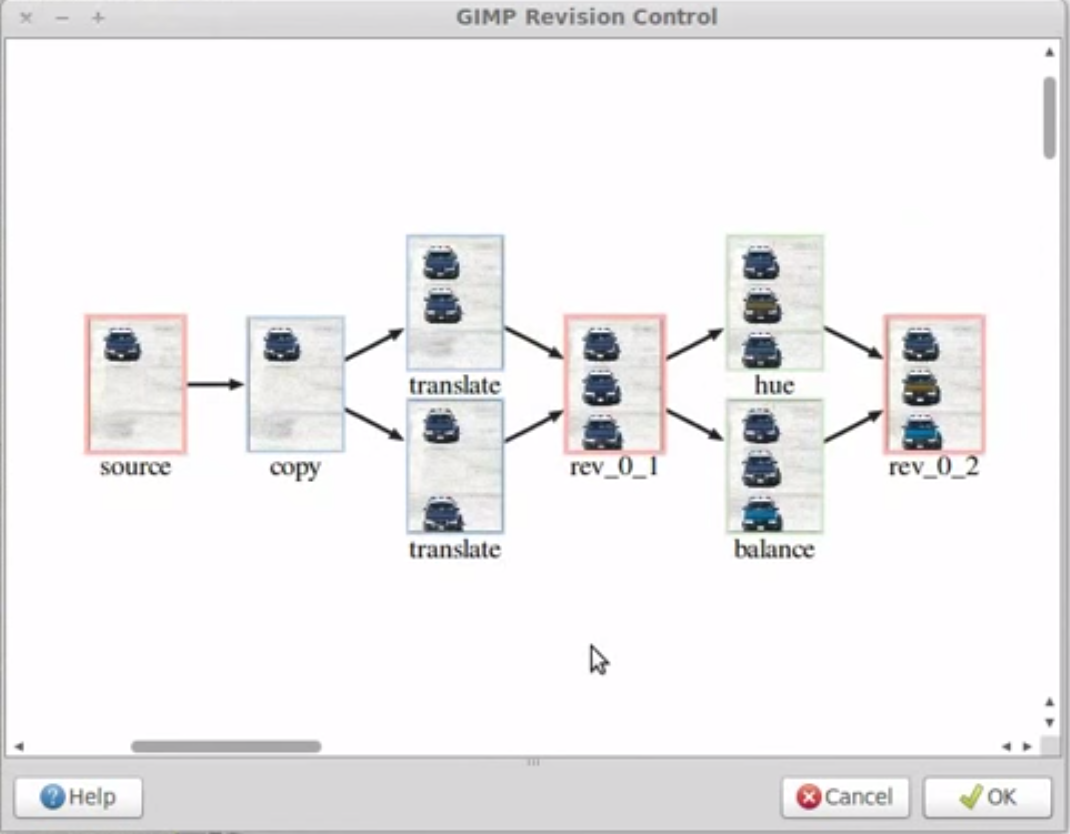
\includegraphics[width=12cm]{related-work/gimp-revision-control}
 \caption{Revision control for GIMP, screenshot taken from introductory video \cite{_nonlinear_????}.}
 \label{fig:gimp-rev-control}
\end{figure}

% source of image:
% how to reference?
% http://www.ht-timchen.com/research/nonlinear-revision-control-for-images/

The system enables users to navigate different versions of a graphics file, compare them (diff) as well as create new branches and merge changes. Furthermore, the user can manually check in new revisions, even though this is generally unnecessary since the system tracks all user actions automatically. Common use cases cited by the researchers are image editing and digital sketching. Especially the latter one often involves trial-and-error experiments that make revision control particularly useful. During usability tests Chen et al. found that participants were happy to integrate revision control features into their workflow. Especially the visual representation of the history was deemed useful. Merging on the other hand, seemed to be more difficult for some users. The researchers conclude that even though the system is easy to use and helpful it might take some time and practice to master it.

\section{Conclusion}
It has become apparent that Git has some conceptual deficiencies that cannot be solved by just creating a new interface. Instead the underlying structure needs to be questioned and features should be redesigned or dismissed. The fact that experienced engineers at renowned software companies were anxious to freely interact with the system is proof that Git has some design flaws. These problems need to be eliminated before Git can be used by a non-technical audience.

On the other hand, fully automated version control does not seem to be the holy grail either. If users are not exposed to version control features at all it decreases the discoverability and might prevent them from forming an accurate mental model of the system. This might handicap their ability to solve problems in case the system does not work as intended. Furthermore, automated version control lacks a fine-grained control of how the work is structured and presented to collaborators (commit messages and history).

The findings of Bicer et al. showed that not every problem a software has can be fixed by adding new features. Sometimes, designers and researchers are better off accepting the boundaries of what software can achieve and focusing on building a lean system that can do everything that is necessary but not more than that. This again highlights the importance of \textit{propriety}, offering only the smallest possible set of features, mentioned by Jackson and Perez De Rosso. Nevertheless, facilitating communication through a version control system is a promising and important feature that should not be ruled out, only because it did not work in one particular setting.

Concluding one could say that Git's conceptual design flaws need to be eliminated and that hidden dependencies should be reduced. This will be a challenging task given that the new system will still be based on Git and Github. Nevertheless, Jackson and Perez de Rosso have shown that enhancements can be made even within the constraints of an existing system.

% State of the Art is described in correct technical and business­-related terms?
% ­Search strategy for literature is explicit and rational?
% ­Quality of the literature analysis: broad and profound (e.g. more articles used)?
% ­Recent and important literature concerning state­ of ­the ­art?
% ­Report gives sufficient arguments to what degree literature can inform the current practice?
% ­Report gives sufficient arguments why findings from current literature can/cannot be applied to innovation project?
% ­Report describes about what clarifications and modifications on concepts from literature need to be taken into account so that findings from current literature become applicable?

\chapter{User \& Task Analysis} \label{chapter:user-research}
Now that the concept of version control and the state of research should be a little clearer, the focus will shift from the abstract and theoretical to more practical matters. This chapter will introduce the reader to the different groups of people involved in creating new language lessons for the Babbel learning platform. In addition to outlining the responsibilities of different user groups, their needs and requirements the most common tasks are analyzed.

Even though the results of this research project should be applicable to a wide range of authoring tools, it is worth noting that, from now on, this thesis will be concerned with the usage of such a system in one particular case: the creation of language lessons by linguistic experts at Babbel. The so called \textit{didactics department} consists of 25 full-time employees and almost 100 freelancers. The department is responsible for creating new language learning content for Babbel's 14 different languages and is divided into teams, based on their language expertise. Right now there are 7 different teams that consist of 2-4 people. Each team is led by a project manager who guides the process of creating new courses and lessons and also manages the collaboration with freelancers.

\section{User Groups}
Below, the different user groups are listed accompanied by a short description of their responsibilities. A more detailed explanation of what these responsibilities entail and which tasks these users perform on a daily basis can be found in the last section.

\subsection{Content Authors}
Content authors conceptualize and create new content. Together with their project managers they decide how a lesson looks like in detail. What is the lesson trying to teach the end-user? What kind of vocabulary is introduced? Which type of exercise is suited best to convey this knowledge? If these decisions are made the editor goes on to "script" a lesson, meaning that a spreadsheet is filled in that defines the exercises, vocabulary items and translations. Please note, that initially there is only one translation (English or German). The job of translating (localizing) a lesson into a new language is usually performed by a separate person since there is rarely a content author who has knowledge of all languages a particular lesson is translated to.

\subsection{Project Managers}
As mentioned above, project managers are the ones who guide the content creation process. They have to set priorities and decide what needs to be worked on. Furthermore, they need to manage freelancers and make sure that they stick to an agreed upon schedule. Project managers are also responsible for the content quality and have the last word before a new course is released.

\subsection{Translators and Proofreaders}
Translators and proofreaders are responsible for localizing lessons into new languages. They get a clearly defined work package and work in unison. First, the translator translates all vocabulary items, exercise titles and descriptions and then hands over her work to the proofreader. The proofreader corrects spelling errors and notes feedback on issues of style, grammar or semantics.

The role of being a translator or proofreader is not permanent, but only true for the duration of a project. Someone who is proofreading during one project could be translating during the next. This is why they are regarded as one user group. A more detailed description of tasks performed by translators and proofreaders can be found in the next chapter in section \ref{sec:task-localization}.

% \subsection{Speakers}
% Speakers may have the most straightforward job. They have to record the individual vocabulary items of a lesson. Of all users they need to collaborate the fewest with other people. Because of that and because it is not clear whether sound recording will be a feature of the new content authoring tool, speakers will be ignored for the rest of the thesis. They are just listed here for the sake of completeness.

\subsection{Quality Assurance Professionals}
Quality assurance is a systematic approach of finding bugs or problems within newly created content. It happens before new content is released. The check is carried out in the frontend as the end-user would use it. The CAT is only used when an error is found and needs to be corrected. A detailed account of what happens during quality assurance is given in section \ref{sec:task-qa}.

\section{Task Analysis} \label{section:task-analysis}
As described in Chapter \ref{chapter:methods}, a hierarchical task analysis was used to analyze the most common tasks performed within the process of authoring new language learning content. Insights were gained through interviews and observations over the course of several weeks. The task analysis in conjunction with the requirements described later on has served as a foundation for the design of the first prototype.

%At first employees at Babbel, working on a particular task, were observed. Based on the notes taken during these sessions a first draft of a task diagram was composed. Later on this diagram was discussed with a member of the didactics team during an informal interview. The interviewee was not necessarily the same person that had been observed. With the feedback from the interviews the diagrams were improved again and finalized. The people that participated in these sessions were all full-time Babbel employees, because getting hold of freelancers is much more difficult, since they live in all parts of the world and not necessarily in Berlin, Germany, where Babbel is based. Nevertheless, some valuable feedback could be gathered from Babbel employees that were freelancers themselves before they started working full-time for Babbel.

%\subsection{User Groups Involved}
%The tasks that are listed in table \ref{table:analyzed-tasks} are performed by different user groups. Often these tasks require a close collaboration between users. In the case of full-time employees this collaboration is typically a little easier, because they work in the same building and can communicate face to face. Freelancers use Google Sheets \cite{_overview_????} for recording feedback and then might discuss it via telephone later on.

%The initial creation of new courses and lessons is done by full-time employees at Babbel. Usually a project manager guides the process and the content editors in the team support him in actually creating the content. In contrast to that the localization of this content is almost exclusively carried out by freelancers. Only the first step of setting up the content for the localization is performed by internal employees at Babbel. The remaining work is done by freelance translators and proofreaders. The following section paints a more detailed picture of how this process actually looks like.
% is this needed here or can it be included into later sections?

\subsection{Tasks} \label{tasks}
It is the responsibility of the didactics department to constantly create new learning content. This work can be divided into three major tasks, which can be seen in Table \ref{table:analyzed-tasks}. Three of these four major tasks were analyzed and then visualized using a diagram that shows the hierarchy and dependencies of different sub-tasks. Task 3 was not analyzed, because it is performed with a different tool and is quite separate as a task from the other ones.

Note that Task 1 and 3 are carried out by employees at Babbel, whereas Task 2 is mostly performed by freelancers.

%The only exception to this is the voice recording workflow, because it is unclear whether the new tool will accommodate this feature in the future. Therefore voice recording was ignored for now. The three following major areas were analyzed.

\begin{table}[h]
\centering
\begin{tabular}{|l|l|}
\hline
\rowcolor[HTML]{EFEFEF}
{\bf Level} & {\bf Task Description}      \\ \hline
0. & Conceptualizing and creating new learning content \\ \hline
1. & Create new lesson           \\
2. & Localize new lesson         \\
%3. & Sound recording for new lesson     \\
3. & Final quality assurance        \\ \hline
\end{tabular}
\caption{Tasks that were analyzed}
\label{table:analyzed-tasks}
\end{table}

\subsubsection{Task 1: Creating a New Lesson}
Figure \ref{fig:build} shows the workflow for creating a new lesson. It should be noted that before a new lesson is entered into the system, as it is described here by the diagram, a long process of conceptualizing (what should we teach the user and in which way?) and scripting already lies behind. What is referred to as scripting is the process of deciding on the right format of the content. For example what exercise types are best suited to convey a particular kind of knowledge about a language. All these decisions are put into a spreadsheet that is called the manuscript, therefore the term scripting. Creating a new course or lesson, as described by the diagram, is thus only a matter of transferring the manuscript into the content authoring tool. Whether this whole workflow can be centralized or combined inside the new tool remains to be seen.

%Please note that compared to the other diagrams the ones in figure \ref{fig:build} and \ref{fig:build-decomp} do not have a grey background highlighting the subtasks that are performed within the content authoring tool. This is because in these diagrams every single sub-task is performed within the tool and therefore the highlighting would have been redundant.

\begin{figure}[h]
 \centering
 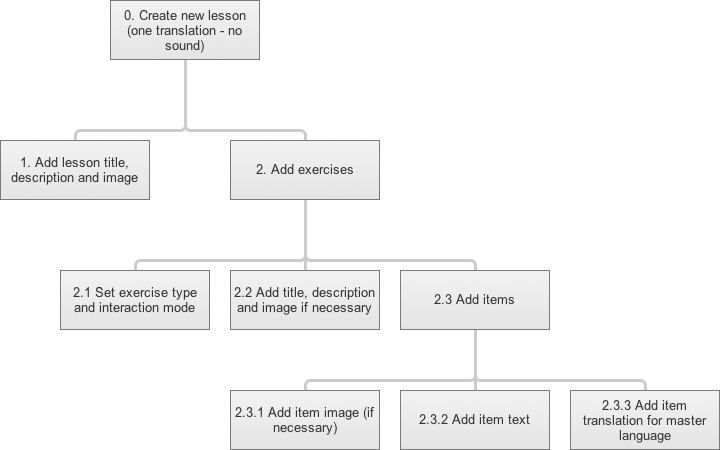
\includegraphics[width=12cm]{images/task-analysis/create_lesson}
 \caption{The tasks involved in creating a new lesson}
 \label{fig:build}
\end{figure}

%\subsubsection{Overview}
%On a high-level scale creating a new lesson or course seems rather simple. Figure \ref{fig:build} visualizes this fact. A new lesson is created within an existing or a new course and then a number of exercises are added. These exercises themselves hold a number of items, representing words or sentences.

%\subsubsection{Creating a New Course/Lesson Decomposed}
%The decomposed tasks now provide a more detailed picture of which subtasks are needed in order to actually create a new lesson. This diagram goes down to the single interactions the user needs to perform in order to reach his or her goal. It is so detailed that it could be used as a how-to-guide for someone who has not used the system before.

\subsubsection{Task 2: Localization of a Lesson} \label{sec:task-localization}
The following diagrams visualize the process of translating existing content into new (display) languages. A display language is the language a user chooses which defines the language of the user interface as well as the translations and explanations he gets while learning a new language. Usually the display language corresponds to the user’s mother tongue, but sometimes learners whose mother tongue is not offered on babbel.com choose English as alternative. Babbel offers 14 different learning languages right now which can be learned by using one of the 8 different display languages. This means that there are more than 100 unique language learning combinations (14*8) that need to be maintained as well as extended when new content is added to a language.

The task of localizing existing content is a joint effort of employees at Babbel and at least two different freelancers. Usually a \ac{PM} at Babbel prepares a content package (several lessons or a whole course) for translation and manages the whole process. Afterwards a freelance translator takes over and translates all the necessary content based on a time plan. When he or she has finished a package the work is handed over to a proofreader who might do some corrections or suggest improvements. Figure \ref{fig:loc-overview} presents a high-level view of the localization process.
% watch out when switching task and user analysis again the project manager appears first in the user analysis

\begin{figure}[h]
 \centering
 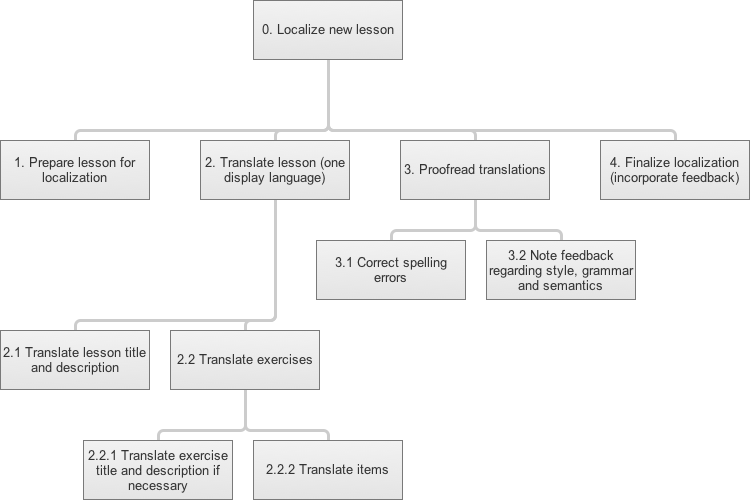
\includegraphics[width=12cm]{images/task-analysis/localize_lesson}
 \caption{Overview of Localization Process}
 \label{fig:loc-overview}
\end{figure}

%\subsubsection{Preparing a Course/Lesson for Localization Decomposed} \label{sec:preparing-loc}
%Before a course or lesson can be translated a few steps are usually necessary to ensure the translator will not encounter any problems during the process. Furthermore it needs to be ensured that end-users are not affected by making the content that is not ready yet invisible to them. This task is usually performed by a project manager.

%\subsubsection{Translation of a Course/Lesson Decomposed}
%Once a course or lesson has been setup for translation the work is handed over to a translator. Figure \ref{fig:loc-trans} shows which subtasks are necessary in order to translate a complete course.

%\subsubsection{Proofreading a Translation Decomposed}
%After the work of the translator is finished the proofreader gets informed. His job is to check the work of the translator for spelling errors or content-related problems. Spelling errors are corrected right away, but instances where the proofreader disagrees with a matter of style or how something is translated are noted in a Google Sheets file and discussed later on. As can be seen in figure \ref{fig:loc-proof} the proofreader only uses the content authoring tool when he or she wants to correct a spelling mistake.

%\subsubsection{Finalizing a Localization Decomposed}
%Finalization means that the translator looks at the comments of the proofreader and implements the suggestions if he or she agrees with them. If not, a discussion between translator and proofreader takes place. They try to settle the issue independently first and only if no agreement can be reached a project manager at Babbel is consulted. When all issues have been resolved the work is handed back to Babbel where the work of the freelancers is evaluated once more by a final quality assurance.

% \subsubsection{Task 3: Image Assignment}
% % still work in progress


% \subsubsection{Task 4: Sound Recording}
% Sound recording is the process of turning the different vocabulary items into speech. Only the learning language is recorded, not the translations. The recordings are done by native speakers who work as freelancers. Whenever new content is ready for recording (usually several lessons or a whole course) the speakers get informed of what exactly needs to be recorded. They can either do this at home, provided they use a high-quality microphone, or come to the Babbel offices and record in a professional studio. Either way, the tool they use, is the same. The recorded sounds end up on the media server and the sound IDs are linked to the respective items. After the speaker has finished his or her work package a full-time employee checks whether the recordings meet the quality standards and if not some sounds need to be re-recorded.

% \begin{figure}[h!]
%  \centering
%  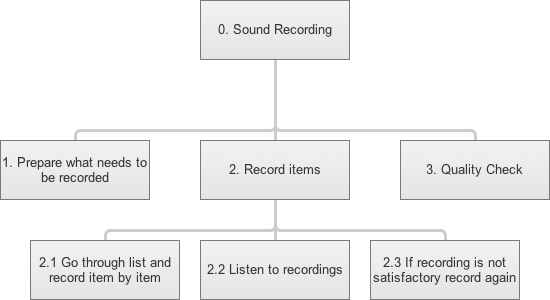
\includegraphics[width=9cm]{images/task-analysis/sound_recording}
%  \caption{Sound Recording Process}
%  \label{fig:sound-recording}
% \end{figure}

\subsubsection{Task 3: Quality Assurance} \label{sec:task-qa}
The final quality assurance happens right before new learning content is published. A Babbel employee clicks through the content in the frontend as a normal Babbel user would. This happens to check whether the content works as expected and the application does not break down at some point because a bug has been introduced. It is also the last chance of spotting spelling or grammar mistakes or checking whether the content complies with different conventions and has a consistent style.

\begin{figure}[h]
 \centering
 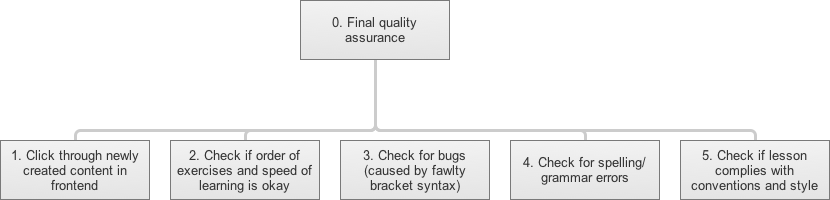
\includegraphics[width=\textwidth]{images/task-analysis/quality_assurance}
 \caption{Quality Assurance Process}
 \label{fig:qa-process}
\end{figure}

\subsection{Conclusion}
The analysis made a few things obvious. First of all, collaborating and communicating with colleagues is a reoccurring theme throughout most tasks. Not only the content creation process is divided between different user groups, but also some tasks themselves. For example, when a lesson is localized, there are at least three different individuals working together, who also need to communicate in some way. Right now, email and Google Sheets are used extensively for that, but it is conceivable that at least some of this communication could be facilitated by the new version control system. This could possibly speed up the whole process and streamline collaboration.

%The preparation of localizations (Figure \ref{fig:loc-overview}) is a good example of a step that could almost completely be avoided with a better interface design. Right now everything needs to be prepared and set up initially to make sure that translators only work on the content they are supposed to work on. In future, when a version control system is in place, it is imaginable to skip this process, because work will not be performed on live data anymore and reversibility of changes will be simpler.

In general, version control features could potentially ease collaboration and allow full-time employees to give freelancers more freedom in their work, because the risk of breaking live content will be lower. Furthermore, a feature similar to Github's \textit{pull request} could help to formalize the quality checks that happen throughout the process and provide a platform for communication between freelancers and full-time employees.

The next section introduces a list of formalized requirements that have been partially derived from the analysis of user groups and their daily tasks.

\section{Requirements}
As described in Chapter \ref{chapter:methods} this analysis was based on observations and interviews with members of the Didactics Department at Babbel. First, functional requirements are listed, which describe requirements based on a user's goal. In Section \ref{sec:quality-requirements} the quality requirements of the whole system are explained.
Please be aware that the following requirements are only concerned with the version control aspects of the content authoring tool. The list of requirements for the whole tool would contain much more.

%The requirements are related to the new content authoring tool and the version control capabilities in particular. They are purely functional and will help to ensure that the final satisfies the various user needs. The requirements were gathered through observations and interviews that were also carried out for the task analysis described earlier.

% the requirements are based on the task analysis

\subsection{Functional Requirements}
The functional requirements are grouped based on the different user groups. Please note that these user groups are only approximations of the user's responsibilities and in reality are not as clear cut as it might seem here. For example, project managers share many requirements with content authors and the role of translators and proofreaders could be regarded as interchangeable as well.

The requirements are phrased as user stories, which emphasise the user's perspective and the ultimate goal they are trying to achieve by using the software.

%\subsubsection{Requirements of Project Managers}

\begin{table}[h!]
\centering
\begin{tabular}{|l|p{12cm}|}
\hline
\rowcolor[HTML]{EFEFEF}
\textbf{\#} & \textbf{Requirement} \\ \hline
PM-1 & As a project manager I want to make sure that translators only work on the content they are supposed to work on so that no unnecessary work is done by them. \\ \hline
PM-2 & As a project manager I want to have an overview that tells me whether content is broken or something needs attention. \\ \hline
PM-3 & As a project manager I want to know which recent changes have been made to the language package I am responsible for. \\ \hline
PM-4 & As a project manager I want to control when new content is published. \\ \hline
PM-5 & As a project manager I want to know which content is published and which content is currently being worked on. \\ \hline
PM-6 & As a project manager I want to know when translators or content authors have finished their work so that I can review it. \\ \hline
\end{tabular}
\caption{Project manager requirements}
\label{my-label}
\end{table}
% so that is often missing from these requirements

%\subsubsection{Requirements of Content Authors}

\begin{table}[h!]
\centering
\begin{tabular}{|l|p{12cm}|}
\hline
\rowcolor[HTML]{EFEFEF}
\textbf{\#} & \textbf{Requirement} \\ \hline
CA-1 & As a content author I want to be able to edit content at any given moment so that I can be most efficient during my working hours. \\ \hline
CA-2 & As a content author I want to be sure that I cannot break content while editing so that I can focus on what to edit and not how to edit. \\ \hline
CA-3 & As a content author I want to collaborate with my colleagues on new content that I create. \\ \hline
CA-4 & As a content author I want an overview of what I have changed during a session so that I can make sure that all the changes were intentional. \\ \hline
CA-5 & As a content author I want to signal my project manager that I am done with my work so that the PM can review it. \\ \hline
CA-6 & As a content author I want to edit content without fear of accidentally changing the live content so that I can experiment with some changes. \\ \hline
\end{tabular}
\caption{Requirements of Content Authors}
\label{req-content-authors}
\end{table}


%\subsubsection{Requirements of Translators}

\begin{table}[h!]
\centering
\begin{tabular}{|l|p{12cm}|}
\hline
\rowcolor[HTML]{EFEFEF}
\textbf{\#} & \textbf{Requirement} \\ \hline
TL-1 & As a translator I want certainty that I am only translating content that is ready for translation so that I do not translate content that is not ready yet. \\ \hline
TL-2 & As a translator I want to exactly know what I am supposed to translate. \\ \hline
TL-3 & As a translator I want to inform the proofreader when my translations are ready for proofreading. \\ \hline
TL-4 & As a translator I want to get an overview of what changes a proofreader has made to my content. \\ \hline
TL-5 & As a translator I only want to see the information that is important for my job so that I am not distracted and can do my job efficiently. \\ \hline
TL-6 & As a translator I want to be guided through the complex parts of the interface or given a tutorial so that I can focus on my job instead of learning a complex interface. \\ \hline
\end{tabular}
\caption{Requirements of translators}
\label{table:req-translators}
\end{table}

%\subsubsection{Requirements of Proofreaders}

\begin{table}[h!]
\centering
\begin{tabular}{|l|p{12cm}|}
\hline
\rowcolor[HTML]{EFEFEF}
\textbf{\#} & \textbf{Requirement} \\ \hline
PR-1 & As a proofreader I want to know exactly what I am supposed to proofread. \\ \hline
PR-2 & As a proofreader I want to be able to provide feedback to the translator or comment on particular translations. \\ \hline
PR-3 & As a proofreader I want to inform the translator when I have finished my work so that he or she can review what I did as soon as possible. \\ \hline
PR-4 & As a proofreader I want an interface with a minimal set of features so that I can focus on the process of proofreading. \\ \hline
PR-5 & As a proofreader I want to check how the content will look like to the end-user so that I can also check whether the text length is appropriate. \\ \hline
PR-6 & As a proofreader I want to be guided through the complex parts of the interface or given a tutorial so that I can focus on my job. \\ \hline
\end{tabular}
\caption{Requirements of proofreaders}
\label{req-proofreaders}
\end{table}

%\subsubsection{Requirements of QA Professionals}

\begin{table}[h!]
\centering
\begin{tabular}{|l|p{12cm}|}
\hline
\rowcolor[HTML]{EFEFEF}
\textbf{\#} & \textbf{Requirement} \\ \hline
QA-1 & As a QA professional I want to compare 2 different content releases so that I can see what has changed and identify possible problems. \\ \hline
QA-2 & As a QA professional I want to see what has changed within a certain content package so that I know which parts of the content I need to review. \\ \hline
\end{tabular}
\caption{Requirements of QA Professionals}
\label{req-qa-professionals}
\end{table}

%\section{Conclusion}
% it is a diverse set of requirements
% different user groups use tool in completely different ways
% diff view is important for QA proffessionals
% a lot of requirements are about communication and collaboration

%The user requirements are broken down into four parts for the four different user groups. Table \ref{table:requirements-pm} shows the requirements for project managers, that are exclusive to them. Project managers are, speaking in programming-terms, a subclass of content editors. They both share the same responsibilities, but project managers have a few additional ones, such as guiding the content creation process and managing freelancers. The requirements of content editors can be seen in table \ref{table:requirements-editors}. The third and fourth user groups are translators and proofreaders respectively (Table \ref{table:requirements-translators} \& Table \ref{table:requirements-proofreaders}), which together perform the major part in the localization process.

\clearpage

\subsection{Quality Requirements} \label{sec:quality-requirements}
The functional requirements above mostly answered the question \emph{what} specifically users want to do with the tool. The quality requirements instead look at the \emph{how}. The product quality model defined by the ISO/IEC standard 25010 \cite{_iso/iec_2011} names usability as one of eight product characteristics that contribute to the overall quality. Usability is further divided into a set of 6 sub-characteristics: appropriateness recognizability, learnability, operability, user error protection, user interface aesthetics and accessibility. Since the constraints of this project did not allow focusing on all of these aspects, learnability and user error protection were chosen as the most important. Table \ref{table:quality-requirements} shows a list of quality requirements.

\begin{table}[h!]
\centering
\begin{tabular}{|l|p{12cm}|}
\hline
\rowcolor[HTML]{EFEFEF}
\textbf{\#} & \textbf{Requirement} \\ \hline
1 & Users shall be able to start using the system without prior training. \\ \hline
2 & The system shall be pro-active in offering help and advice. \\ \hline
3 & Users shall be prevented from making errors wherever possible. \\ \hline
4 & Errors shall not lead to permanent consequences, reverting should be easy. \\ \hline
\end{tabular}
\caption{Quality requirements}
\label{table:quality-requirements}
\end{table}

% this is strongly connected to the research questions, maybe mention/link them?




% how about adding some quality requirements? usability, learnability etc.


\chapter{First Design Iteration} \label{chapter:design-first-iteration}
% LINK
The analysis presented in the previous chapter has shown that the content authoring process at Babbel is a highly collaborative process involving a lot of tasks. In order to simplify the collaboration and potentially speed up the content creation, the integration of version control features has been suggested earlier.

% FOCUS / AIM - Why is this important?
This chapter describes an early prototype, which exposed several version control features, which were deemed potentially useful for the content authoring process. Since the research presented throughout this thesis was mainly concerned with the applicability of version control to the content creation process, the prototype is an important first step towards answering this research question.

% OVERVIEW
The chapter starts by highlighting the main differences between the integrated version control features and those of a more traditional VCS. Afterwards, the most important views comprising the prototype are shown and shortly explained. Figure \ref{fig:main-views-diagram} might help to visualize the relations between them: The main editing view as well as the diff comparison are very central, whereas the remaining features are more or less equally important. Please note that the diff is not an independent view of itself but is embedded in several other views, such as the history, the saving page and the merge request details.

\begin{figure}[h!]
 \centering
 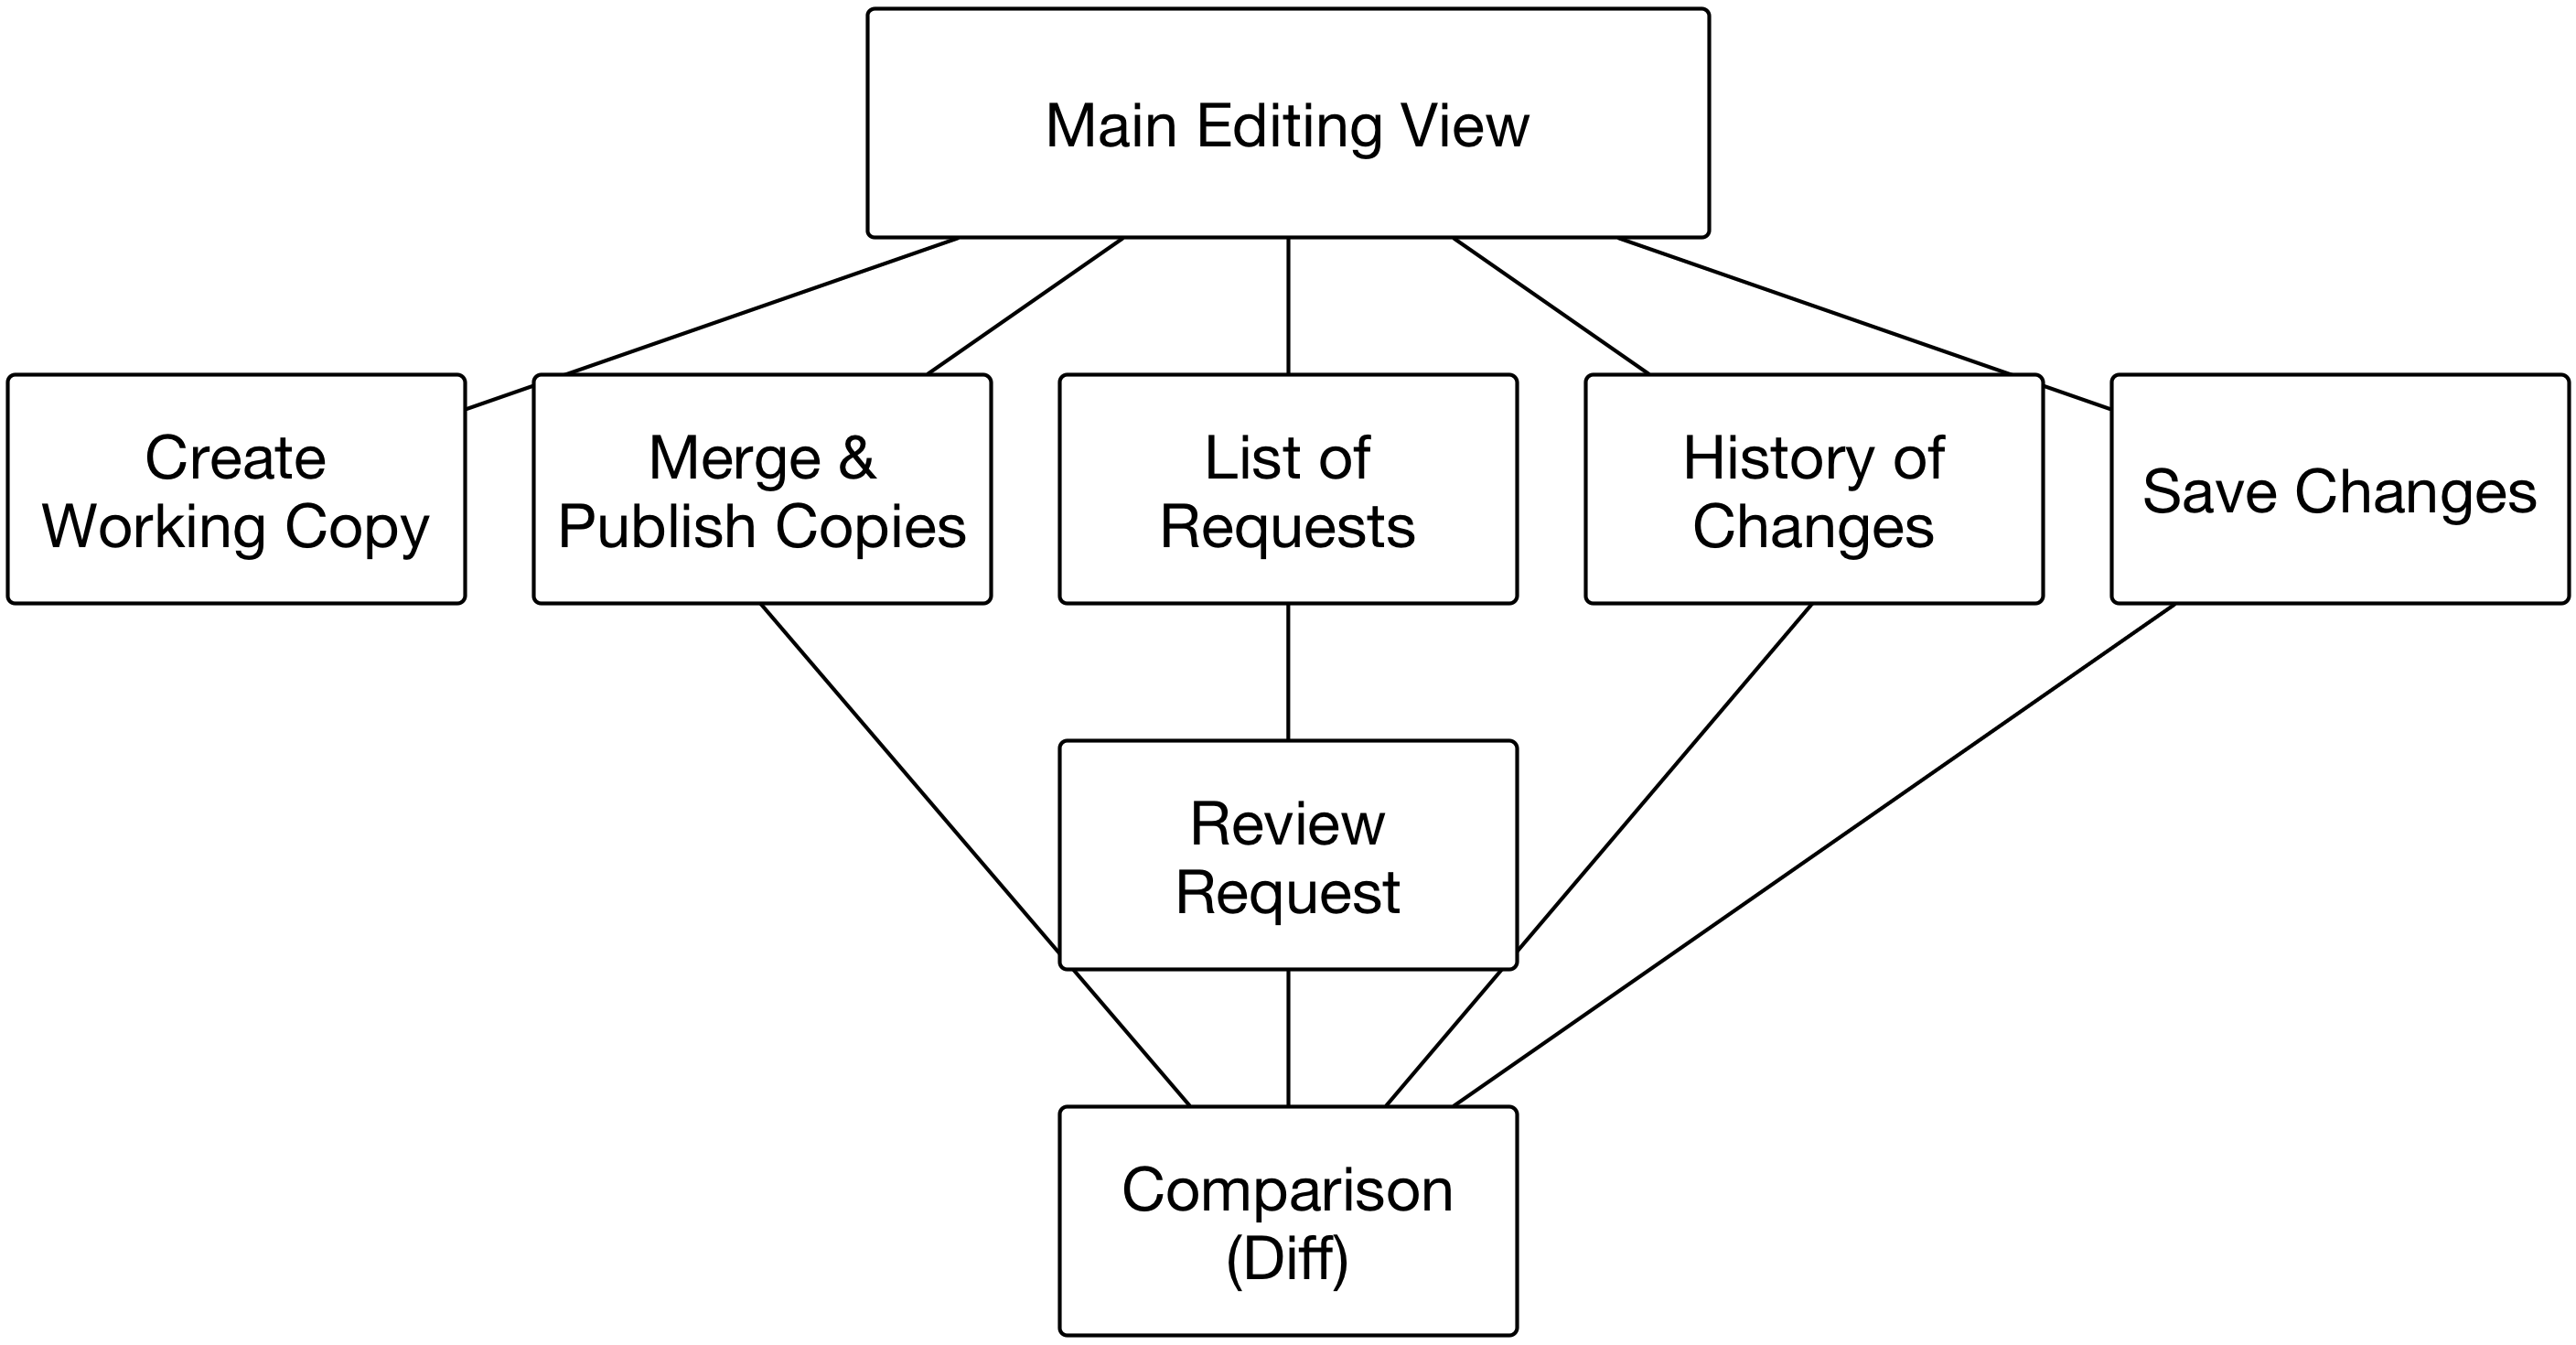
\includegraphics[width=10cm]{second-iteration/main-views-diagram}
 \caption{Overview of main sections of the application}
 \label{fig:main-views-diagram}
\end{figure}

\section{Comparison to Traditional VCSs} \label{sec:git-feature-comparison}
As compared to most other version control systems the interface only offers a minimal set of features. Some of them have been vastly simplified or adapted to the domain of language content authoring. A few features, such as the pull request and the history, are very close to their "originals".

\begin{itemize}
  \item There is no differentiation between \textit{local} and \textit{remote} repositories anymore. Church et al.'s \cite{church_case_2014} work has shown that hidden dependencies between these two repositories often complicate matters for the user. Therefore, it was decided to have only one repository that is constantly up to date. This should, in theory, also simplify collaboration and avoid conflicts.
  \item Specifically \emph{tracking} files is not necessary. Every course or lesson that is created using the tool will be under version control.
  \item There is no \emph{staging} area anymore. As mentioned in Chapter \ref{chapter:related-work} this feature is sometimes problematic and often inconvenient, because every change has to be staged before it can be saved (committed).
  \item The \emph{diff(erence)} view is presented by default before the user saves his or her changes. This ensures that the user knows what will be saved and provides an additional review mechanism. When using the Git CLI, diff is a separate command that needs to be executed when the user wants to look at the things that have changed.
  \item The diff view is enriched by a domain-specific design. It does not only display bare data as represented in the data format, but shows images, allows listening to sounds and visualizes boolean values, so that reviewing changes becomes simpler and is easier for users with a non-technical background.
  \item A \emph{pull request} feature (as on Github) was added. Because Git offers no formalized way of reviewing code before it is merged, this feature enforces best practices. Furthermore, the user analysis has shown that reviewing new content, which was produced by freelancers, is very important.
  %\item Merging is always routed through a pull request, which allows users to review what has changed before merging branches. This reduced the abstraction as compared to merging only based on branch names.
  \item Visualizations were added in order to help users understand some of the more abstract concepts, such as branches. This was inspired by Bitbucket, which is using different visualizations to explain certain features.
\end{itemize}

\section{Prototype}
The overall interface was strongly influenced by existing code hosting platforms, such as Github\footnote{https://github.com/about}, Gitlab\footnote{https://about.gitlab.com/} and Bitbucket\footnote{https://bitbucket.org/} as well as several Git GUIs\footnote{http://git-scm.com/downloads/guis}. The system can be regarded as a crossbreed between version control and content authoring tool. Below, the main views of the prototype are shown.

\subsection{Navigation}
The upper-most navigation bar (Figure \ref{fig:navigation-top}) offers a quick access to the most important version control features as well as the language package and the current branch. Next to the branches dropdown a little plus-icon signifies how a new branch can be created. Furthermore, some buttons provide additional information, such as indicating whether changes can be saved or open pull requests exist.

\begin{figure}[h!]
 \centering
 \fbox{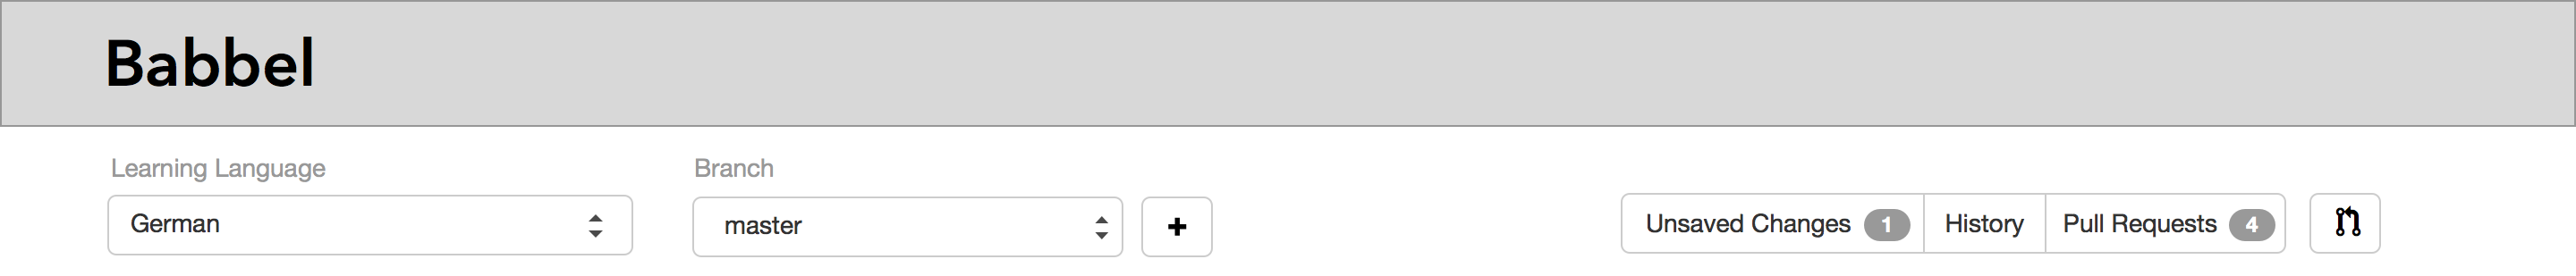
\includegraphics[width=\textwidth]{first-prototype/navigation-top}}
 \caption{The top-bar navigation exposing version control features}
 \label{fig:navigation-top}
\end{figure}

\subsection{Branches}
Branching is a fundamental concept of most version control systems and allows working in an isolated state. A lot of time went into the consideration of whether to include this feature or not. Finally, it was decided, to make this feature visible to users, which has the advantage of them being able to share branches with colleagues or point to a particular state of content that is still being created.

\begin{figure}[h!]
 \centering
 \fbox{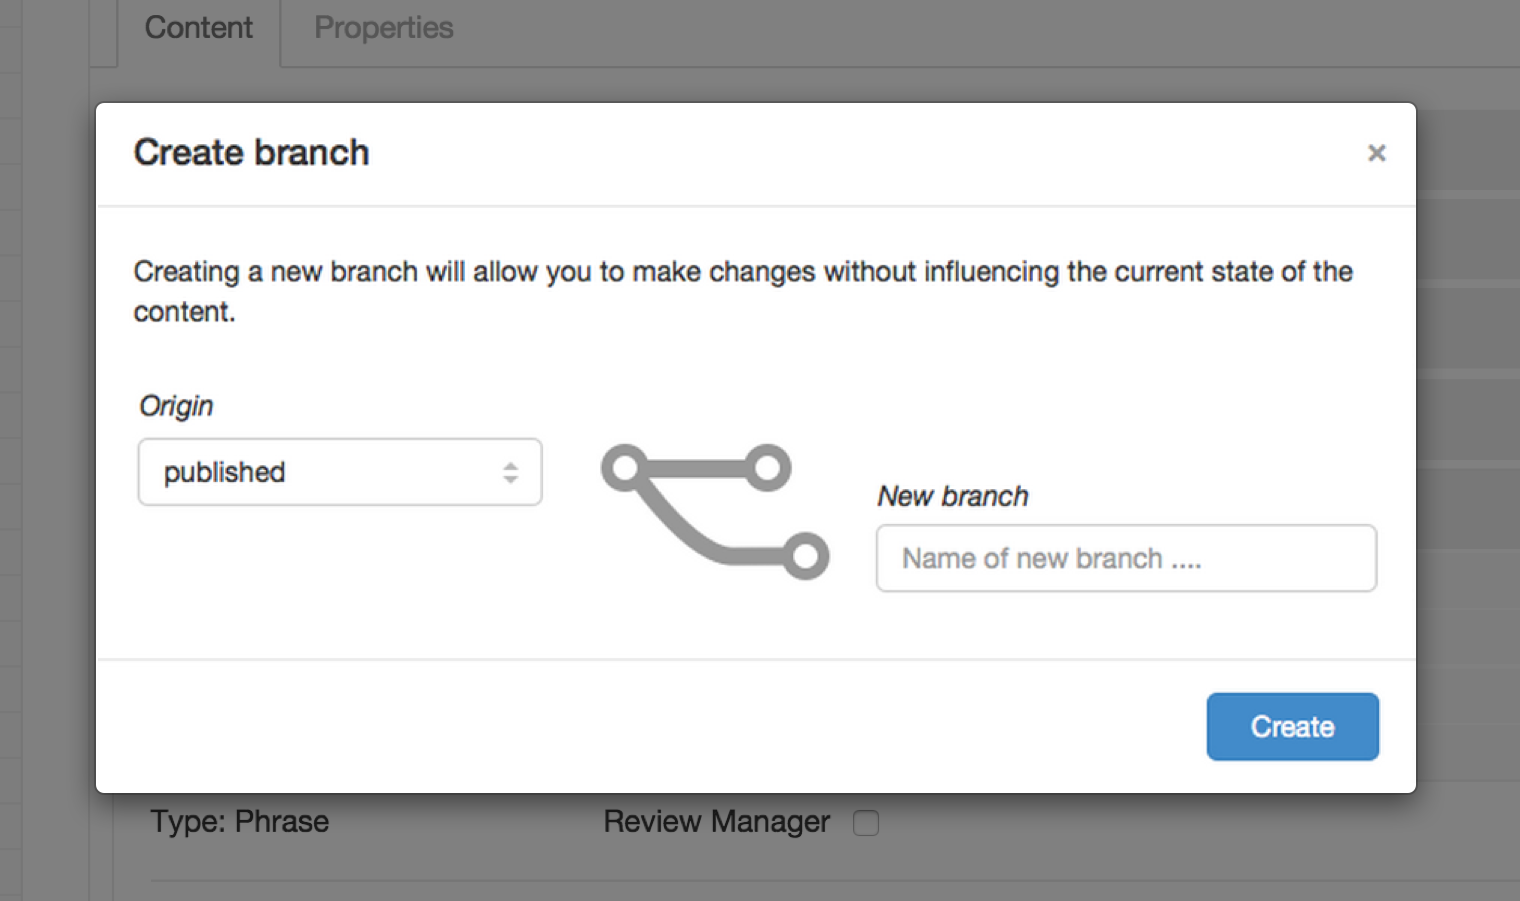
\includegraphics[width=10cm]{first-prototype/create-branch-modal}}
 \caption{The modal allowing users to create new branches}
 \label{fig:create-branch}
\end{figure}

\subsection{Saving Process and Diff View}
As mentioned before, when a user has edited some content, which shall be saved, a difference view is presented. This allows the user to review her changes before committing to a change. As is common with most version control systems, a commit message needs to be entered before saving. This allows collaborators to comprehend why a particular piece of content was edited.

\begin{figure}[h!]
 \centering
 \fbox{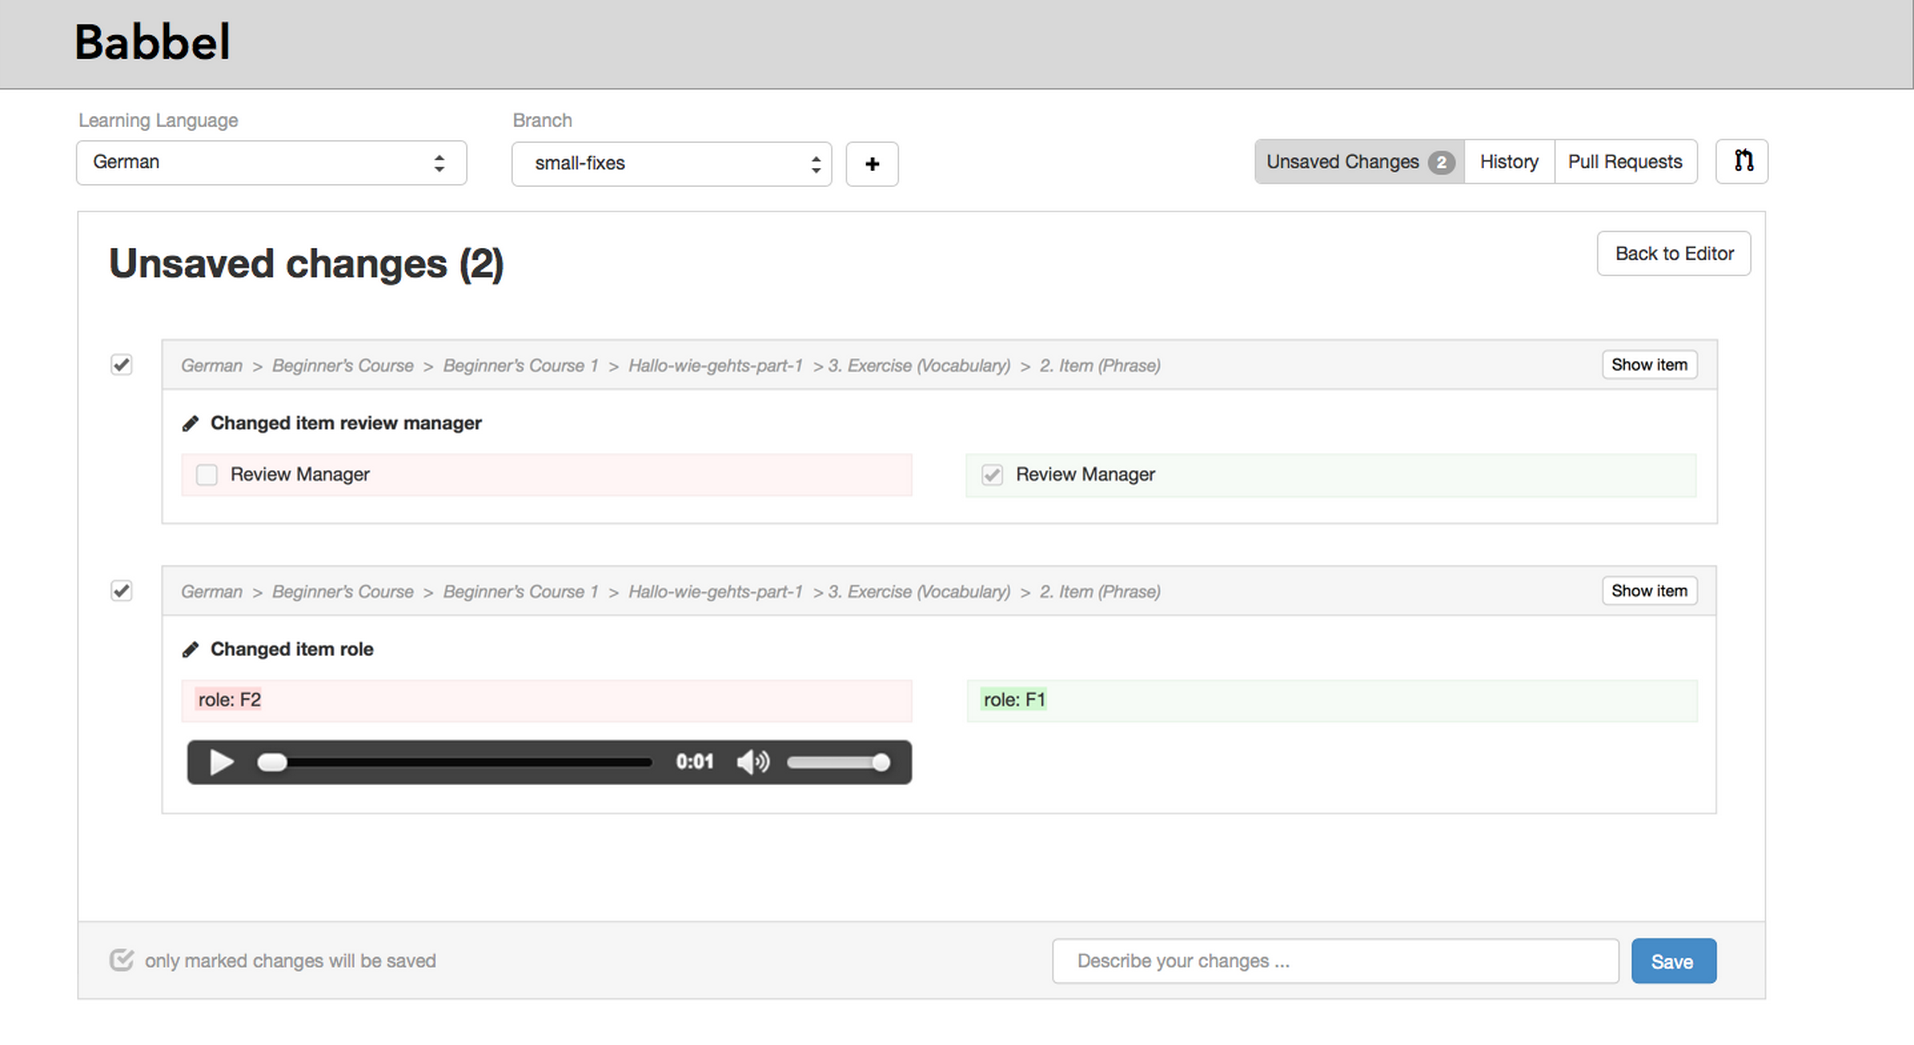
\includegraphics[width=\textwidth]{first-prototype/unsaved-changes}}
 \caption{The difference view highlighting changes the user did recently}
 \label{fig:unsaved-changes}
\end{figure}

\subsection{Content Editing}
The content in the editing view can be navigated by expanding a tree structure (Figure \ref{fig:prot-initial-editor-view}, left-hand side), which also reflects the inherent composition of the content. Furthermore, when a lesson is selected, its exercises are listed and the content can be exposed through so-called accordions. Each exercise consists of several items which themselves consist of text, images and sounds.

\begin{figure}[h!]
 \centering
 \fbox{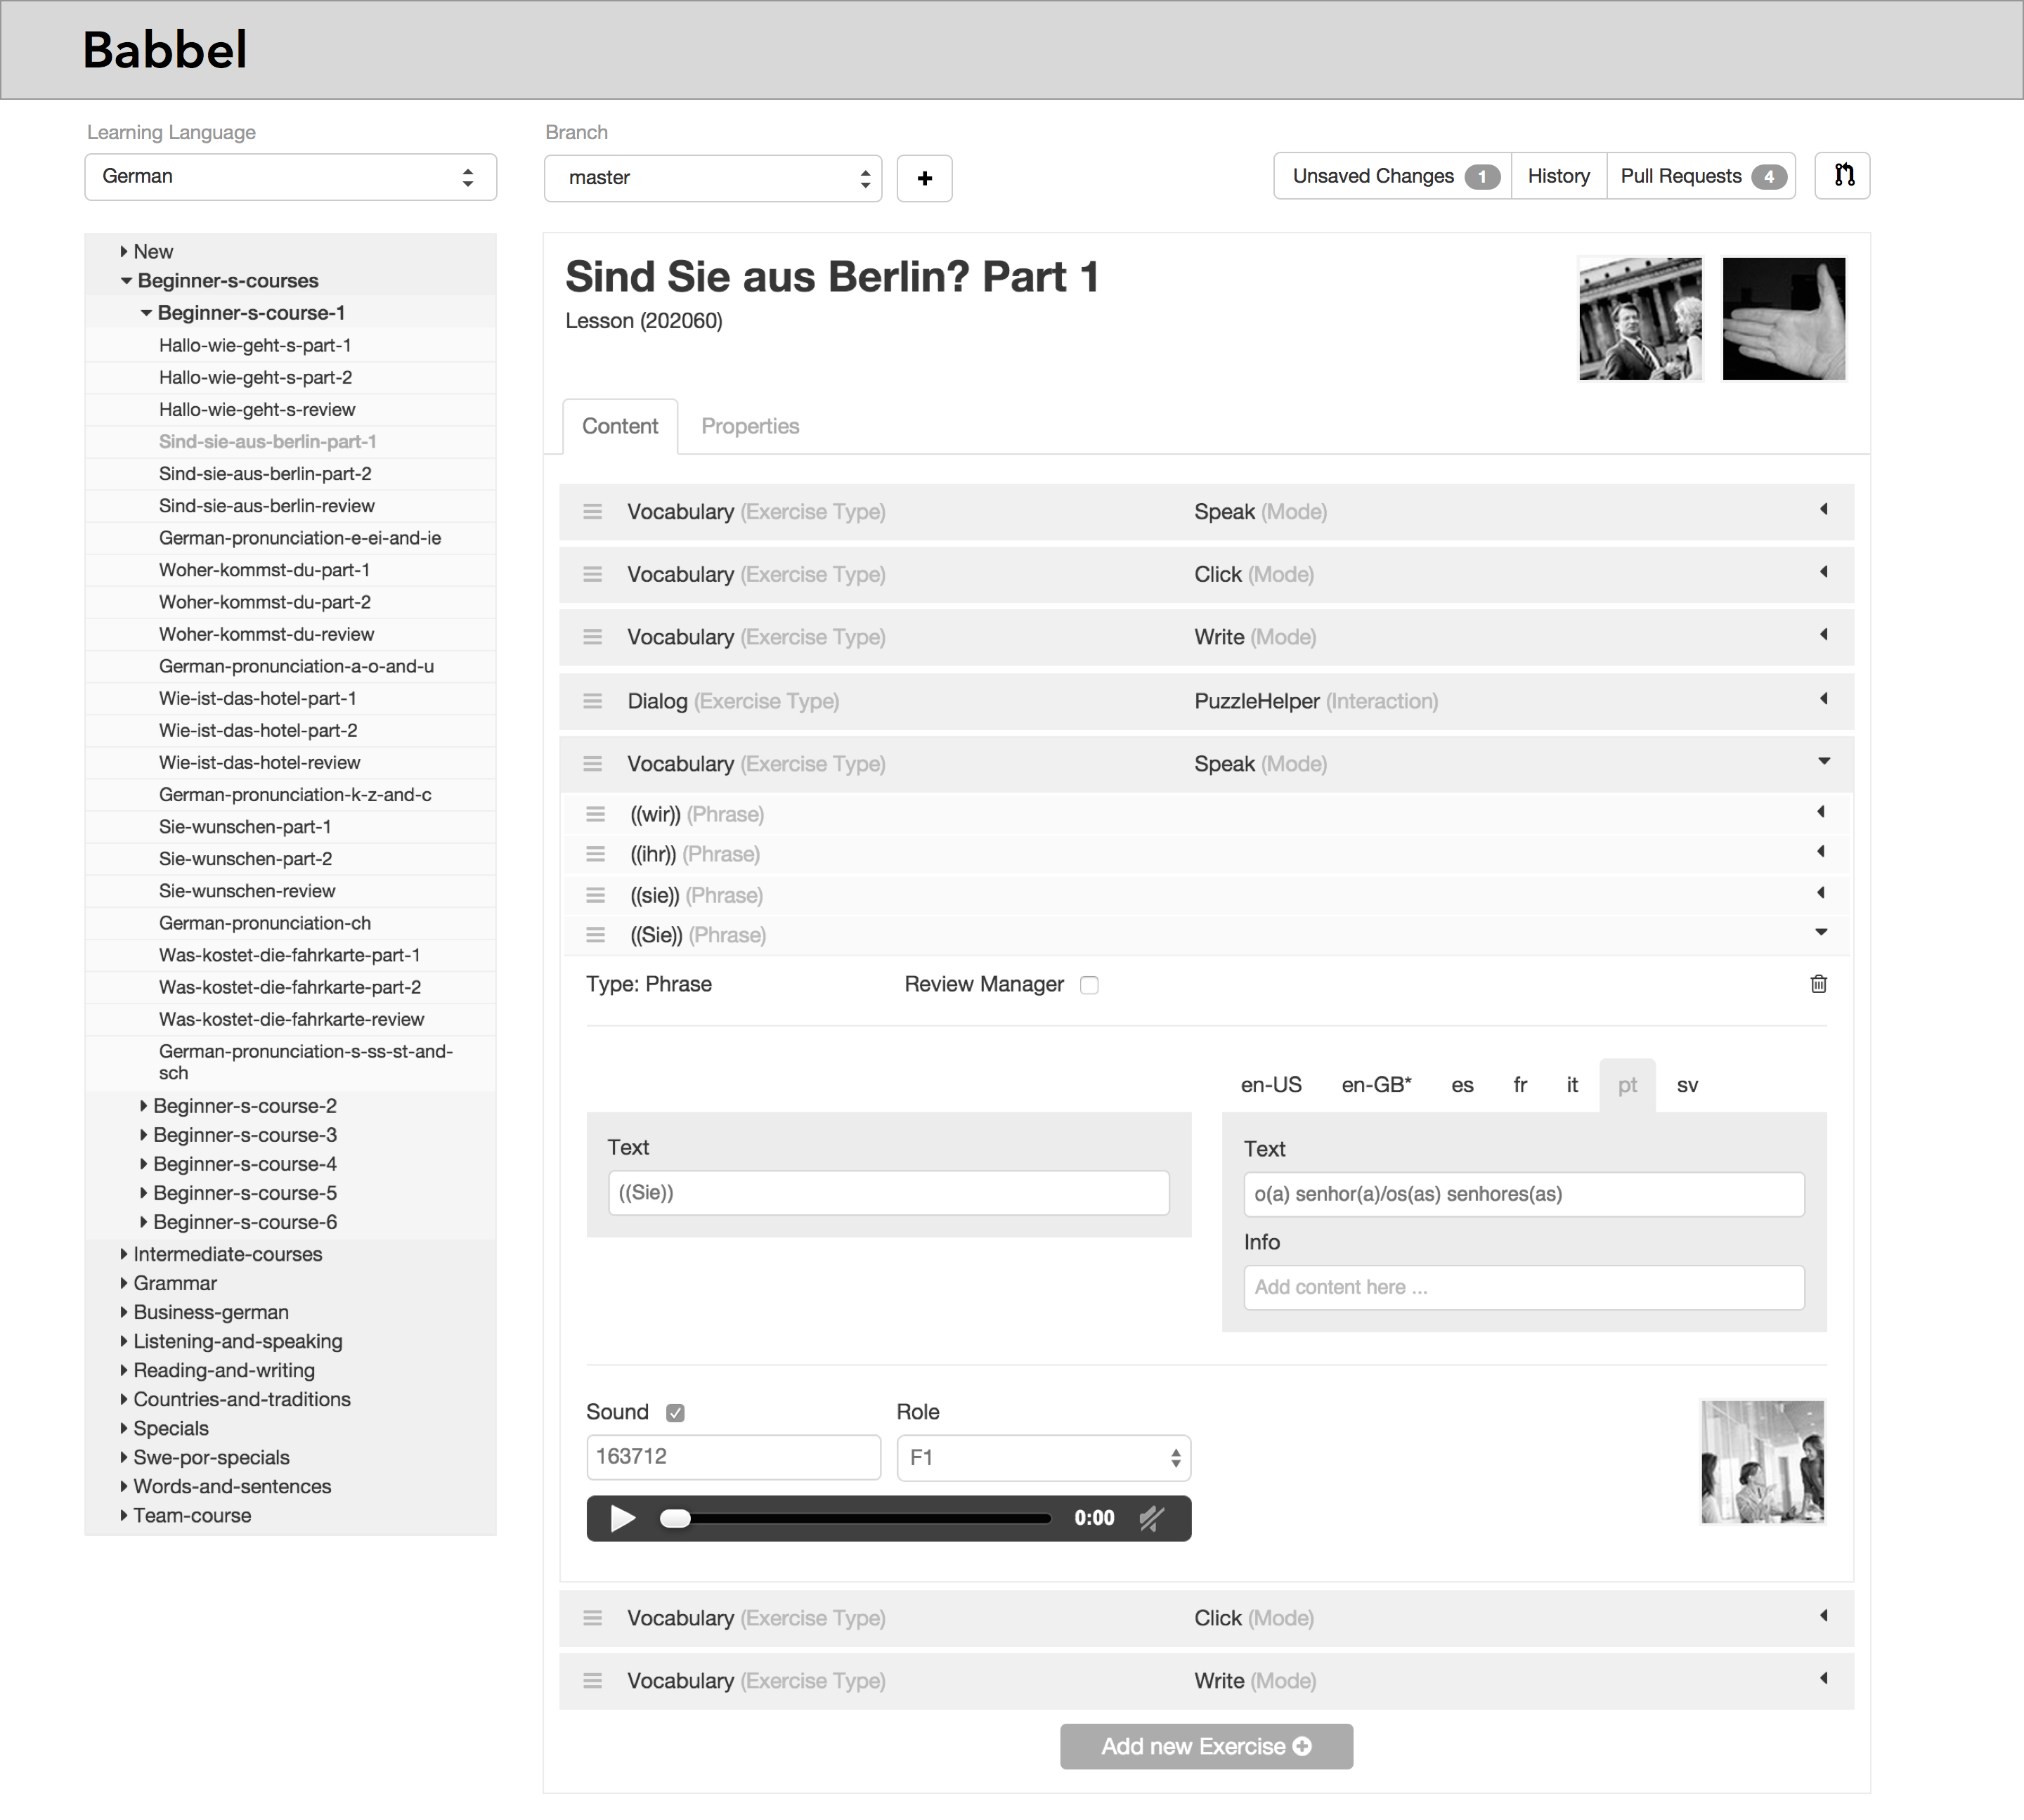
\includegraphics[width=\textwidth]{first-prototype/main-editing-view}}
 \caption{The main editing view with an opened lesson}
 \label{fig:prot-initial-editor-view}
\end{figure}

\subsection{Pull Request}
Pull requests are a formalized way of requesting a "merge" of two branches. A typical version control flow consists of creating a new branch, editing some content, saving it and finally creating a pull request (Figure \ref{fig:open-new-pr}). A pull request allows collaborators to review changes before merging them with the main branch and thus ensures the quality of the content.

\begin{figure}[h!]
 \centering
 \fbox{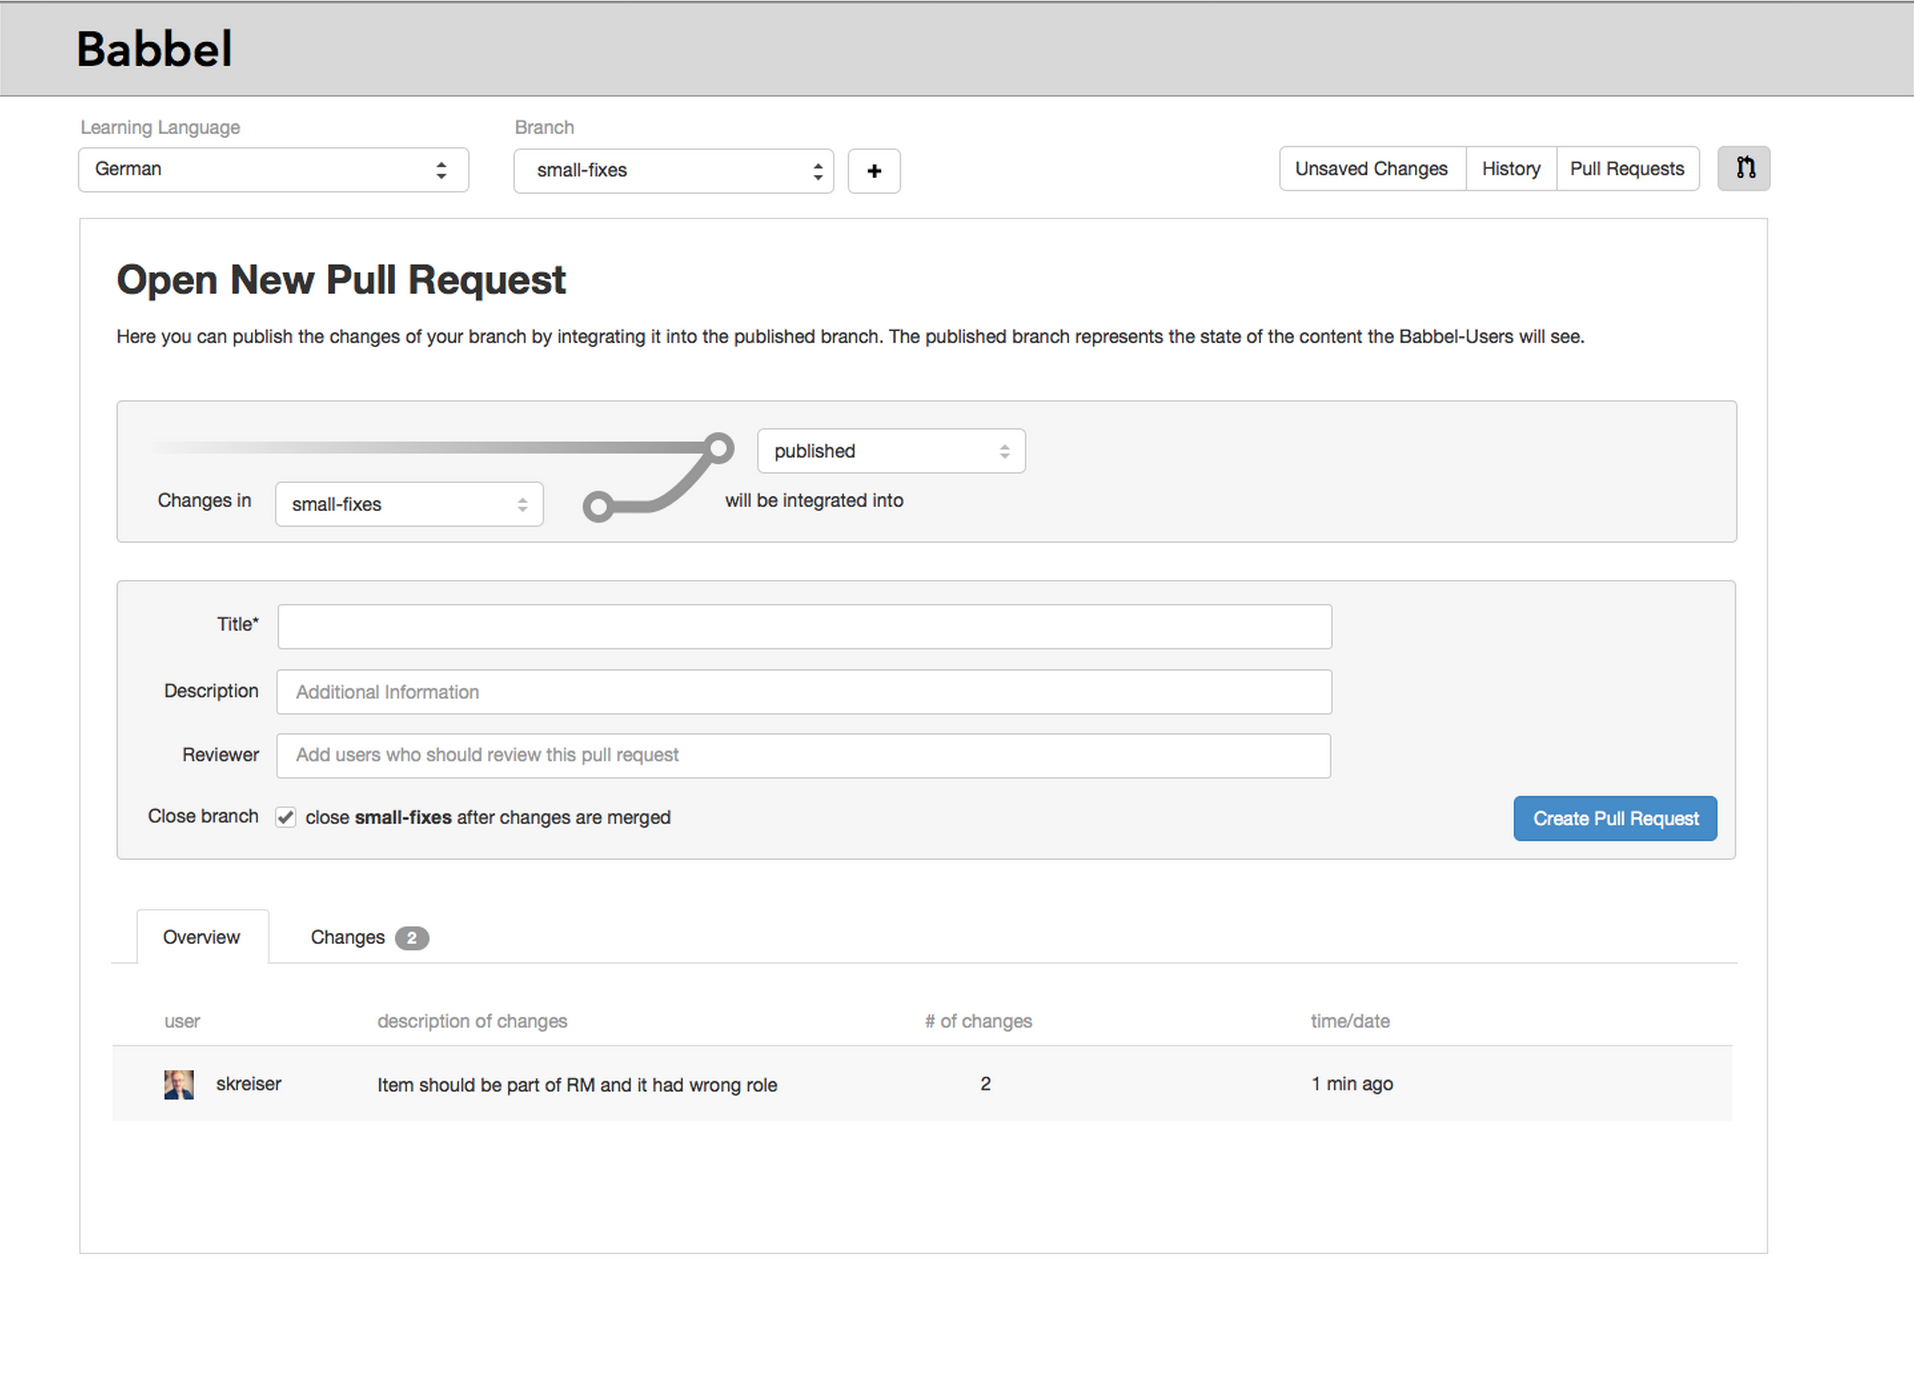
\includegraphics[width=\textwidth]{first-prototype/open-new-pr}}
 \caption{Form allowing the creation of new pull requests}
 \label{fig:open-new-pr}
\end{figure}

% \begin{figure}[h!]
%  \centering
%  \fbox{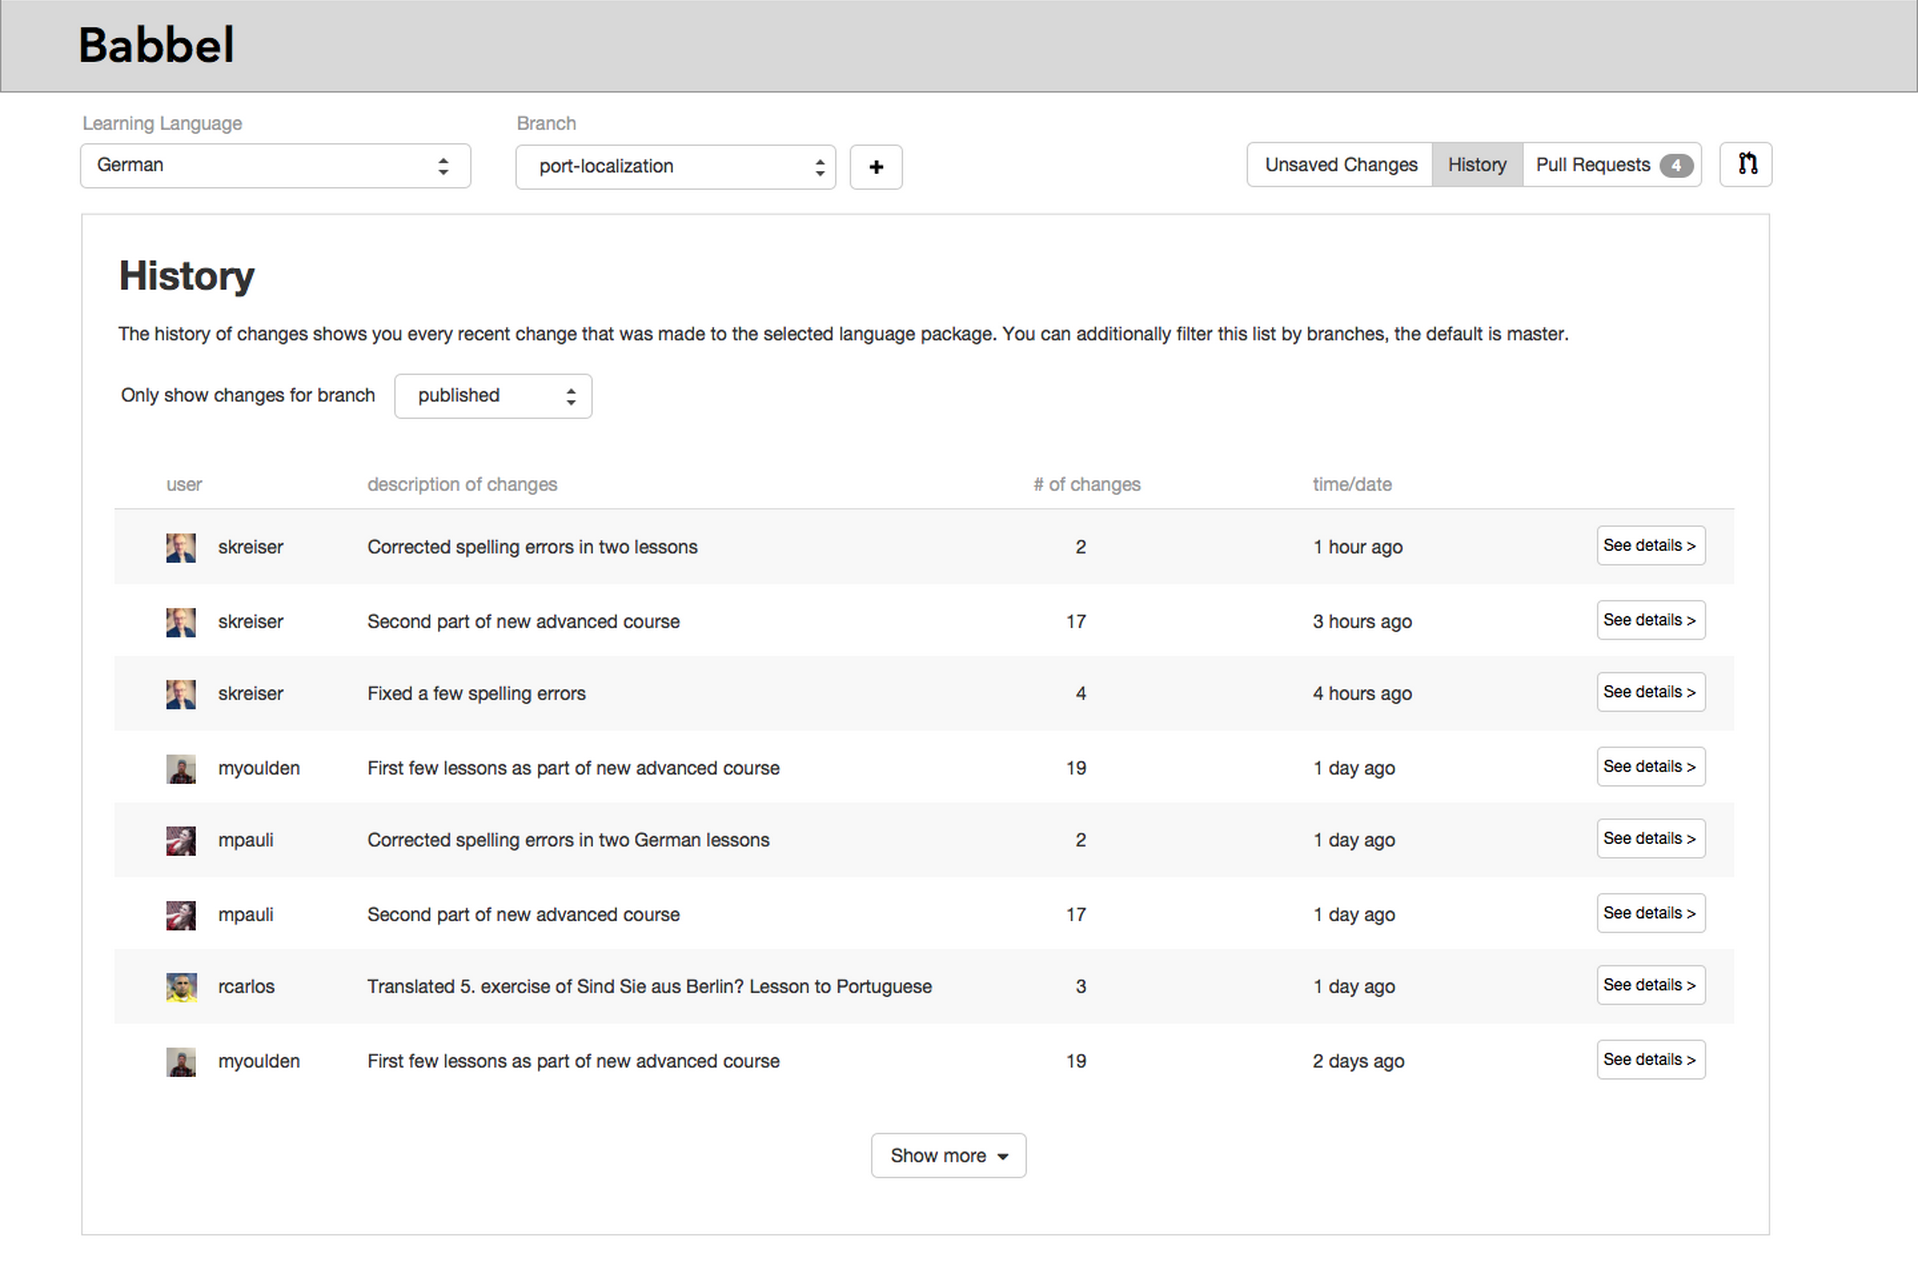
\includegraphics[width=\textwidth]{first-prototype/history}}
%  \caption{The history is a list of recent changes in a particular language package}
%  \label{fig:history}
% \end{figure}


% \begin{figure}[h!]
%  \centering
%  \fbox{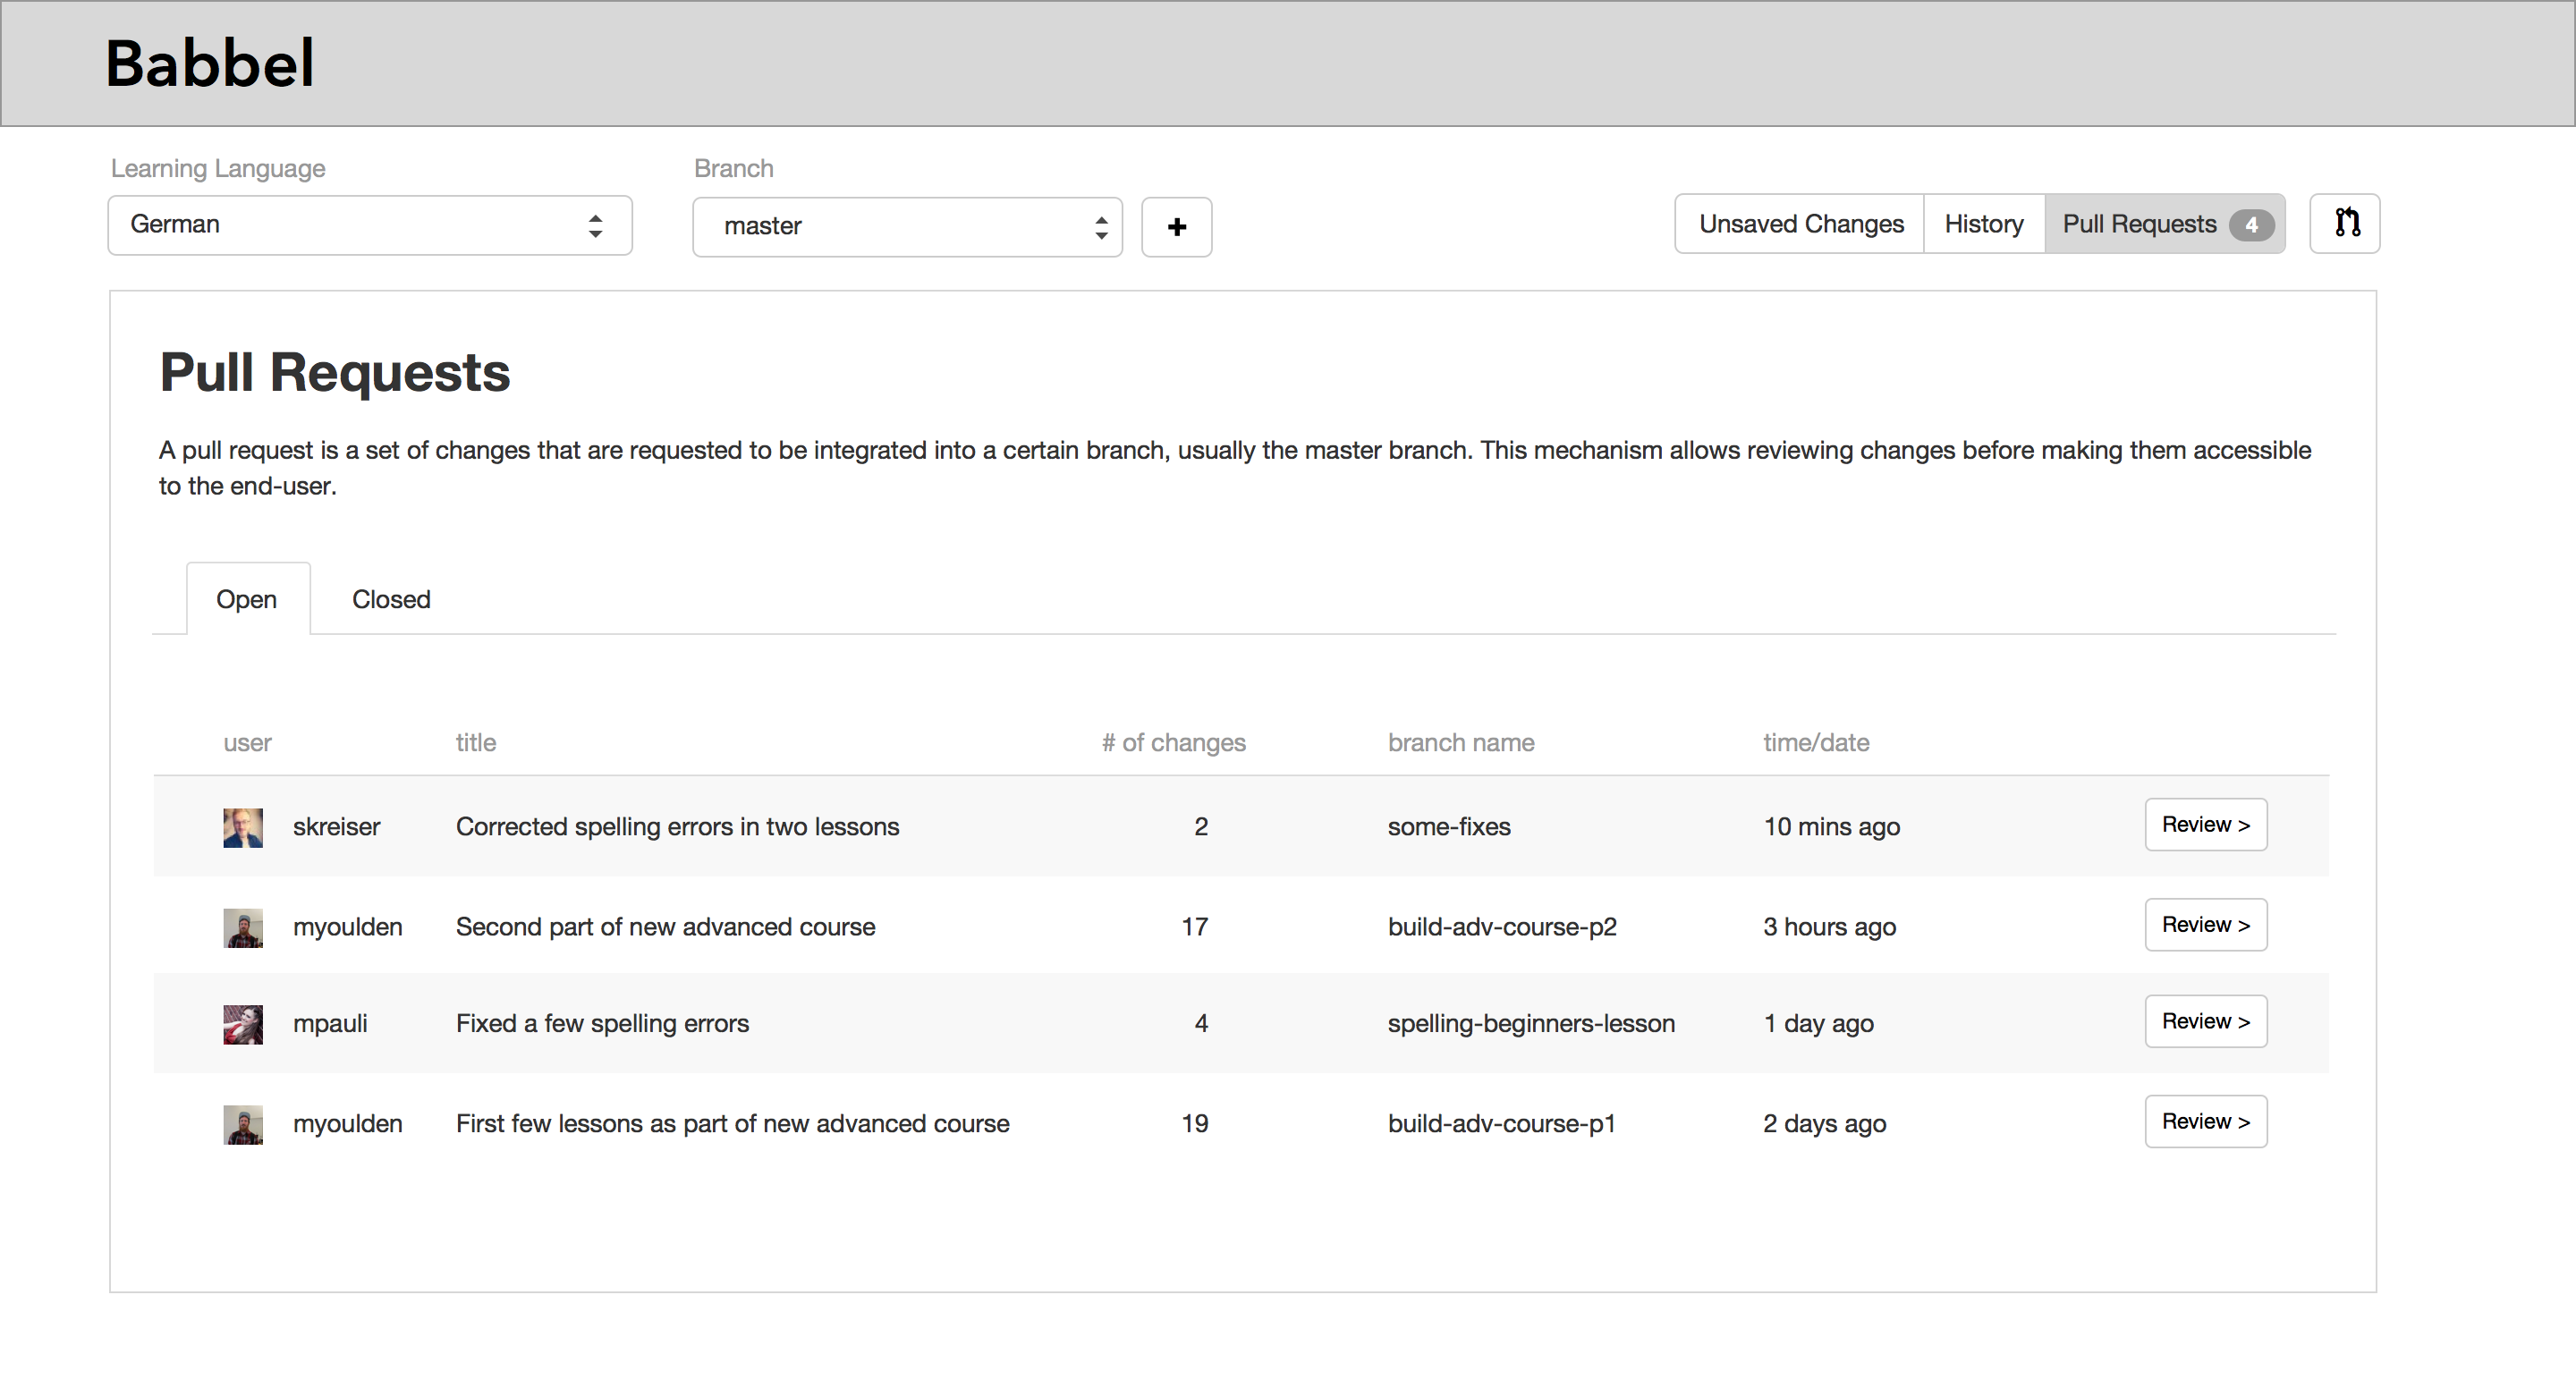
\includegraphics[width=\textwidth]{first-prototype/list-of-pull-requests}}
%  \caption{An overview of existing pull requests}
%  \label{fig:list-of-prs}
% \end{figure}

\chapter{First Usability Study} \label{chapter:first-iteration}
Using the prototype described above a task-based usability study was performed. The goal was to evaluate whether the system could be used without prior training and how well the version control workflow could be integrated into the content authoring process. The 5 participants, all full-time employees at Babbel, were first-time users of version control. 

Each session was divided into three phases. In the beginning a short pre-session questionnaire had to be answered, afterwards the participants had to perform three different tasks using the prototype and in the end an open discussion took place, during which participants could provide feedback on the interface. During each session the author was present as test moderator as well as one or two observers who took notes.

Even though the prototype was not fully functional, the study provided some valuable early feedback and revealed several usability issues (Section  \ref{sec:usability-issues-1st-study}).

\section{Study Design}
Below a more detailed description of the study design is given. The purpose of this study was to make sure that severe usability issues were discovered as early as possible in the development process.

\subsection{Participants}
The participants were recruited randomly on a first come first serve basis. All participants were full-time employees at Babbel, but some of them have also worked as freelancers for Babbel before (Table \ref{table:user-test-participants}). Most of the participants were content editors and some of them had special responsibilities, such as QA and localization. There was also one project manager who participated. This roughly reflects the distribution of content editors vs. PMs in the whole company. 

\begin{table}[h!]
\begin{tabular}{|l|l|l|p{2cm}|p{4cm}|}
\hline
\rowcolor[HTML]{EFEFEF}
{\bf Participant} & {\bf Language Team} & {\bf Job Position} \\ \hline
1 & French & Content Editor, QA \\ \hline
2 & Portuguese & Content Editor \\ \hline
3 & Portuguese & Content Editor, Localisation \\ \hline
4 & Portuguese, Spanish & Project Manager \\ \hline
5 & Turkish & Content Editor \\ \hline
\end{tabular}
\centering
\caption{List of Participants}
\label{table:user-test-participants}
\end{table}


% \section{Tested Feature Set}
% All features being tested were related to the version control capabilities of the new content authoring tool. It was important to test these, because they have not been part of the old CAT and furthermore they will be used very frequently. The list below shows which features have been tested exactly and how they are prioritized. All features were rated on a scale from 1-5 based on their importance and the level of doubt about the solutions. These numbers were then multiplied to get a total for each feature. One feature that was not included in the prototype is the resolution of merge conflicts. In theory this should be an edge case and therefore no resources were dedicated to it at this early stage of the interface.

% \begin{table}[h!]
% \begin{tabular}{|p{5cm}|l|l|l|}
% \hline
% \rowcolor[HTML]{EFEFEF}
% {\bf Feature Description}           & {\bf Importance} & {\bf Doubt} & {\bf Total} \\ \hline
% Editing and saving content          & 5                & 5           & 25          \\ \hline
% Creating pull requests              & 4                & 5           & 20          \\ \hline
% Creating and switching branches     & 5                & 4           & 20          \\ \hline
% Reviewing and merging pull requests & 4                & 4           & 16          \\ \hline
% View history of changes             & 3                & 4           & 12          \\ \hline
% \end{tabular}
% \centering
% \caption{Feature Prioritization}
% \label{table:feature-prio}
% \end{table}

%\section{Methodology}
%Below the methodology of the usability study is described in more detail. The tests were based on three different task scenarios. While users performed these tasks the test moderator as well as two observers took notes. Furthermore the sessions were recorded so that time for task completion could be measured as well as the error rate.

% here should be more about tasked-based user studies and why it was decided to do this

% \section{Test Objectives}
% There were several questions that should be answered with the user test: 

% \begin{itemize}
%   \item Evaluate whether users appreciate the separation of editing and saving or if they experience it as a burden. 
%   \item To observe how users react to the fact that they have to describe their changes when saving.
%   \item Evaluate whether the concept of a branch is understood and can be used in a meaningful way by users.
%   \item Evaluate whether users are able to use pull requests in a meaningful way.
%   \item Evaluate whether the history of changes gives users a good idea about what kind of changes happened recently.
%   \item Observe which concepts and terms confuse users the most.
% \end{itemize}

\subsection{Metrics}
Even though these quantitative measures are not statistically significant with a group of just 5 participants, they can still hint at potential problems, which should be investigated further.

% phrase it nicer, statistically significant

\begin{itemize}
  \item \emph{Successful Task Completion}: percentage of tasks that were completed successfully
  \item \emph{Time On Task}: time that was needed to perform a task
  \item \emph{Error Rate}: participant deviated from “ideal” path of navigation, such as opening the wrong menu.
\end{itemize}

%What counts as an error??

\subsection{Scenarios} \label{sec:scenario-descriptions}
As suggested by Nielsen Norman Group the tasks given to the participants were situated within real-world scenarios \cite{_task_2014}. This usually makes it easier for participants to engage with the interface in a realistic way. Furthermore, when some context is provided, the task itself does not need to be described as detailed, but rather the end-goal can be defined and the means of achieving this end-goal can be left open for the user. Three different task scenarios with an estimated duration of 4-8 minutes were created. The following task scenarios were given to the participants.

\subsubsection{Scenario 1: Fix Error and Allow Review}
A colleague (Firstname Lastname) has sent you a link to a lesson. She informed you that the second item in the vocabulary (write) exercise has the wrong speaker role (should be F1) and also should be added to the review manager. She asked you to correct the error and afterwards allow her to review your changes. Make sure you’re not editing the live content.

% \begin{itemize}
%   \item End goal: Let colleague review changes
%   \item Link: https://marvelapp.com/c89590
% \end{itemize}

\subsubsection{Scenario 2: Publish Changed Content}
A colleague (Firstname Lastname) has changed a lesson within the German language package. She asked you to review the changes. Look at the changes she made and if you don’t find any errors make them available to the Babbel end-user.

% \begin{itemize}
%   \item End goal: Publishing changed content
%   \item Link: https://marvelapp.com/1011fjj
% \end{itemize}

\subsubsection{Scenario 3: Eliminate Error and Save}
A translator (user name) is currently working on a localization of German lessons (to Portuguese). Recently a translated exercise was published, but according to customer service users have complained that there is a translation missing within this exercise. Find the exercise which has been translated and locate the item with the missing translation. Add the translation and save your changes.

\subsection{Sessions}
Each session was scheduled to take no more than 45 minutes. In the beginning every participant received a short introduction to the reasons behind the study and the procedure of the session in order to make them feel more comfortable. It was highlighted that it is not them who were being tested but the interface. Furthermore, they were encouraged to speak aloud during the tasks, especially when running into problems. At the end of each session there was a short discussion where participants could voice their concerns or name the things they liked.

\clearpage

\section{Findings}
The results below are structured in the same way the testing sessions were. First, the results of the questionnaire are presented. Then, the quantitative metrics, recorded during the sessions, are shown in four different tables. In the end, problems that became apparent when observing the participants, are listed and described in detail.

% \subsection{Pre-session Questionnaire}
% The pre-session questionnaire consisted of four different questions, that were intended to evaluate the user’s experience with version control, the current CAT and other content management or authoring systems. The table shows that no participant had prior knowledge of version control and only one had used another content management system besides the content authoring tool of Babbel. Furthermore, three out of five participants had one to three years experience with the CAT. One had less than a year of experience and one had more than three years experience. A summary of this data can be found in the appendix (Table \ref{table:pre-sess-quest}).

\subsection{Metrics}
Several quantitative metrics were gathered during the user sessions. These include completion rates, error rates and time needed for the scenarios. The metrics serve as an add-on for the mostly qualitative user studies and help to interpret the observations and findings of the test sessions.

\subsubsection{Task Completion Rate}
The table below shows a summary of how many scenarios have been successfully completed. The completion rates for Scenario 1 and Scenario 3 could hint at potential problems, which are further discussed below.

\begin{table}[h!]
\begin{tabular}{|l|l|l|l|}
\hline
\rowcolor[HTML]{EFEFEF} 
{\bf User}                     & {\bf Scenario 1} & {\bf Scenario 2} & {\bf Scenario 3} \\ \hline
1                              & no           & yes          & yes          \\ \hline
2                              & yes          & yes          & yes          \\ \hline
3                              & yes          & yes          & no           \\ \hline
4                              & no           & yes          & no      \\ \hline
5                              & no      & yes          & yes          \\ \hline
\rowcolor[HTML]{EFEFEF} 
Success & 2 & 5 & 3 \\ \hline
\rowcolor[HTML]{EFEFEF} 
{\bf Completion Rate} & {\bf 40\%}   & {\bf 100\%}  & {\bf 60\%}   \\ \hline
\end{tabular}
\centering
\caption{Task completion rate}
\label{table:task-completion-rate}
\end{table}

\subsubsection{Time on Task}
The time on task was measured based on the video recordings of the sessions. The large differences between Scenario 2 and the other scenarios might be due to the different levels of difficulties inherent to the tasks presented in the scenarios. The table below highlights the shortest and longest times that were needed to finish a certain scenario. The times for Scenario 1 have the highest variance, which could point towards potential usability problems which were not encountered by all users. Scenario 1 asked users to “not edit the live data”, which meant that they had to create a new branch. Since none of the participants had prior experience with version control, this was a particularly difficult scenario for some of them. 

\begin{table}[h!]
\begin{tabular}{|r|r|r|r|r|r|r|r|}
\hline
\rowcolor[HTML]{EFEFEF} 
{\bf Scenario} & \multicolumn{1}{c|}{\cellcolor[HTML]{EFEFEF}{\bf User 1}} & {\bf User 2} & {\bf User 3} & {\bf User 4} & {\bf User 5} & {\bf Mean} & {\bf Var} \\ \hline
\cellcolor[HTML]{EFEFEF} 1 & 505 & 270 & 313 & 275 & 519 & 376 & 15624 \\ \hline
\cellcolor[HTML]{EFEFEF} 2 & 81 & 226 & 73 & 170 & 90 & 128 & 4511 \\ \hline
\cellcolor[HTML]{EFEFEF} 3 & 301 & 375 & 418 & 507 & 399 & 400 & 5550      \\ \hline
\end{tabular}
\centering
\caption{Time needed to perform scenarios (in seconds)}
\label{table:time-on-tasks}
\end{table}

\subsubsection{Error Rates}
An interaction was counted as an error if the user departed from the ideal path and thus the interaction did not contribute to solving the overall goal of the scenario. The table below helps to paint a picture of how much trial and error was necessary. The error rate is not necessarily a sign for bad usability, it can also reflect the difficulty of a scenario. For example, Scenario 1 and 3 involved using similar parts of the interface, but Scenario 3 challenged a participant's mental model of the system whereas Scenario 1 was a little more straightforward. 

% explain how mental model was challenged

\begin{table}[h!]
\begin{tabular}{|r|r|r|r|r|r|r|r|}
\hline
\rowcolor[HTML]{EFEFEF} 
\multicolumn{1}{|l|}{\cellcolor[HTML]{EFEFEF}{\bf Task}} & \multicolumn{1}{l|}{\cellcolor[HTML]{EFEFEF}{\bf User 1}} & \multicolumn{1}{l|}{\cellcolor[HTML]{EFEFEF}{\bf User 2}} & \multicolumn{1}{l|}{\cellcolor[HTML]{EFEFEF}{\bf User 3}} & \multicolumn{1}{l|}{\cellcolor[HTML]{EFEFEF}{\bf User 4}} & \multicolumn{1}{l|}{\cellcolor[HTML]{EFEFEF}{\bf User 5}} & \multicolumn{1}{l|}{\cellcolor[HTML]{EFEFEF}{\bf Mean}} & \multicolumn{1}{l|}{\cellcolor[HTML]{EFEFEF}{\bf Var}} \\ \hline
\cellcolor[HTML]{EFEFEF}1                                & 3                                                         & 1                                                         & 3                                                         & 3                                                         & 1                                                         & 2.2                                                     & 0.96                                                   \\ \hline
\cellcolor[HTML]{EFEFEF}2                                & 0                                                         & 5                                                         & 0                                                         & 3                                                         & 0                                                         & 1.6                                                     & 4.24                                                   \\ \hline
\cellcolor[HTML]{EFEFEF}3                                & 3                                                         & 6                                                         & 7                                                         & 3                                                         & 2                                                         & 4.2                                                     & 3.76                                                   \\ \hline
\end{tabular}
\centering
\caption{Number of errors done by each participant}
\label{table:error-rate}
\end{table}

%\subsubsection{Summary of Quantitative Data}

%\begin{table}[h!]
%\begin{tabular}{|r|r|r|r|r|}
%\hline
%\rowcolor[HTML]{EFEFEF} 
%\multicolumn{1}{|l|}{\cellcolor[HTML]{EFEFEF}{\bf Task}} & \multicolumn{1}{l|}{\cellcolor[HTML]{EFEFEF}{\bf Completed}} & \multicolumn{1}{p{2cm}|}{\cellcolor[HTML]{EFEFEF}{\bf Task completion rate}} & \multicolumn{1}{l|}{\cellcolor[HTML]{EFEFEF}{\bf Errors (mean)}} & \multicolumn{1}{p{2cm}|}{\cellcolor[HTML]{EFEFEF}{\bf Time (sec) (mean)}} \\ \hline
%\cellcolor[HTML]{EFEFEF}1                                & 2                                                            & 40\%                                                                    & 2.2                                                              & 376.4                                                                        \\ \hline
%\cellcolor[HTML]{EFEFEF}2                                & 5                                                            & 100\%                                                                   & 1.6                                                              & 128                                                                          \\ \hline
%\cellcolor[HTML]{EFEFEF}3                                & 3                                                            & 60\%                                                                    & 4.2                                                              & 400                                                                          \\ \hline
%\end{tabular}
%\centering
%\caption{ Summary of quantitative data collected}
%\label{table:quant-data-summary}
%\end{table}

\subsection{Discovered Usability Issues} \label{sec:usability-issues-1st-study}
The following section describes the usability issues that have been discovered by observing participants performing the different scenarios. In total, 26 different problems were identified. 7 of them were so severe they prevented participants from finishing their tasks. 8 issues caused a significant delay or frustration for users. The remaining issues only caused minor problems or were suggestions for improvement.

In order to rank the issues by their impact on the user experience a severity score was used, as suggested by Sauro and Lewis \cite{sauro_quantifying_2012}. The most severe issues, which prevented users from completing the tasks, were given a score of 10. 5 points were assigned if the issue caused a significant delay or frustration. 3 points were allocated for minor issues and just 1 point for improvements suggested by participants. To create an impact score the severity was multiplied by the frequency of users who experienced the problem (severity * frequency / 10). A frequency of 40\% means that 4 of 10 users encountered the problem, independent of whether they ran into the issue more than once. The scale ranges from 100 (most severe problem, experienced by all users) to 1 (suggestion by a single user). 

The issues below are grouped by feature areas and ranked by their impact on the user experience. The most impactful issues are shortly explained. 

%Link to complete list of problems in appendix?

\subsubsection{Branches}
As can be seen in Table \ref{table:issues-branches} one of the most impactful usability issues was the difficult discovery of the branch creation functionality (Issue \#1). During Scenario 1, 3 out of 5 participants spent more than half of the time by searching for this feature. Figure \ref{fig:branch-creation-time} visualizes this fact. The dark bars mark the point in time when users discovered the branch creation feature. The problem might have been a missing label for the button, which only consisted of a plus sign. Apparently, the proximity to the branch dropdown as well as the tooltip appearing upon hovering the button, did not suffice to make this feature discoverable.

There were two more issues with a severity score of 10. Issue \#2: Some users dismissed the master branch warning (without reading it), which lead to even more confusion and prevented some of them from finishing the task. 

The remaining issues highlight that the concept of a branch was only poorly understood (Issue \#3) and that the naming of the default branch (master) is rather unfortunate (Issue \#4), because it interferes with a different concept (master language) that describes the main translation language. 

\begin{table}[h!]
\centering
\begin{tabular}{|l|p{7cm}|l|l|l|}
\hline
\rowcolor[HTML]{EFEFEF} 
\textbf{\#} & \textbf{Usability issue} & \textbf{Severity} & \textbf{Frequency} & \textbf{Impact} \\ \hline
1 & Create new branch button was not found & 10 & 40\% & 40 \\ \hline
2 & Warning about editing content inside the master branch was ignored & 10 & 40\% & 40 \\ \hline
3 & It is not clear that the master branch represents the public content and the content in all other branches is not visible to the end-user. & 5 & 60\% & 30 \\ \hline
4 & The naming for the master branch was confused with the concept of a master language. & 5 & 40\% & 20 \\ \hline
5 & After creating branch it is not clear that system switched to new branch already & 5 & 20\% & 10 \\ \hline
\end{tabular}
\caption{Usability problems related to branches}
\label{table:issues-branches}
\end{table}

\begin{figure}[h!]
 \centering
 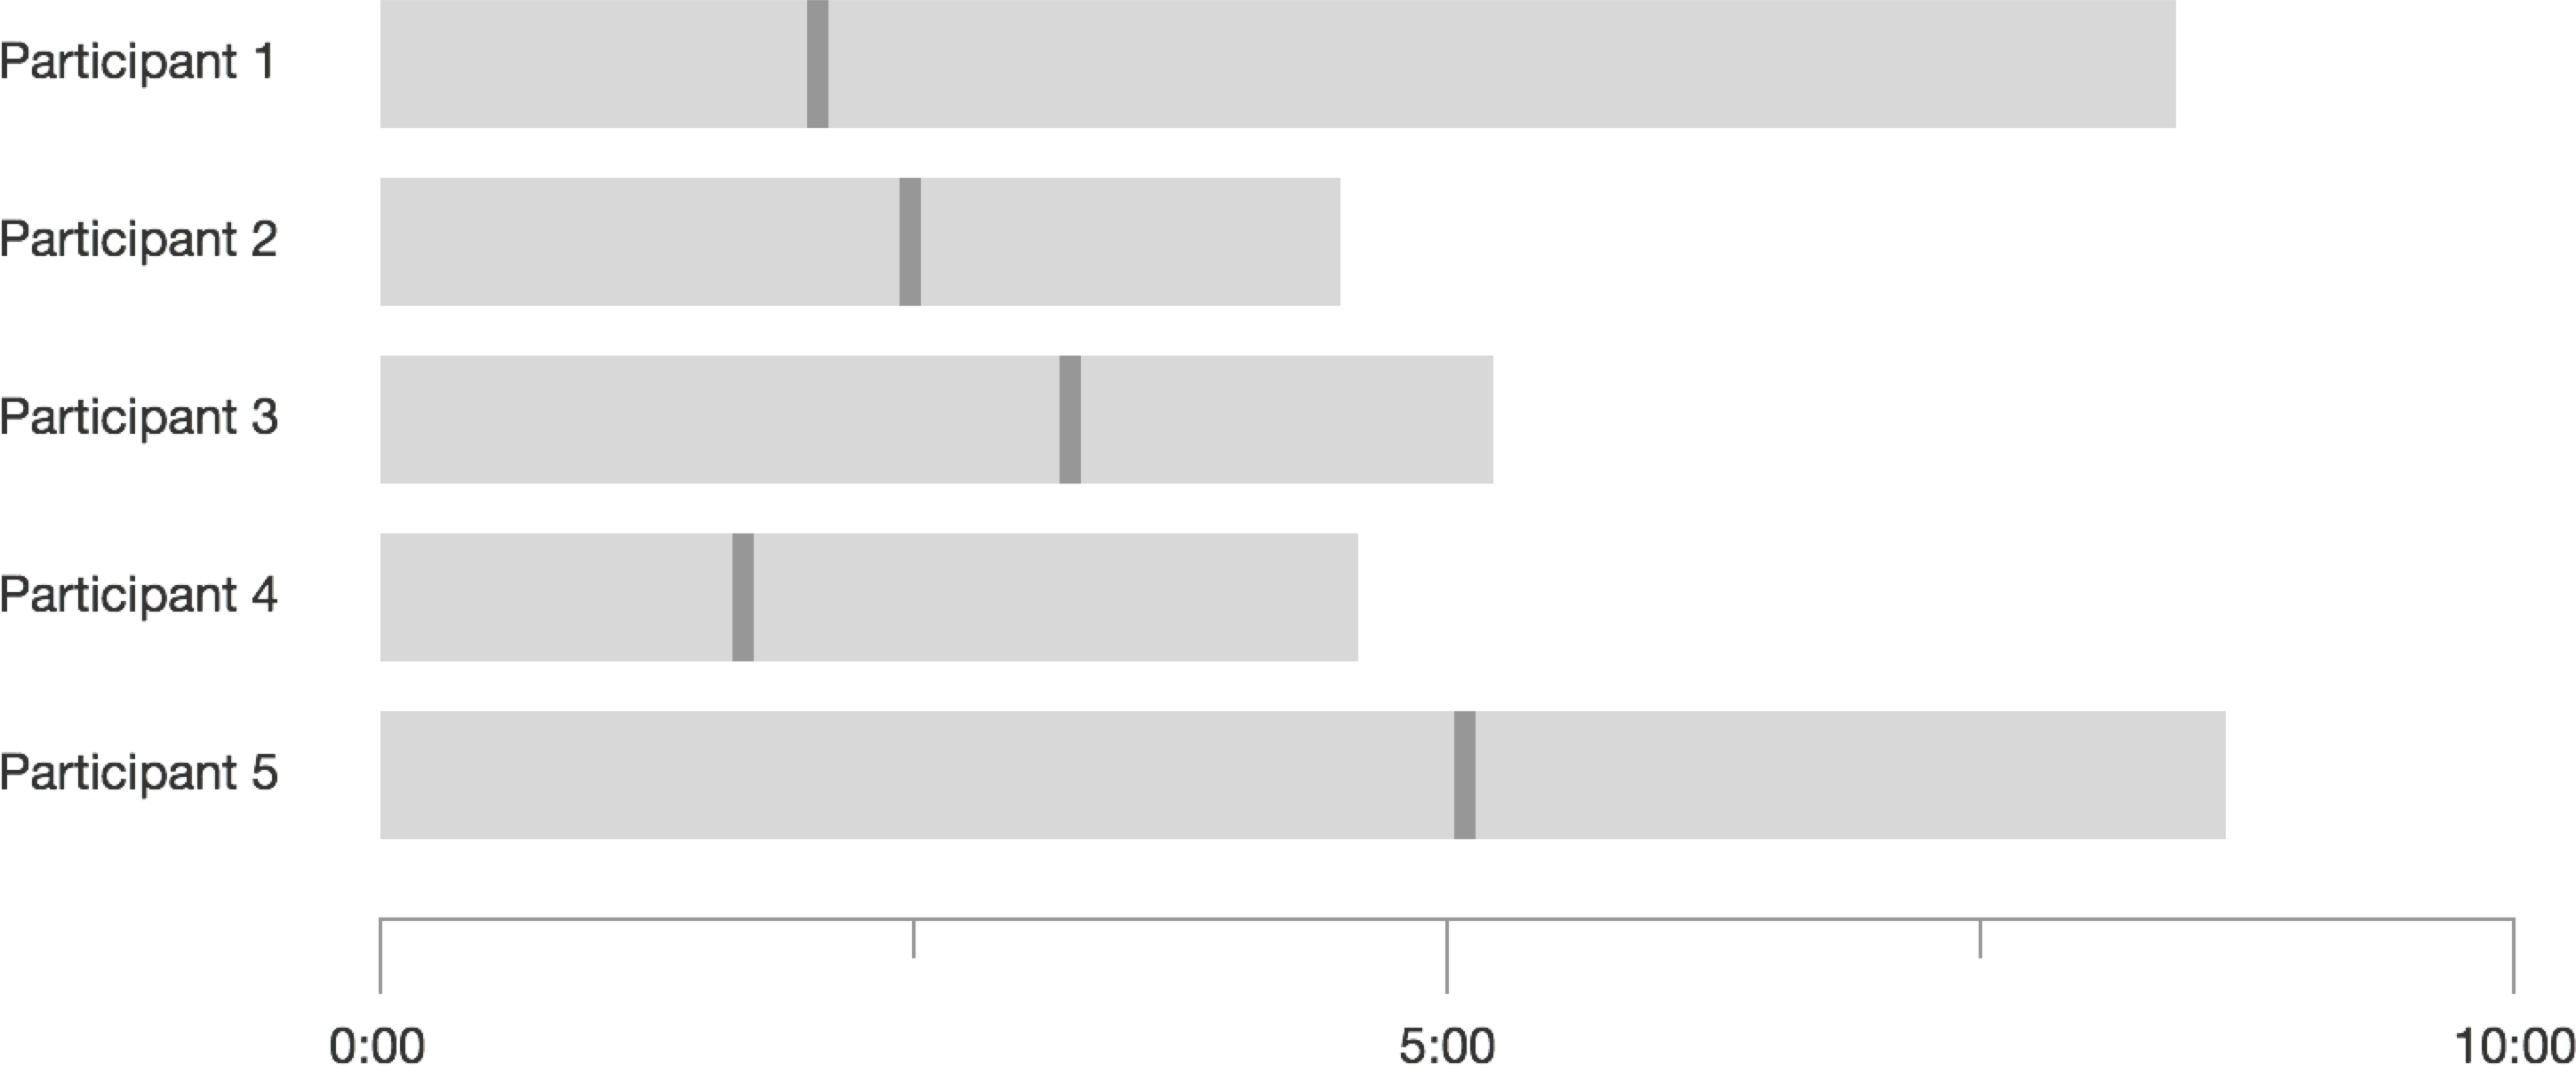
\includegraphics[width=12cm]{plot-time-till-branch-creation}
 \caption{Total task completion time compared to discovery of branch creation button}
 \label{fig:branch-creation-time}
\end{figure}

\subsubsection{Pull Requests}
Pull requests are similar to branches in that they are one of the most complex concepts in version control. As suspected, they caused a couple of usability problems. The most important issue was related to the naming: deriving the functionality of a pull request just from its name is almost impossible (Table \ref{table:issues-pull-requests}, Issue \#6). When using a Git CLI the \emph{pull} command fetches changes from the remote repository and merges them into the local repository. Therefore, a pull request describes a request to "pull a new set of changes". But since this command is not exposed to users inside the GUI of the content authoring tool, it is fairly difficult for them to guess what kind of functionality is concealed behind this name.

\begin{table}[h1]
\centering
\begin{tabular}{|l|p{7cm}|l|l|l|}
\hline
\rowcolor[HTML]{EFEFEF} 
\textbf{\#} & \textbf{Usability issue} & \textbf{Severity} & \textbf{Frequency} & \textbf{Impact} \\ \hline
6 & Concept of a pull request is not clear (term might be confusing) & 5 & 80\% & 40 \\ \hline
7 & Some users missed the reviewer field & 10 & 20\% & 20 \\ \hline
8 & Confused pull request title with lesson title & 5 & 20\% & 10 \\ \hline
9 & Branch visualization is unclear (release branch) & 3 & 20\% & 6 \\ \hline
10 & Changes vs. Overview unclear (pull request detail view) & 3 & 20\% & 6 \\ \hline
\end{tabular}
\caption{Usability issues related to Pull Requests}
\label{table:issues-pull-requests}
\end{table}

\subsubsection{Diff}
During Scenario 3, a high proportion of users had problems comprehending the list of changes presented to them (Table \ref{table:issues-diff}, Issue \#11). In general, the diff view worked well, but when asked to find a missing translation, most users had a hard time understanding that something that had not been changed, would not appear in the diff view. Furthermore, the list of changes they did see, was confusing, because it showed empty fields, which some users mistook as the missing translation they were supposed to find (Figure \ref{fig:add-translation-diff}). 

\begin{figure}[h!]
 \centering
 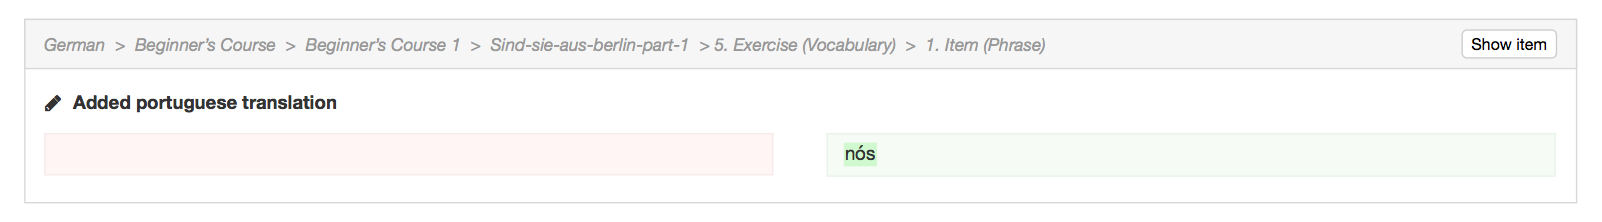
\includegraphics[width=\textwidth]{first-prototype/add-translation-diff}
 \caption{Part of diff view that displays an added translation}
 \label{fig:add-translation-diff}
\end{figure}

\begin{table}[h!]
\centering
\begin{tabular}{|l|p{7cm}|l|l|l|}
\hline
\rowcolor[HTML]{EFEFEF} 
\textbf{\#} & \textbf{Usability issue} & \textbf{Severity} & \textbf{Frequency} & \textbf{Impact} \\ \hline
11 & New translations listed in the diff view are confusing, because the left column is empty (some users expected to see the learning language text) & 10 & 80\% & 80 \\ \hline
12 & Not clear how to get from the diff view to the editing view & 10 & 40\% & 40 \\ \hline
13 & red and green are confusing as colors (red is associated with a mistake) & 3 & 20\% & 6 \\ \hline
\end{tabular}
\caption{Usability issues related to the diff view}
\label{table:issues-diff}
\end{table}


\subsubsection{Saving Process}
The most problematic issue related to saving was the non-existing save button at the bottom of the view (Table \ref{table:issues-saving-process}, Issue \#14). Most users overlooked the saving feature in the navigation bar. It seems like most users would rather expect it to be attached to the lesson editor itself. The reason it is at the top is that saving is independent of content itself. In theory, several lessons could be edited and then only saved in the end altogether. This approach is very similar to how version control usually works, but it did not seem to resonate with most users. Many were anxious to navigate away from the current view after doing changes, because they feared of losing the changes. In most interfaces, saving is directly associated with a change that was done before. A solution needs to be found that is less counter-intuitive, but which still offers users a way of reviewing what was changed.

\begin{table}[h!]
\centering
\begin{tabular}{|l|p{7cm}|l|l|l|}
\hline
\rowcolor[HTML]{EFEFEF} 
\textbf{\#} & \textbf{Usability issue} & \textbf{Severity} & \textbf{Frequency} & \textbf{Impact} \\ \hline
14 & Save button was not found (expected at bottom of screen) & 10 & 80\% & 80 \\ \hline
15 & Expects saved changes to be public right away & 10 & 20\% & 20 \\ \hline
16 & Confused back-to-editor-button with review functionality & 5 & 40\% & 20 \\ \hline
17 & Wording on saved changes confirmation page is somewhat confusing & 3 & 20\% & 6 \\ \hline
18 & Concept of separated saving not entirely clear (across lessons) & 3 & 20\% & 6 \\ \hline
\end{tabular}
\caption{Usability issues related to the saving process}
\label{table:issues-saving-process}
\end{table}

% \subsubsection{History}
% \begin{table}[h!]
% \centering
% \begin{tabular}{|p{7cm}|l|l|l|}
% \hline
% \rowcolor[HTML]{EFEFEF} 
% \textbf{Usability Issue} & \textbf{Severity} & \textbf{Frequency} & \textbf{Impact} \\ \hline
% History is not recognized for what it is. Most users take long to find it. (naming might not be obvious) & 5 & 40\% & 20 \\ \hline
% Difference between pull request and history not entirely clear & 3 & 20\% & 6 \\ \hline
% Change of a specific user is not found – search functionality suggested & 3 & 20\% & 6 \\ \hline
% \end{tabular}
% \caption{Usability issues related to the saving process}
% \label{table:issues-saving}
% \end{table}

\subsubsection{Main Editing View}
The main editing view only caused a couple of minor problems. First and foremost, the way the content was structured and presented to the user was not the most intuitive (Table \ref{table:issues-editing-view}, Issue \#19). Most users struggled with envisioning how the representation would translate into the actual exercises provided to the Babbel end-user. Additionally, the design did not provide a very good overview, because every exercise or item had to be expanded and at any given moment one could only see one at most.

The remaining issues were suggestions (Issue \#21 \& Issue \#22) or related to the visual design of the interface (Issue \#20).

\begin{table}[h!]
\centering
\begin{tabular}{|l|p{7cm}|l|l|l|}
\hline
\rowcolor[HTML]{EFEFEF} 
\textbf{\#} & \textbf{Usability issue} & \textbf{Severity} & \textbf{Frequency} & \textbf{Impact} \\ \hline
19 & Visual representation/hierarchy of items/exercises not entirely clear & 3 & 60\% & 18 \\ \hline
20 & Learning language text is overlooked (looks different than translations) & 3 & 20\% & 6 \\ \hline
21 & Suggested a search functionality to find content faster & 1 & 40\% & 4 \\ \hline
22 & Suggested pro-active system for translations & 1 & 20\% & 2 \\ \hline
\end{tabular}
\caption{Usability issues related to the main editing view}
\label{table:issues-editing-view}
\end{table}


\subsubsection{Miscellaneous}
In addition to the issues related to the major feature areas a couple of miscellaneous problems appeared throughout the system. None of the issues was of the highest severity, but they still caused some frustration. Especially Issues \#23 and \#25 reduced the smoothness with which users could move through the system. It seems that the naming for some of the navigation items was not descriptive enough and that icons without a label were more or less ignored. Some users proceeded by trial and error, which does not speak for the clarity of the information architecture. 

\begin{table}[h!]
\centering
\begin{tabular}{|l|p{7cm}|l|l|l|}
\hline
\rowcolor[HTML]{EFEFEF} 
\textbf{\#} & \textbf{Usability Issue} & \textbf{Severity} & \textbf{Frequency} & \textbf{Impact} \\ \hline
23 & Main navigation not completely obvious, clicking through (trial \& error) & 5 & 40\% & 20 \\ \hline
24 & History is not recognized for what it is. Most users take long to find it. (naming might not be obvious) & 5 & 40\% & 20 \\ \hline
25 & Navigation: Icons without text are not understood "What is this?" (pull request icon) & 3 & 20\% & 6 \\ \hline
26 & No help offered when needed & 1 & 20\% & 2 \\ \hline
\end{tabular}
\caption{Miscellaneous usability issues}
\label{table:issues-misc}
\end{table}


% \subsubsection{Scenario 1}
% Scenario 1 asked participants to fix two errors in a lesson, save the changes and enable a colleague to review the changes before making them public. Translated into the version control world this corresponds to creating a branch, editing, staging and committing the changes and finally creating a pull request. 

%The first step, creating a new branch, seemed to be the major hurdle for most participants. Even though it was basically the first thing that users had to do, 3 out of 5 participants needed more than half of the total task completion time for discovering this feature. Figure \ref{fig:branch-creation-time} visualizes this fact. The dark bars mark the point in time when users discovered the branch creation feature.

% \begin{figure}[h!]
%  \centering
%  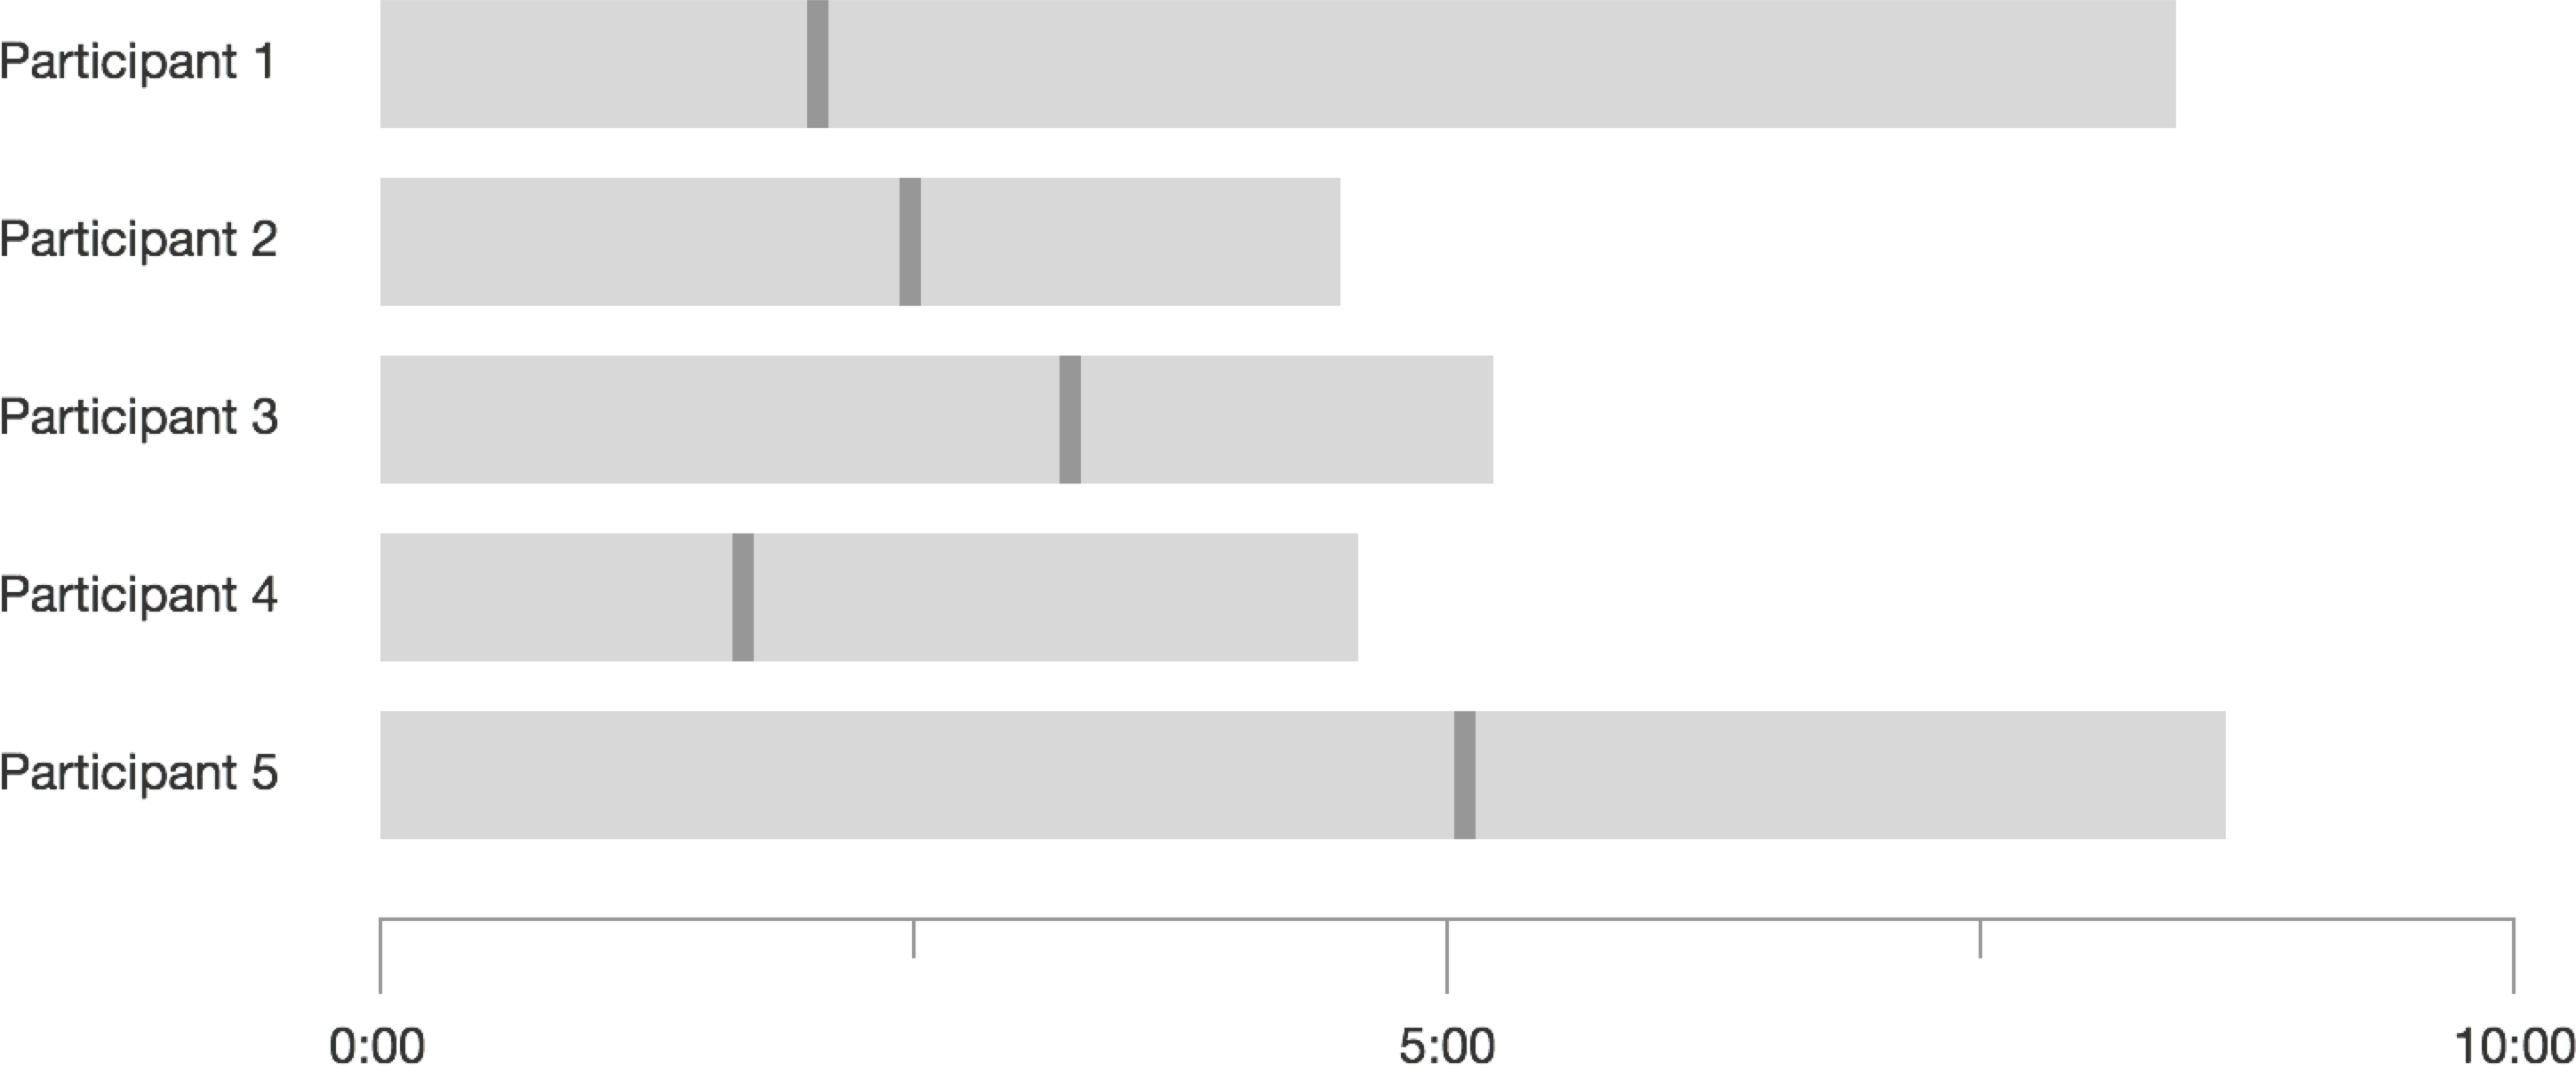
\includegraphics[width=\textwidth]{plot-time-till-branch-creation}
%  \caption{Total task completion time compared to discovery of branch creation button}
%  \label{fig:branch-creation-time}
% \end{figure}

% One factor that lead to this situation was that most users did not fully read the warning message, which told them they could not edit the main branch, but instead had to create a new one. The second factor, it seemed, was the missing label for the button that allowed the creation of a new branch. The button only consisted of a simple plus sign and a tooltip would explain more if the user hovered the button (Figure \ref{fig:create-new-branch-btn}). Some users, after exhausting all other options, turned to the last available option. Others accidentally hovered the button and thus discovered the feature.

% \begin{figure}[h!]
%  \centering
%  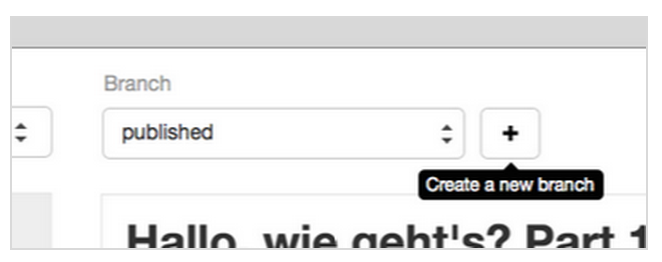
\includegraphics[width=6cm]{create-new-branch}
%  \caption{The branch selection next to the create-new-branch button}
%  \label{fig:create-new-branch-btn}
% \end{figure}

% Another problem was that some participants could not figure out how they could allow a colleague to review their edits. This is also reflected in the task completion percentage shown in Table \ref{table:task-completion-rate}. This issue seemed to be connected to bad naming (some users misinterpreted the \textit{back to editor button}) and an overlooked input field (\textit{reviewer} on pull request view). Furthermore, one user had a wrong mental model of the system in that she assumed the colleague who sent her the link would be informed about changes automatically. 

% \subsubsection{Scenario 2}
% This scenario presented almost no problems to the participants. This is reflected by the low error rate, the short time needed for performing the tasks and the 100\% completion rate (Table \ref{table:task-completion-rate}). The three users who made zero errors while performing the tasks were drawn to the pull request view by the number indicator next to the button (Figure \ref{fig:number-indicator-pr}). The other two users struggled, because the concept of a pull request was meaningless to them, even though one of them had created one during the previous scenario. Both started by selecting folders in the main navigation and then went on to discover the right functionality through trial and error (“I have no idea, I’m just clicking through”). Once these users discovered the pull request view they were able to finish the task without major problems like the other participants. 

% \begin{figure}[h!]
%  \centering
%  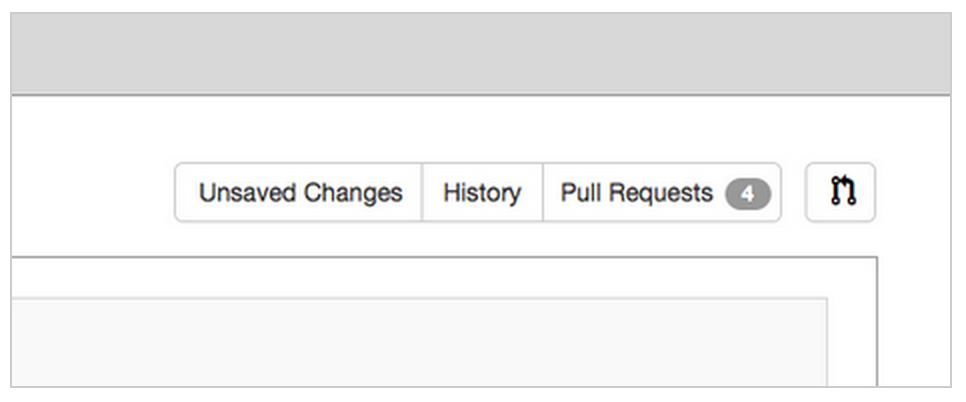
\includegraphics[width=9cm]{number-indicator-pr}
%  \caption{Number indicator next to the pull request button}
%  \label{fig:number-indicator-pr}
% \end{figure}

% \subsubsection{Scenario 3}
% This scenario, out of all scenarios, challenged participants the most. This can be seen in the high error rates (4.2 on average) and the time needed for completing the scenario, which was the highest of all scenarios. The first obstacle users encountered was that the changes could not be found in the list of pull requests as in the previous scenario, but instead in the history. During the post-session interviews some users stated, that the difference between the two was not clear. This could be due to the similarity of the two concepts. The history is a list of saved changes whereas a pull request is a request to integrate a set of changes into a different branch. But both are lists of changes, which could explain the confusion. 

% The second major problem, which was even more severe, was that most users struggled to find the missing translation. This was partly due to confusion that was caused by the difference view (Figure \ref{fig:difference-view}). Users mistook the left column, which represents the old state of the data, for the missing translations. The other contributing factor was that users had to make an abstraction from the difference view to the list of items that were presented to them inside the editing view (Figure \ref{fig:missing-translation}). Those users that solved the task realized that a missing translation would not show up in the list of changes and thus they had to use the editing view to navigate to the respective item. User who did not complete the task (2 of 5) failed to make this connection.

% \begin{figure}[h!]
%  \centering
%  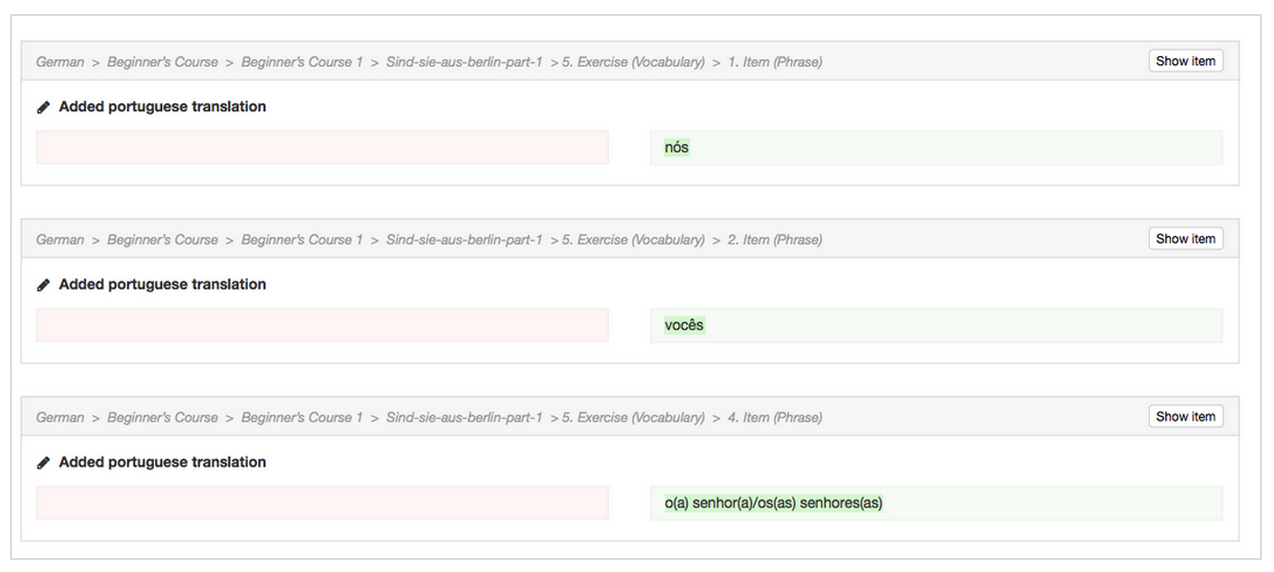
\includegraphics[width=\textwidth]{difference-view}
%  \caption{Difference view as presented to the user when inspecting changes}
%  \label{fig:difference-view}
% \end{figure}

% \begin{figure}[h!]
%  \centering
%  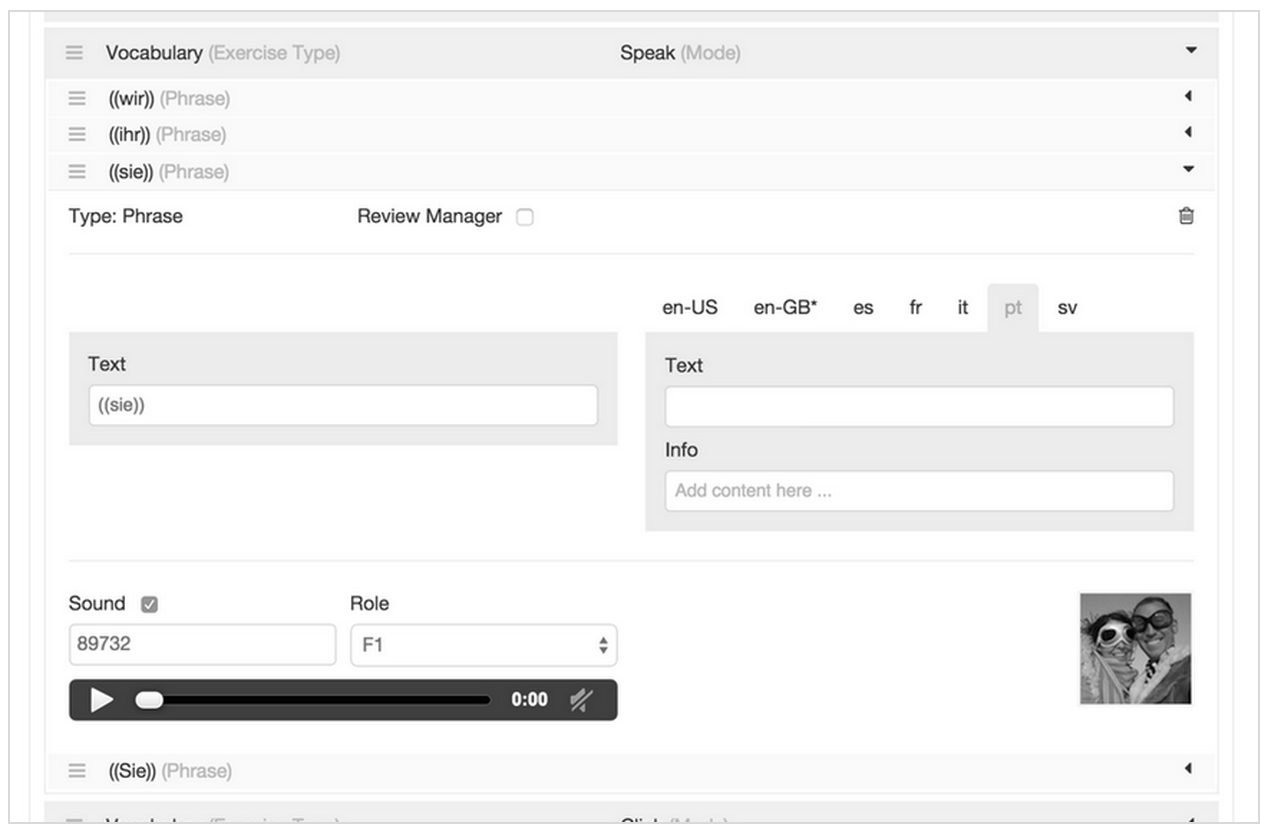
\includegraphics[width=\textwidth]{missing-translation}
%  \caption{Expanded item with missing translation}
%  \label{fig:missing-translation}
% \end{figure}

% I left out the recommendations/possible solutions -> maybe they could become part of each scenario?

\subsection{Conclusion} \label{sec:summary-usability-problems}
Concluding one could say that a long list of diverse usability issues has been identified. A number of severe issues prevented users from finishing their tasks, especially in Scenarios 1 and 3. This is also reflected in the somewhat low task completion rates for these scenarios. 
Furthermore, using central features, such as branching and saving posed some serious problems, which reflected on the entire system. Last but not least, the use of technical terminology (e.g. branch or pull request) prevented some users from forming an accurate mental model of the system. But, despite these flaws, a majority of users still succeeded in reaching their goals, which is more important than having an accurate understanding of the underlying concepts, which will probably improve over time. 

Nevertheless, there are many things that need to be improved for the next iteration of the interface. The following chapter looks at one aspect of that: the terminology used within the interface. After that, Chapter \ref{chapter:design-second-iteration} presents how the discovered issues were resolved and translated into a new interface design. 


%During Scenario 1, especially the first part, creating a new branch, was a difficult hurdle for almost all users. This might be due to the fact that this approach was completely new to all participants, since none of them had used version control before. This problem was further intensified by the fact that users did not fully read the warning popup. 

%Solutions for this problem, as described in the section above, are rephrasing the warning or offering a direct link to the branch creation view. 

%Another issue, that most users had, is the separation of editing and saving. Even though some users stated that it is advantageous to get an overview of changes before saving, all of them were looking for a save button at the bottom of the editing view. It took them a while to locate the “unsaved changes” button at the top. The decoupling of saving and editing is an important feature that allows bundling changes into a coherent edit (which makes the history more valuable). Therefore, in order to keep this feature, a compromise needs to be found between offering users a familiar save and edit workflow while at the same time providing them the enhanced VCS capabilities.

%A big question mark is still how users can be introduced to the more complex version control features. During the post-session interviews it became clear that most participants had no real understanding of branches or pull requests. Furthermore, the difference between history and pull requests was not really clear. 


%Nevertheless, a better understanding could probably be achieved through an improved naming instead of just using the existing Git terminology.

% \subsection{Recommendations}
% Based on the results of this user study a few recommendations were drafted. These acted as broad guidelines for the design of the next prototype.

% \begin{itemize}
%   \item Offer a short interactive tutorial that introduces new users to the most important version control concepts
%   \item There should be a direct path from the master branch warning to the branch creation view (or at least a better description: “create a new branch first” could be the headline for example)
%   \item Button order should reflect temporal sequence in which functions are used: branch creation/selection - saving changes - getting an overview of changes (history) - merging branches
%   \item Offer a save button at the bottom of the editing view which either leads to the unsaved changes view or lets users save without reviewing the changes again (lesson based)
%   \item Names for the most important features could be reconsidered (Focus Group)
%   \item Item list should be numbered
%   \item Evaluate whether providing more context within change overview is feasible (images, speaker role)
%   \item Highlight which item actually is selected, what changed (after coming from the change overview)
% \end{itemize}




\chapter{Focus Group} \label{chapter:focus-group}
As the previous usability study has shown, the naming of features was a major usability issue. Participants have been exposed to entirely new concepts. Errors that have been made during the sessions were often related to a misunderstanding of what a feature does. How things are phrased influences a user’s comprehension of a system, his or her mental model, strongly. As described in Chapter \ref{chapter:related-work} Git's conceptual model is flawed in certain ways, which is also reflected in its terminology. In order to avoid adopting these flaws for the content authoring tool, some Git concepts had to be revised, reconsidered or combined. This is why new names needed to be found for these concepts, which would properly reflect their purpose and help users to form an accurate mental model. The goal of the focus group was to identify those concepts that are particularly problematic as well as ideating on better names. The expected outcome were new ideas as well as valuable input for the second design iteration.

%In the tradition of co-operative design \cite{ehn_cooperative_2000} a workshop was held including the participants of the first usability study as well as the team working on the content authoring tool.

% talk a bit about co.design?

%write how this was also about identifying what the difficult terms are -> more focus on discovery and getting insights than on generating new ideas

%\section{Objectives}
%First and foremost the focus group is intended to provide a better understanding of the user’s thought process. Which terms are hard to understand or even misleading? Can they derive a function’s purpose based on its name? Since the participants were already exposed to the terms and corresponding features they will be able to provide feedback based on their own experience. Besides gaining insights the focus group also aims at producing suggestions for improvements. How can terms be rephrased to allow an easier understanding?

\section{Procedure}
The focus group was scheduled for max. 90 minutes with a short break in between. The first part consisted of an open discussion among the participants, during which they talked about their difficulties during the testing sessions. They were briefed to put particular emphasis on the language used within the interface. In case the discussion steered off into another direction, the author, who acted as the facilitator, tried to direct it to the terminology aspect again.

During the second phase, participants were expected to come up with alternatives for the current naming. In a short survey, prior to the meeting, participants had voted which features and terms they found most puzzling (See below). The results of the survey as well as the outcome of the previous usability study, formed the basis for the discussions during the second phase. In order to provide participants with a more solid understanding of version control, a short presentation was given before the start of the second phase. Afterwards participants were asked to conceive alternatives for the most problematic terms. At first for themselves and later on together with their peers.

\section{Most Problematic Terms}
In a short survey prior to the meeting participants had been asked how well they had understood different version control concepts. The 5 least understood terms or features are listed below. Most of them evolve around pull requests, branching and merging. Furthermore, the previous usability study had shown that naming of the default branch ("master branch", Issue \#4) and the history (Issue \#24) can cause problems as well.

\begin{itemize}
 \item Pull Request
 \item Create (Pull Request)
 \item Branch
 \item Merge
 \item Reviewer
\end{itemize}

\section{First Phase}
The first phase, the open discussion, showed that still a lot of confusion prevailed among the participants regarding the most common version control concepts. It is hard to say whether this is because of the names used for these concepts or because the concepts are inherently hard to understand. Branch and pull request, for example, seemed to be most problematic, but they are also conceptually the most complex. One of the participants even thought they are more or less the same thing. Another one mentioned, she could not tell the difference between the three concepts of unsaved changes, history and pull requests and had no idea in which order to use them. To conclude, one could say, that none of the participants (except for one) had formed an accurate mental model of the system, which is not surprising, given that they have only used it once and were not introduced to it before.

The participants agreed that it is easier to understand the concepts once they are explained, but they also stated that freelancers likely will not have this luxury. Most people agreed that illustrations, explanations and tooltips can be a great help while using the system.

% \begin{figure}[h!]
%  \centering
%  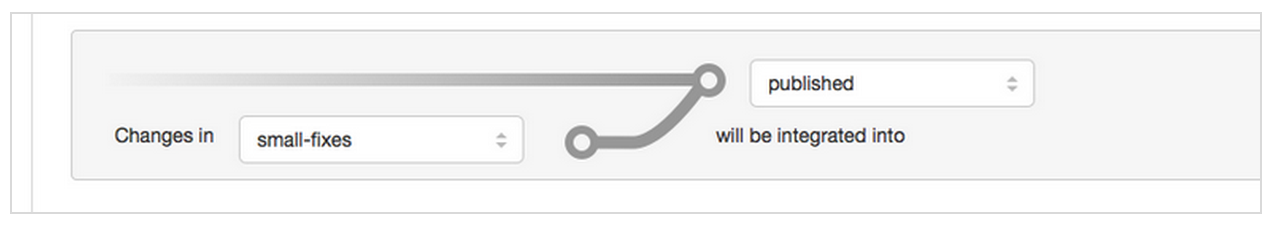
\includegraphics[width=\textwidth]{branch-visualization}
%  \caption{Illustration that visualizes what happens when two branches are merged}
%  \label{fig:branch-visualization}
% \end{figure}

\section{Second Phase}
At the beginning of the second phase the author gave a short introduction to version control and the most important concepts. This was done to provide the participants with a solid understanding of version control and its concepts, thus making it easier for them to come up with alternative names. The brainstorming proved to be more difficult than expected, but yielded a handful of alternative terms for each concept that had been deemed hard to comprehend earlier. What made it difficult to find different names for some concepts was the large domain they have to work for. For example, a translator creates a pull request in order to request proofreading, but one can not name it “request proofread”, because for some users it serves a different purpose. Some of the terms listed in Table \ref{table:alt-terminology} have a slight deficit in that they do not properly reflect the underlying concept. For example, “Publish Changes” will not work, because one can also merge changes into a branch that is not public (i.e. every branch except the master branch). Furthermore, “Request of Changes” sounds more like someone is requesting to change something and not like he or she has already changed something. Besides these negative examples, there are a couple of viable options that, after further consideration, could become part of the next prototype.

\begin{table}[h!]
\begin{tabular}{|l|l|l|}
\hline
\rowcolor[HTML]{EFEFEF}
{\bf Pull Request} & {\bf Merge (Pull Request)} & {\bf Branch}           \\ \hline
Check Changes      & Finalize                   & Working version        \\
Request of Changes & Publish Changes            & Experimental version   \\
Request Approval   & Accept Changes             & Copy                   \\
Request Review     & Approve Changes            & Draft                  \\
                   & Save                       & Public/Private Version \\
                   & Authorize                  &                        \\ \hline
\end{tabular}
\centering
\caption{Suggested alternative terms}
\label{table:alt-terminology}
\end{table}

\section{Conclusion}
The focus group has shown that it is almost impossible to detach a user’s understanding of a concept from its name. A weak mental model of a system can be the result of inconsistent concepts or bad names, or both. In this regard, the focus group did not help to illuminate this problem area. On the other hand, some viable alternatives to existing terms were found. The next design iteration, which is described in the next chapter, utilizes some ideas and the insights gained through this focus group. The subsequent usability study then evaluates whether a new naming scheme contributes to an improved usability.

\chapter{Second Design Iteration} \label{chapter:design-second-iteration}
The previous usability study revealed several usability issues that prevented users from achieving their goals. This chapter outlines how the most severe issues have been addressed and presents the revised interface design. The sections below are structured based on the different feature areas of the interface. Figure \ref{fig:main-views-diagram} might help to visualize the relations between them: The main editing view as well as the diff comparison are very central, whereas the remaining features are more or less equally important. Please note that the diff is not an independent view of itself but is embedded in several other views, such as the history, the saving page and the merge request details.

\begin{figure}[h!]
 \centering
 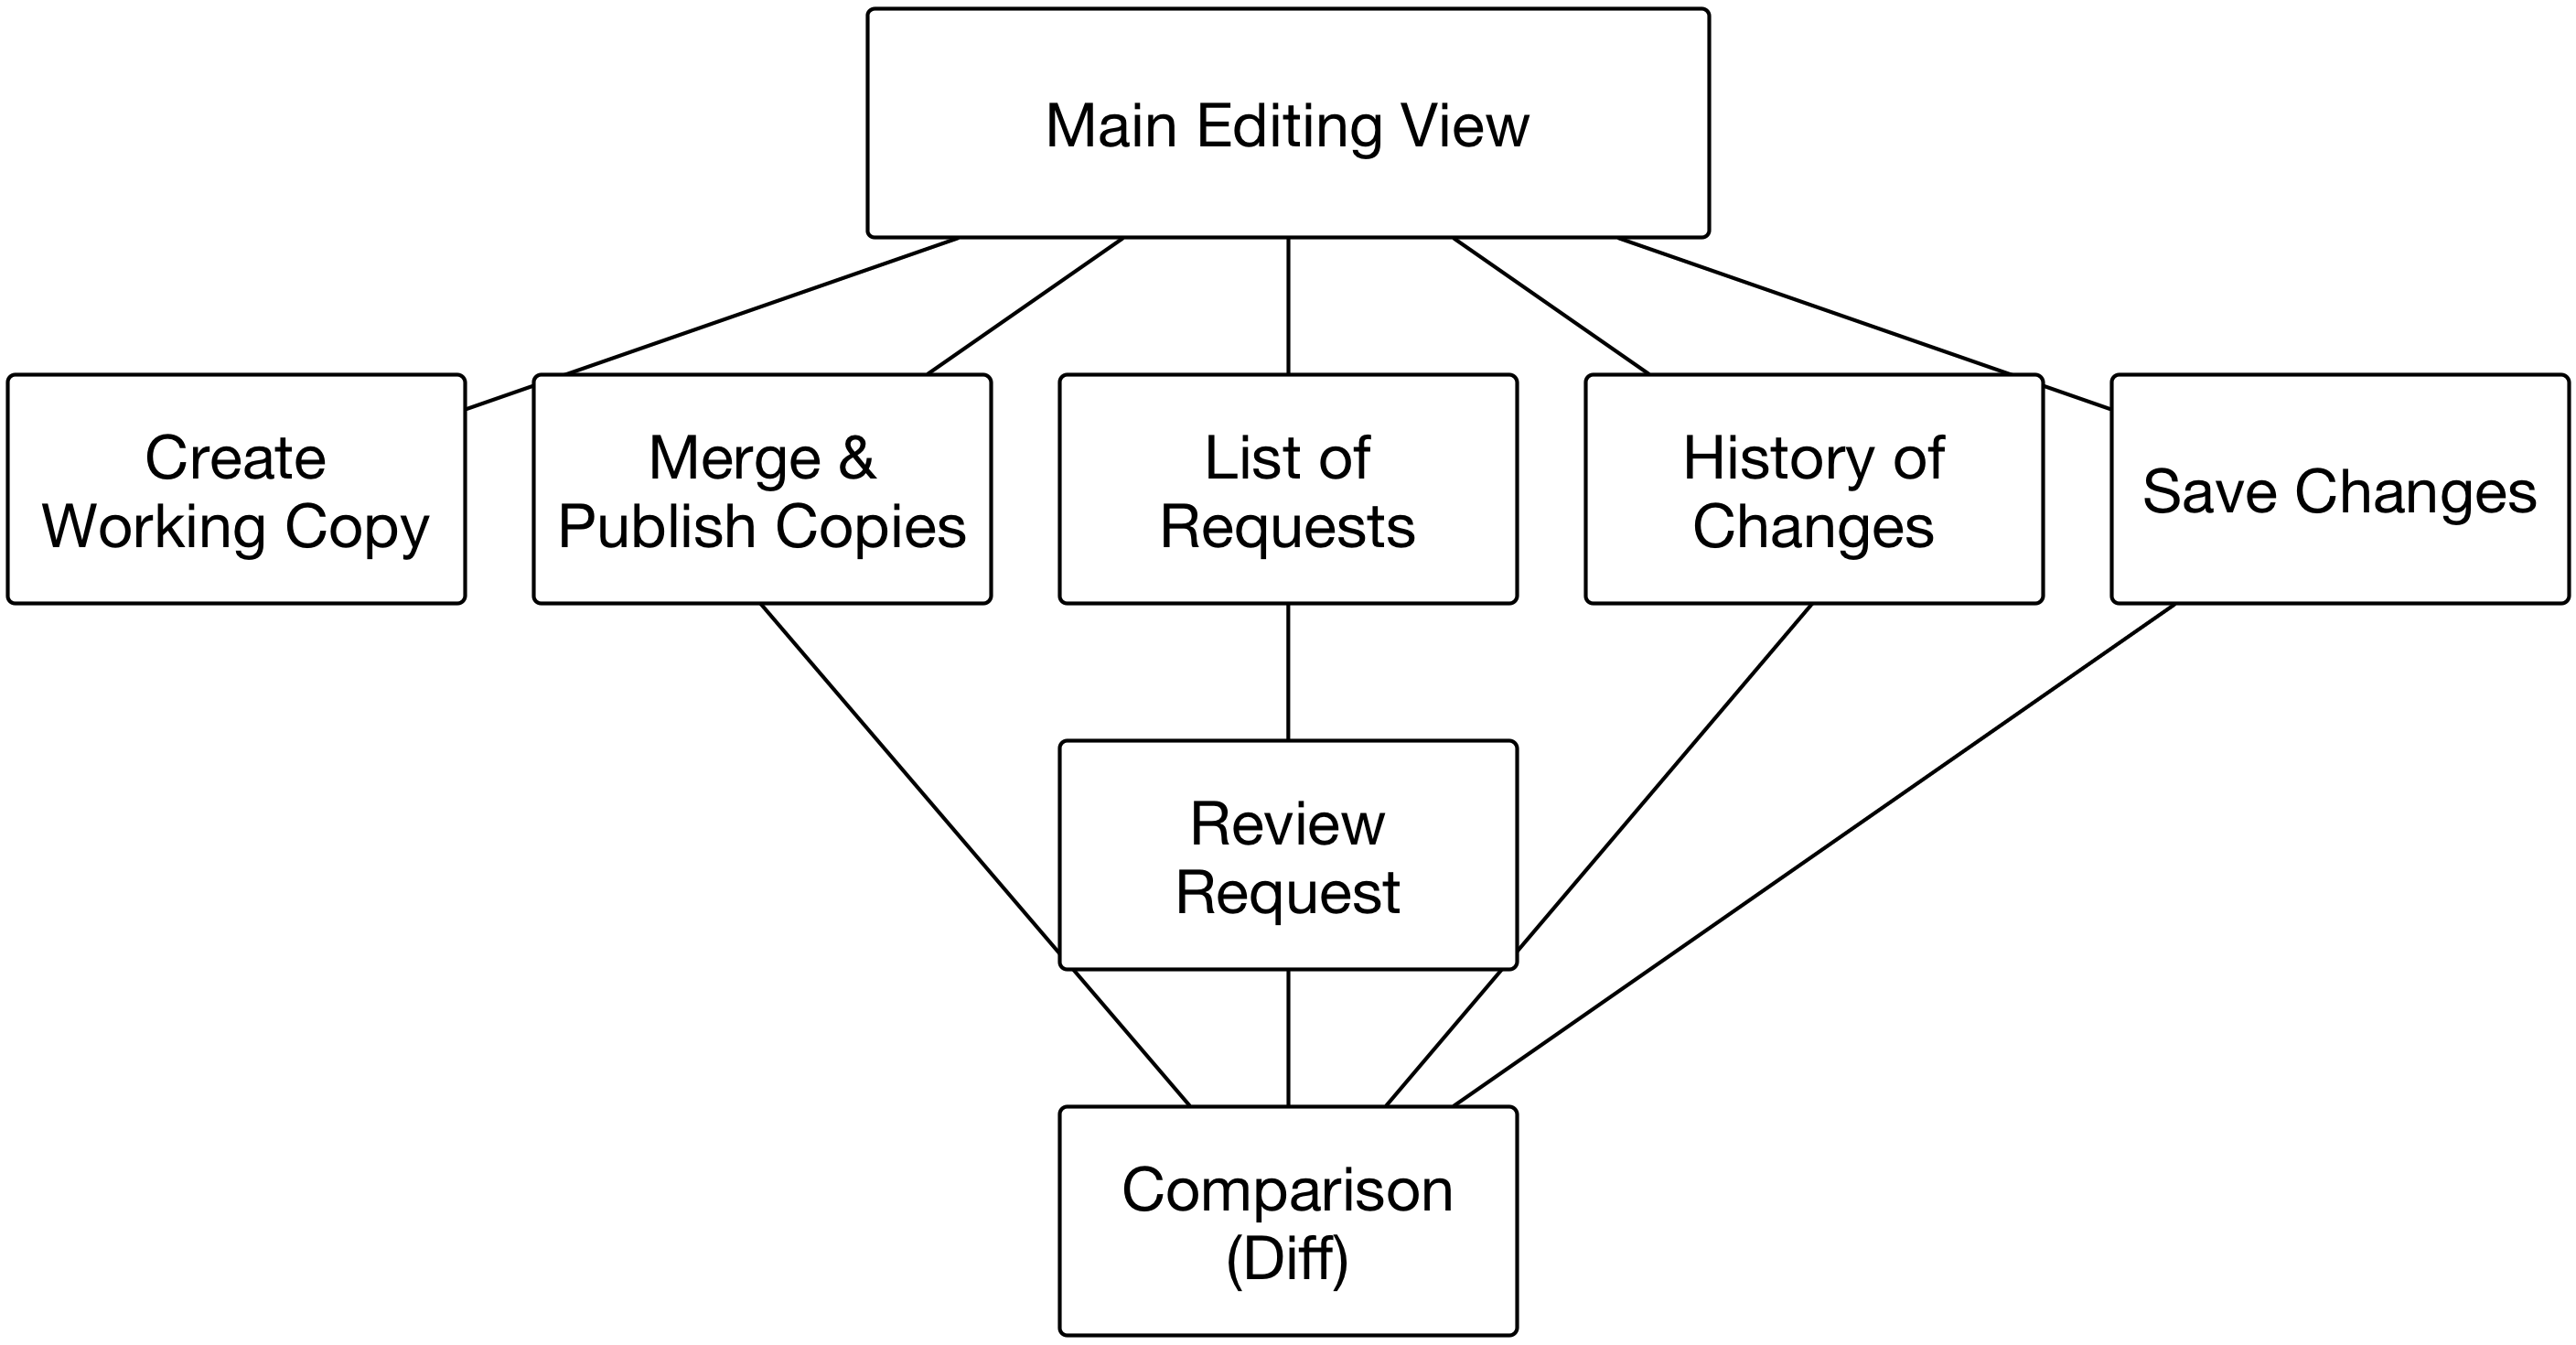
\includegraphics[width=11cm]{second-iteration/main-views-diagram}
 \caption{Main parts of the application}
 \label{fig:main-views-diagram}
\end{figure}

%In addition, Section \ref{sec:navigation-revised-terminology} highlights how the results of the focus group influenced the new terminology used within the interface.

%Additionally a lot of smaller changes were done as well, such as improving error messages, rephrasing explanations or reordering certain elements within views.

%As compared to the first prototype, the design was no longer just black and white, but utilized the Babbel corporate identity, so that it was closer to how a finished tool would look like. Additionally, the interface went from a semi-interactive prototype, based on graphical layouts, to a fully interactive web application. The prototype was based on AngularJS \cite{_angularjs_????}, a framework initially intended to facilitate rapid prototyping, which has evolved into a full-fledged frontend framework for developing single page web applications. These applications feel much more like Desktop-Applications than Websites, because new content is loaded asynchronously and therefore there is no visible interruption when navigating the app. The prototype was not fully functional, but covered the main version control features like its predecessor.

% \section{Usability Issues}
% Table \ref{sec:navigation-revised-terminology} shows the most problematic usability issues of each feature area discovered during the previous study. The table is sorted by the issue number and the following sections refer to these issues numbers to underline what problems have been solved by redesigning the different interface parts.

% \begin{table}[h!]
% \centering
% \begin{tabular}{|l|p{6cm}|l|l|l|}
% \hline
% \rowcolor[HTML]{EFEFEF}
% \textbf{\#} & \textbf{Usability issue} & \textbf{Feature area} & \textbf{Impact} \\ \hline
% 1 & Create new branch button was not found & Branches (Working Copies) & 40 \\ \hline
% 2 & Warning about editing content inside the master branch was ignored & Branches (Working Copies) & 40 \\ \hline
% 6 & Concept of a pull request is not clear (term might be confusing) & Pull Request & 40 \\ \hline
% 11 & New translations listed in the diff view are confusing, because the left column is empty (some users expected to see the learning language text) & Diff & 80 \\ \hline
% 12 & Not clear how to get from the diff view to the editing view & Diff & 40 \\ \hline
% 14 & Save button was not found (expected at bottom of screen) & Saving Process & 80 \\ \hline
% 19 & Visual representation/hierarchy of items/exercises not entirely clear & Main editing view & 18 \\ \hline
% 23 & Main navigation not completely obvious, clicking through (trial \& error) & Navigation & 20 \\ \hline
% \end{tabular}
% \caption{Usability issues with the highest impact scores from each feature area}
% \label{table:issues-most-impact-first-study}
% \end{table}

\section{Navigation and Terminology} \label{sec:navigation-revised-terminology}
During the first usability study as well as the subsequent focus group, the version control terminology has been identified as a major usability issue (Issues \#4, \#6 and \#23). Users especially struggled with grasping the concepts behind branches and pull requests. Based on the results and the input from the focus group, new names were conceived for some of the main features. Most notably, branches are now called working copies, or just copies, and pull requests are referred to as merge or publish requests. The term copy was chosen, because it is part of everyday language and much less abstract than the term branch. "Pull" was swapped for "merge" or "publish", because it describes the action of combining two different states of the content much better.

Additionally, the names of most features now signify an action (unsaved changes is now save changes, pull requests is now review requests, create pull request is now merge or publish). The intention behind this was to signal the result of an action to the user upfront and thus allow him or her to anticipate the result of an interaction.

Besides improving the used terminology, the design of the navigation bar was also slightly tweaked. Most importantly, all items now have labels and icons that visualize the feature, which could help users to orient themselves in a better way (Issues \#1 and \#25). Because this takes more space now, the repository (language package) selection has been moved to the upper right corner (Figure \ref{fig:nav-bar-old-new}).

\begin{figure}[h!]
 \centering
 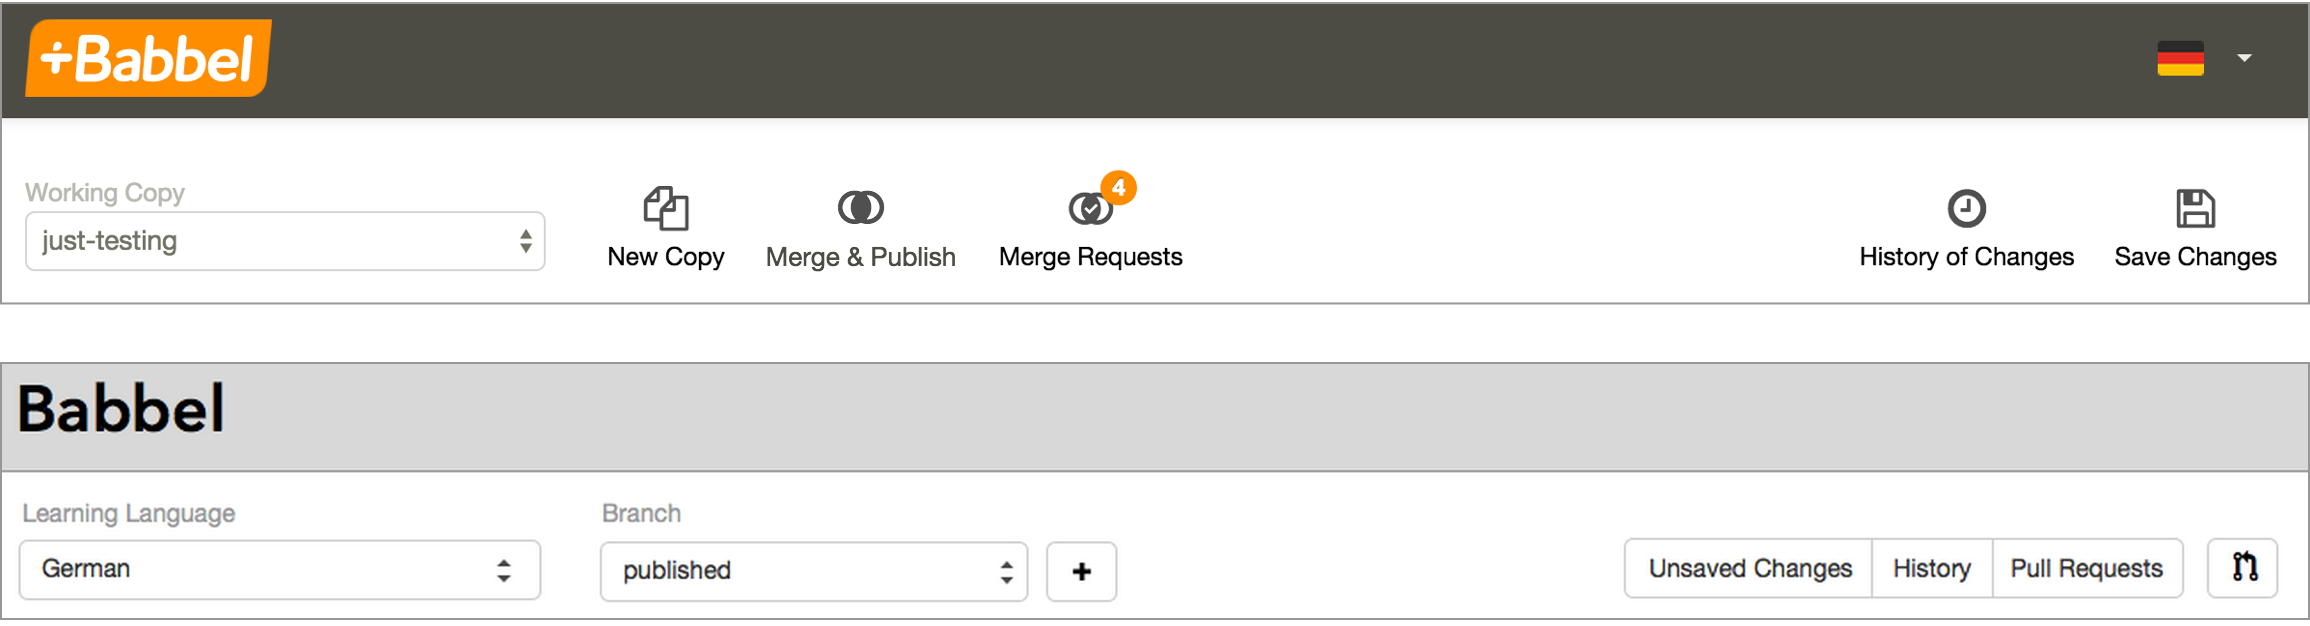
\includegraphics[width=\textwidth]{second-iteration/changes/nav-bar-old-new}
 \caption{New and old navigation bar}
 \label{fig:nav-bar-old-new}
\end{figure}

\section{Branches/Working Copies}
During the previous usability study the branch concept presented some serious problems to users. First of all, most participants were confused when being informed that editing the main branch is not possible (Issue \#2) and just ignored the message. Afterwards, many took some time till finding the functionality of creating a new branch (Issue \#1).

The warning message in the previous prototype (Figure \ref{fig:live-data-warning}) did not offer any solutions to the users. This lead to a situation where many users were lost after the message appeared. In order to mitigate this problem the new warning message now offers solutions right away. Users can choose to create a new working copy or dismiss the warning and edit the live content anyway.

Additionally the main branch was renamed from \emph{master} to \emph{published} to make it even clearer which kind of content is inside, thus fixing Issue \#3 and \#4.



%In most version control systems it is regarded as a best practice to make changes only on feature branches and thus keeping the main branch (master) always in a functional state. The same workflow is desired for content authoring since the public content should always be in an error-free state so that Babbel end-users always get the best possible experience. Not editing the live content directly thus reduces the risk of introducing new errors and allows collaborators to review changes before they are merged. For this reason, a warning message informs users when they are editing the main branch. This warning lead to some confusion during the first usability study. Users noticed they had

%In order to make the version control capabilities of the new content authoring tool as easy to use as possible the system offers a lot of explanations and assists users in making the right decisions. For example there is a warning when users are editing the live content/main branch (Figure \ref{fig:live-data-warning}).



\begin{figure}[h!]
 \centering
 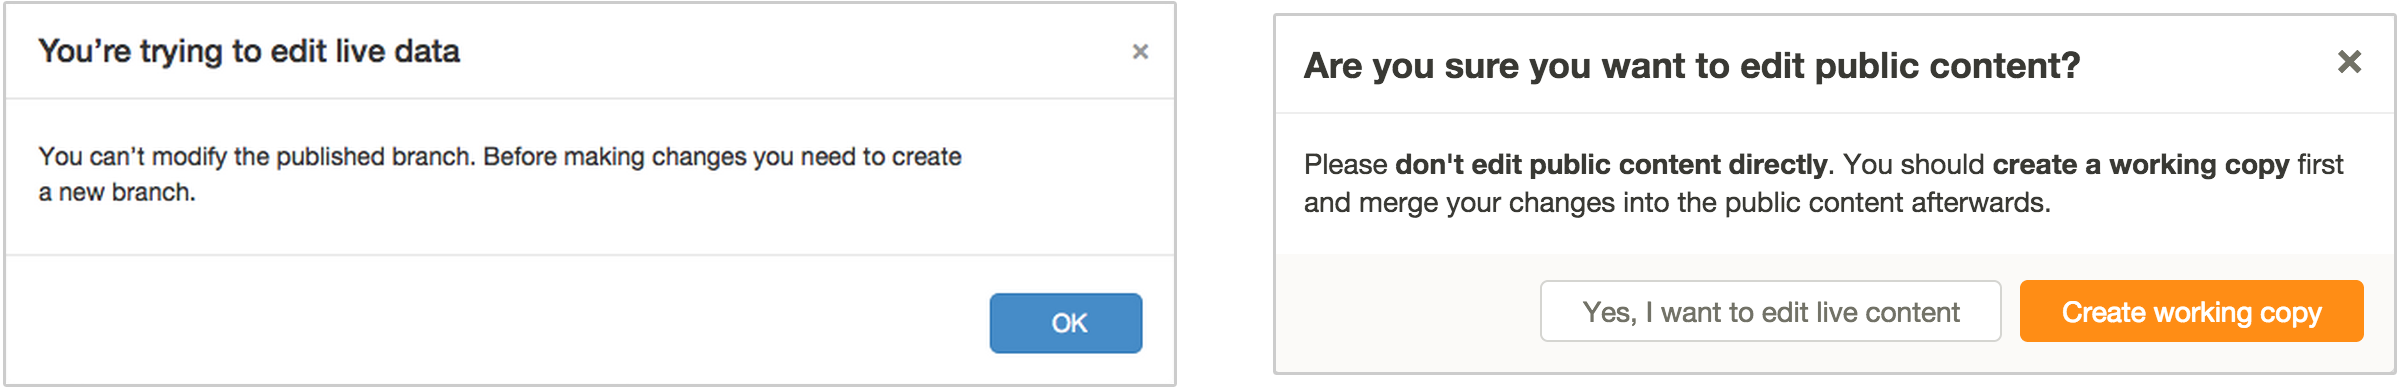
\includegraphics[width=\textwidth]{second-iteration/changes/live-data-warning}
 \caption{Live data warning old vs. new}
 \label{fig:live-data-warning}
\end{figure}

% \section{Issue \#6: Updated Terminology} \label{sec:changed-terminology}
% The focus group gathered after the first usability study made clear that the technical version control terminology used for the first prototype is only poorly understood. Therefore, new terms were conceived for the features least understood. In general, these were branches and pull requests.

\section{Improved Diff View}
The diff view posed some problems to users when looking at added translations (Issue \#11). Because the previous state was no translation at all the view showed a red empty box. Some users mistook this for a missing translation or an indication of an error, because of the red color (Issue \#13). The new design used a gray box instead to show that there was nothing before (Figure \ref{fig:improved-diff-view}).

Issue \#12, which prevented users from navigating from the diff view to the editing view, was addressed by underlining the breadcrumb, so that it became clearer that one can interact with it. Furthermore, instead of the button saying "show item" it was now labeled "edit lesson", which is hopefully clearer as well.

\begin{figure}[h!]
 \centering
 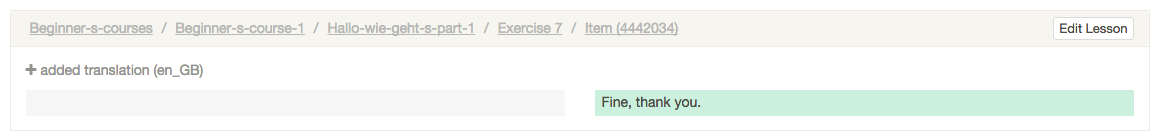
\includegraphics[width=\textwidth]{second-iteration/changes/improved-diff}
 \caption{Improved diff view}
 \label{fig:improved-diff-view}
\end{figure}

\section{Saving Process}
As Figure \ref{fig:saving-shortcut} shows the editor view now offers a shortcut for saving changes. In the design of the first iteration users were forced to use the save changes view (Figure \ref{fig:save-changes}), which also shows the differences between the old and the new state of the content. This is of course useful if a lot of changes have been done, especially across several lessons. But, the last study has shown, that users do not necessarily work that way (Issue \#18) and that it is often more convenient to save small changes right away. Therefore a simple save button at the bottom of the content table was introduced.

Furthermore, Issue \#16, which was related to the naming of the "back to editor" button and the fact that users confused its meaning with a "real" content editor, was solved by using a simple \emph{x} instead, which is often used for closing views or popups.

\begin{figure}[h!]
 \centering
 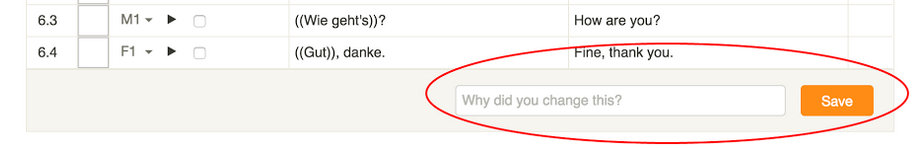
\includegraphics[width=\textwidth]{second-iteration/changes/saving-shortcut}
 \caption{Saving shortcut}
 \label{fig:saving-shortcut}
\end{figure}

\begin{figure}[hp!]
 \centering
 \fbox{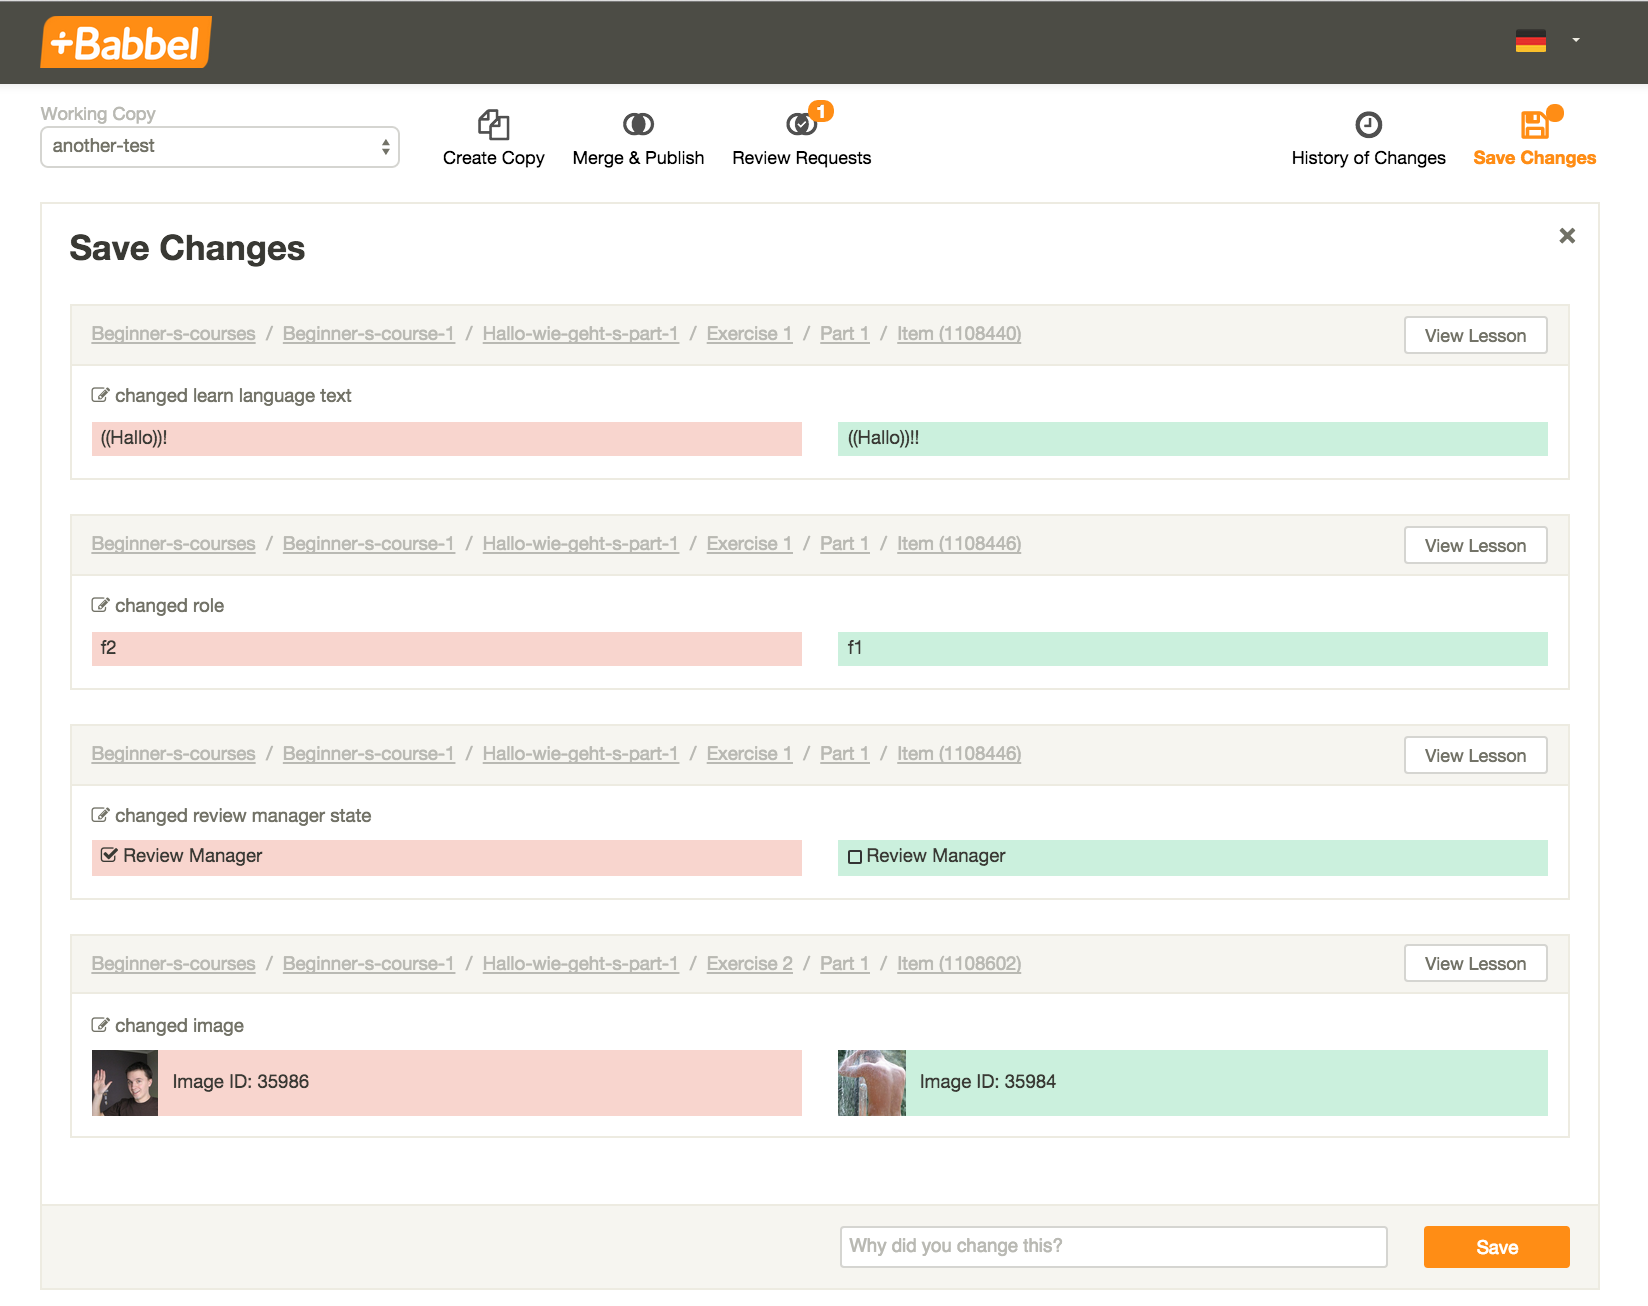
\includegraphics[width=\textwidth]{second-iteration/save-changes}}
 \caption{Save changes}
 \label{fig:save-changes}
\end{figure}

\section{New Content Representation}
For the new interface a different content representation was designed (Figure \ref{fig:main-editing-view}). The old one, which was using so called accordions, hid a lot of information in the beginning. According to the Yahoo Developer Network, the main reason for using accordions is "to compress a large amount of options into a limited space"\footnote{https://developer.yahoo.com/ypatterns/navigation/accordion.html}. This design pattern has the advantage to provide users with a quick overview, but the downside is that some information can only be exposed through a user interaction. Bret Victor explained this phenomenon as "harmful interaction" and provides the insight that good software design is often just good graphic design \cite{victor_magic_2006}. The accordions were one of the reasons why Scenario 3 presented such a hurdle for most users during the last study (Issues \#19 and \#20). Therefore, the new design uses a table layout which presents most of the important information at a glance. The intention is to provide a better overview without necessary interaction and thus enable users to find errors or problems in the overall lesson structure more quickly. Furthermore, this spreadsheet-like design should be very familiar to most users, since spreadsheets were used a lot as an auxiliary tool before, as described in Section \ref{sec:task1}.

% \section{Visualisations}
% Even though the visualisations were appreciated by the participants in the first user study, they were changed in the new interface. This is due to the fact that branches are now called copies and the old visualisations might have been confusing in conjunction with this slightly changed concept. Therefore the visualisations were swapped for simpler icons that indicate what is happening. Creating a new working copy is now visualised by two file symbols lying on top of each other (Figure \ref{fig:working-copy-creation}). The merging view now shows an icon similar to a Venn diagram, which indicates that only the differences between the first and the second copy will be merged into the second one.

% \begin{figure}[h!]
%  \centering
%  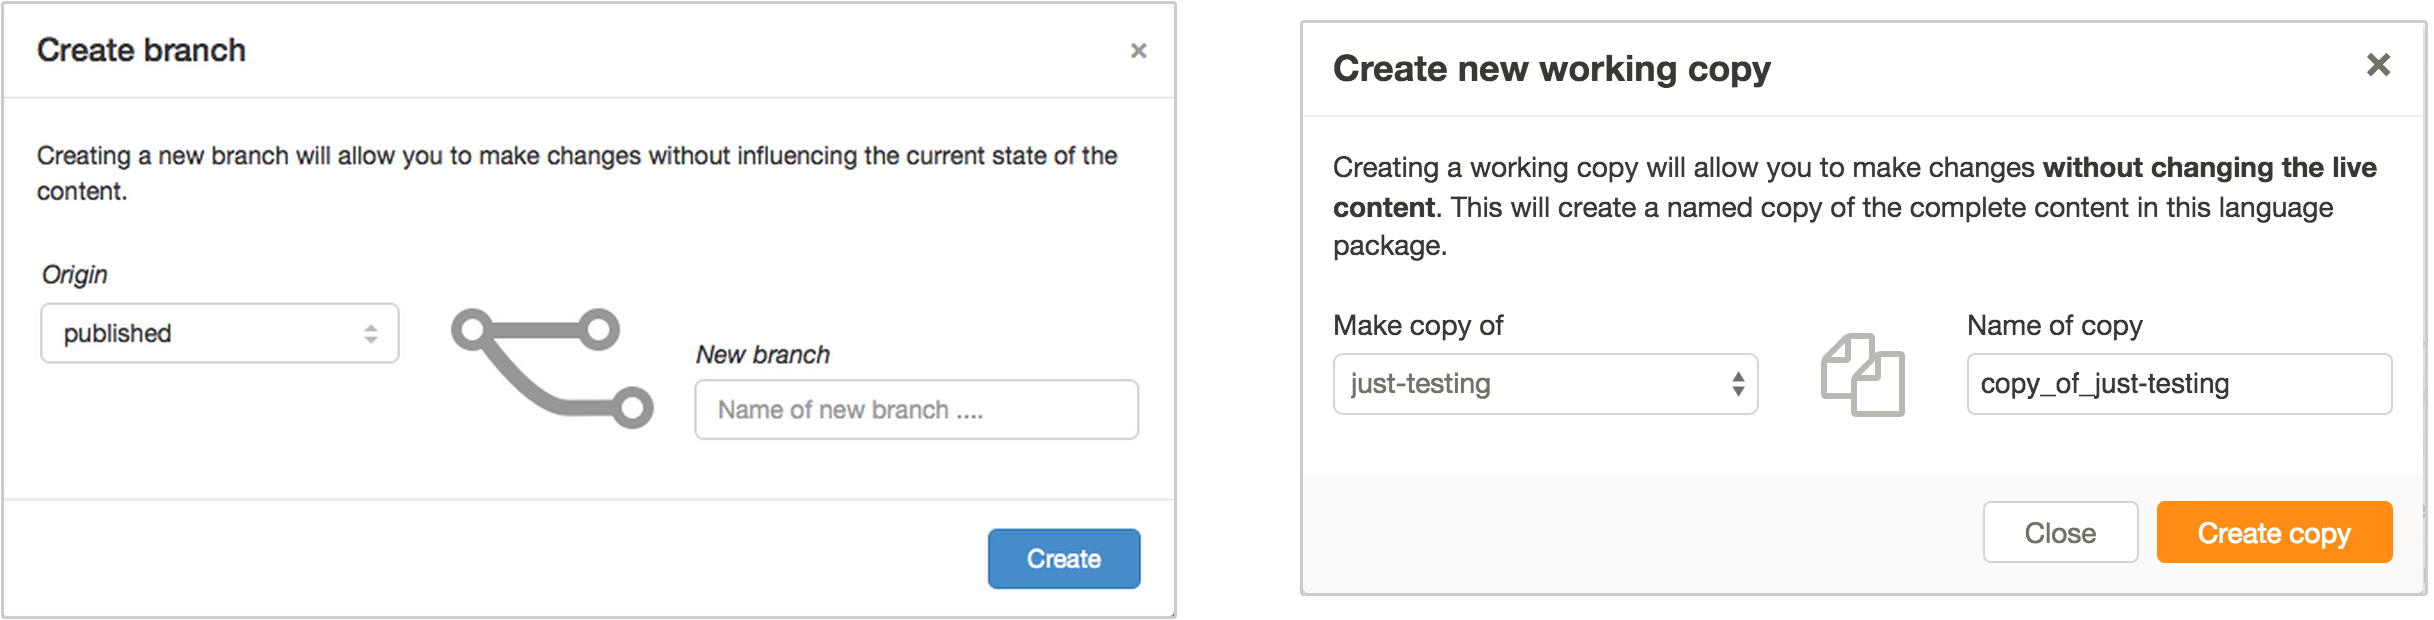
\includegraphics[width=\textwidth]{second-iteration/changes/working-copy-creation}
%  \caption{Creating branches/copies old vs. new}
%  \label{fig:working-copy-creation}
% \end{figure}

% \begin{figure}[h!]
%  \centering
%  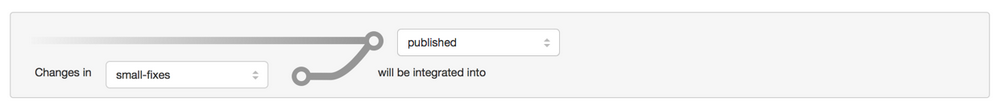
\includegraphics[width=\textwidth]{second-iteration/changes/merge-vis-old}
%  \caption{Merging branches old design}
%  \label{fig:merge-vis-old}
% \end{figure}

% \begin{figure}[h!]
%  \centering
%  
\includegraphics[width=\textwidth]{second-iteration/changes/merge-vis-new}
%  \caption{Merging copies new design}
%  \label{fig:merge-vis-new}
% \end{figure}


\begin{figure}[hp!]
 \centering
 \fbox{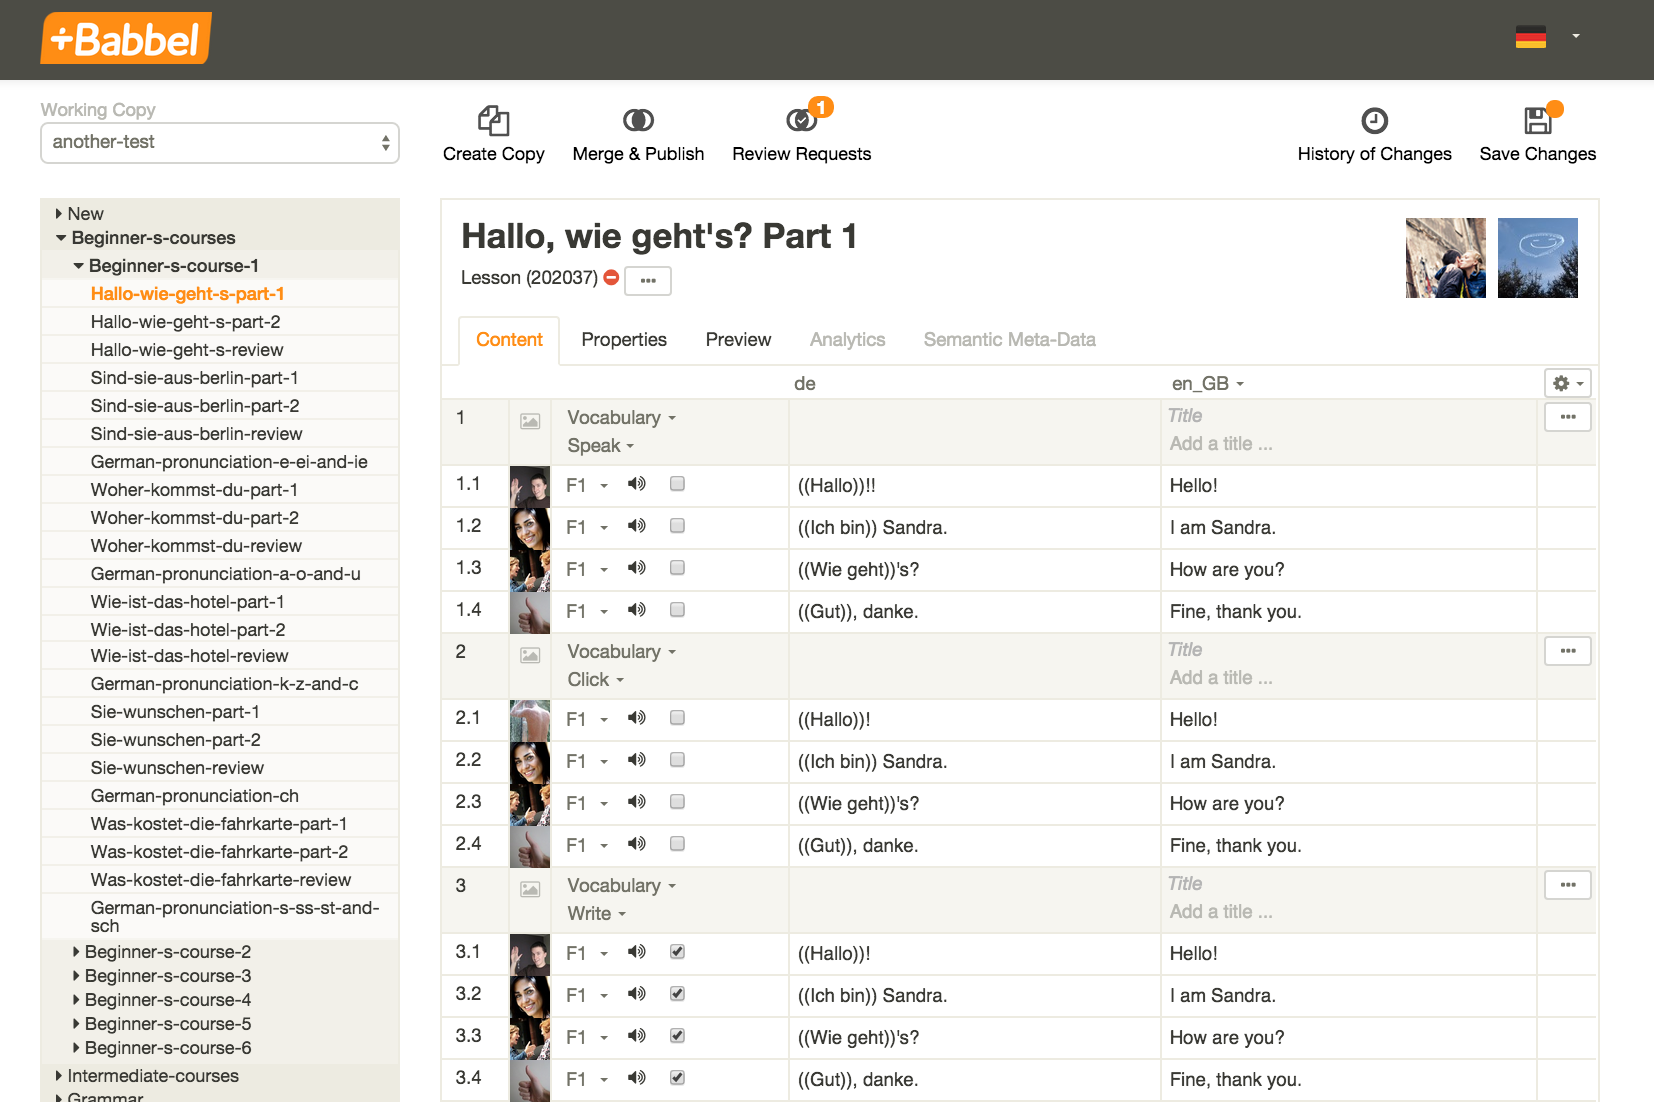
\includegraphics[width=\textwidth]{second-iteration/content-editing}}
 \caption{Main editing view}
 \label{fig:main-editing-view}
\end{figure}

\begin{figure}[hp!]
 \centering
 \fbox{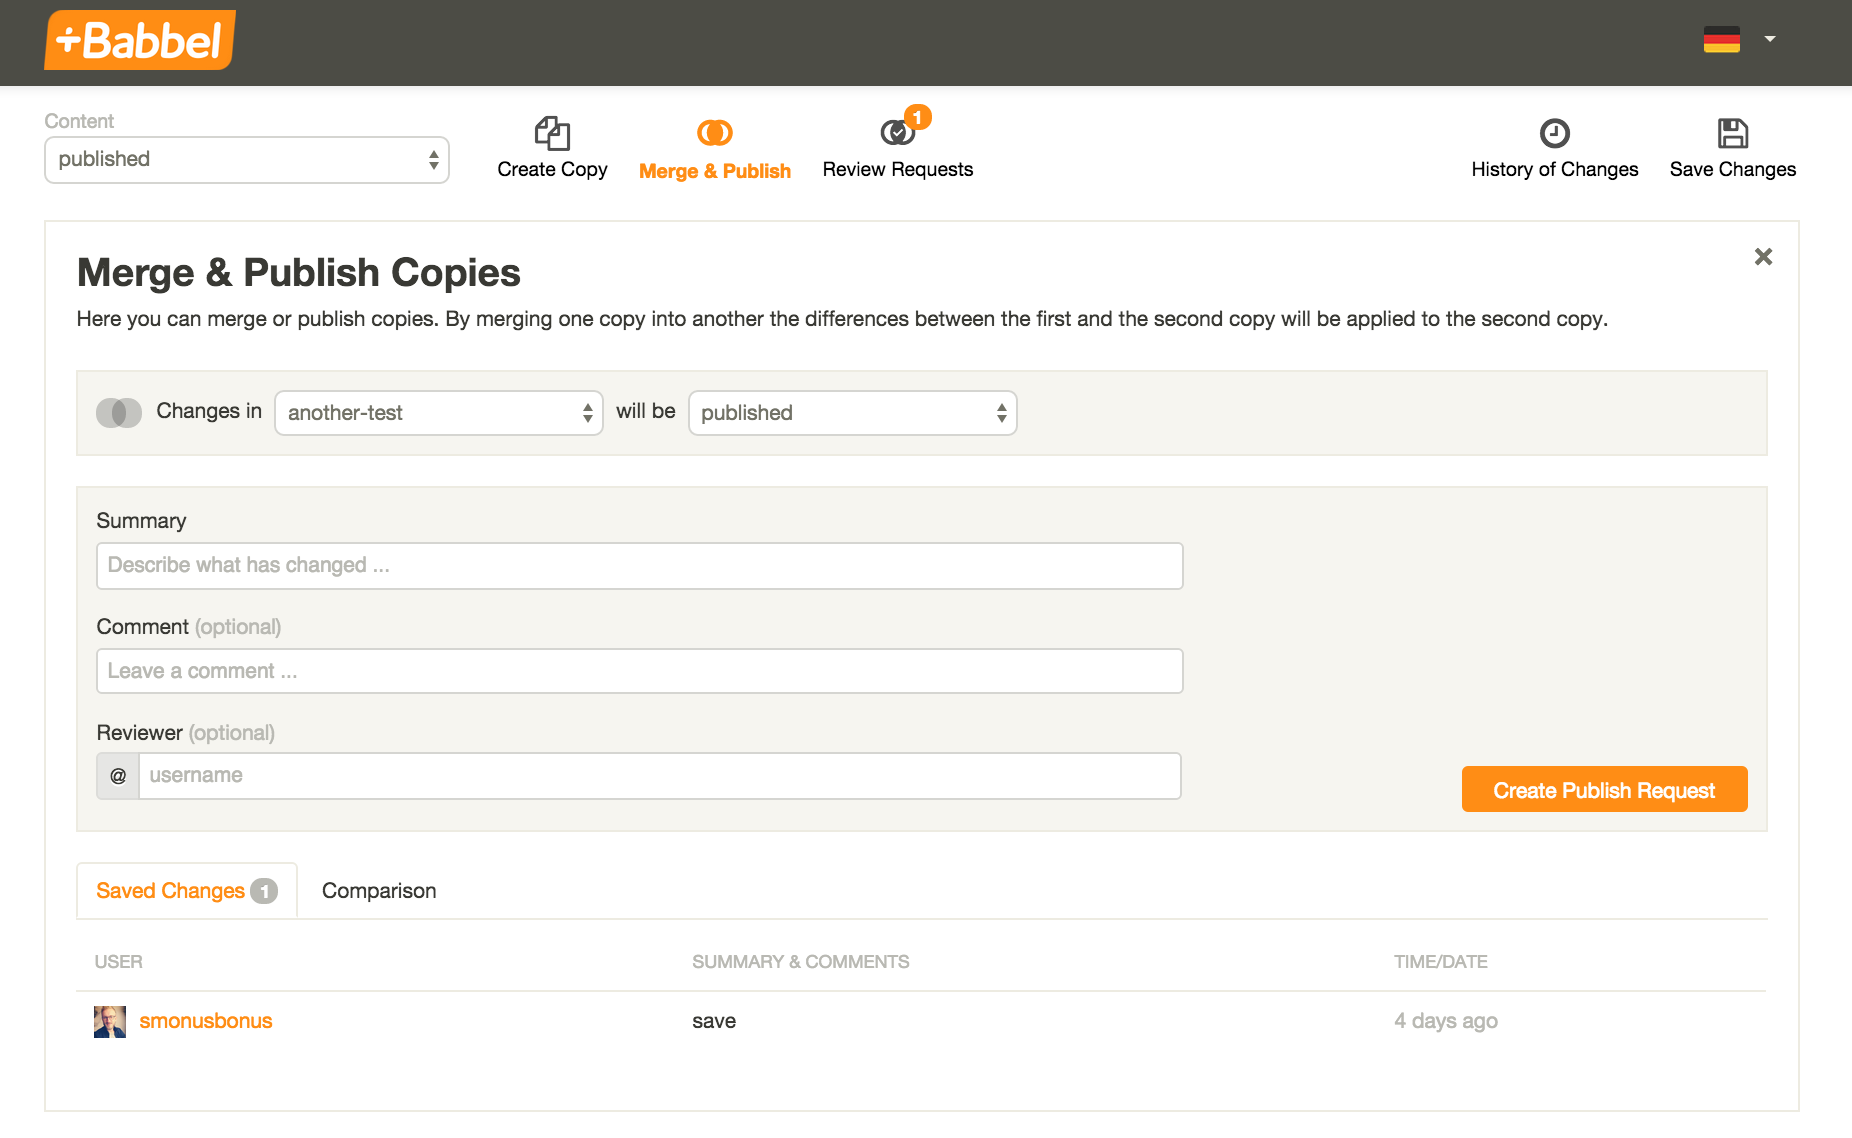
\includegraphics[width=\textwidth]{second-iteration/merge-copies}}
 \caption{Merge or publish copies}
\end{figure}

% \begin{figure}[hp!]
%  \centering
%  \fbox{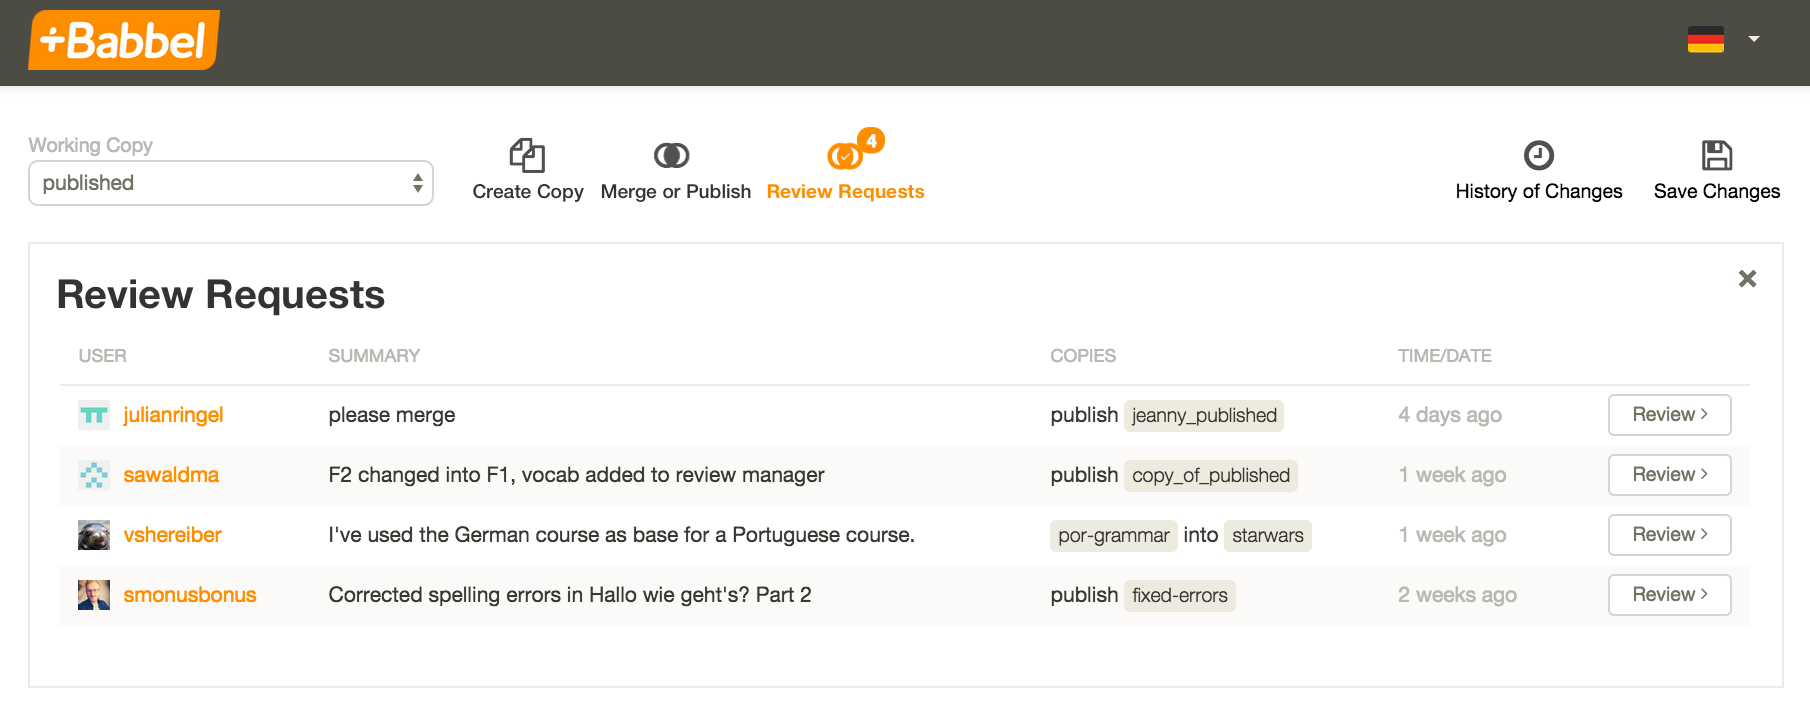
\includegraphics[width=\textwidth]{second-iteration/list-of-requests}}
%  \caption{List of requests}
% \end{figure}

\begin{figure}[hp!]
 \centering
 \fbox{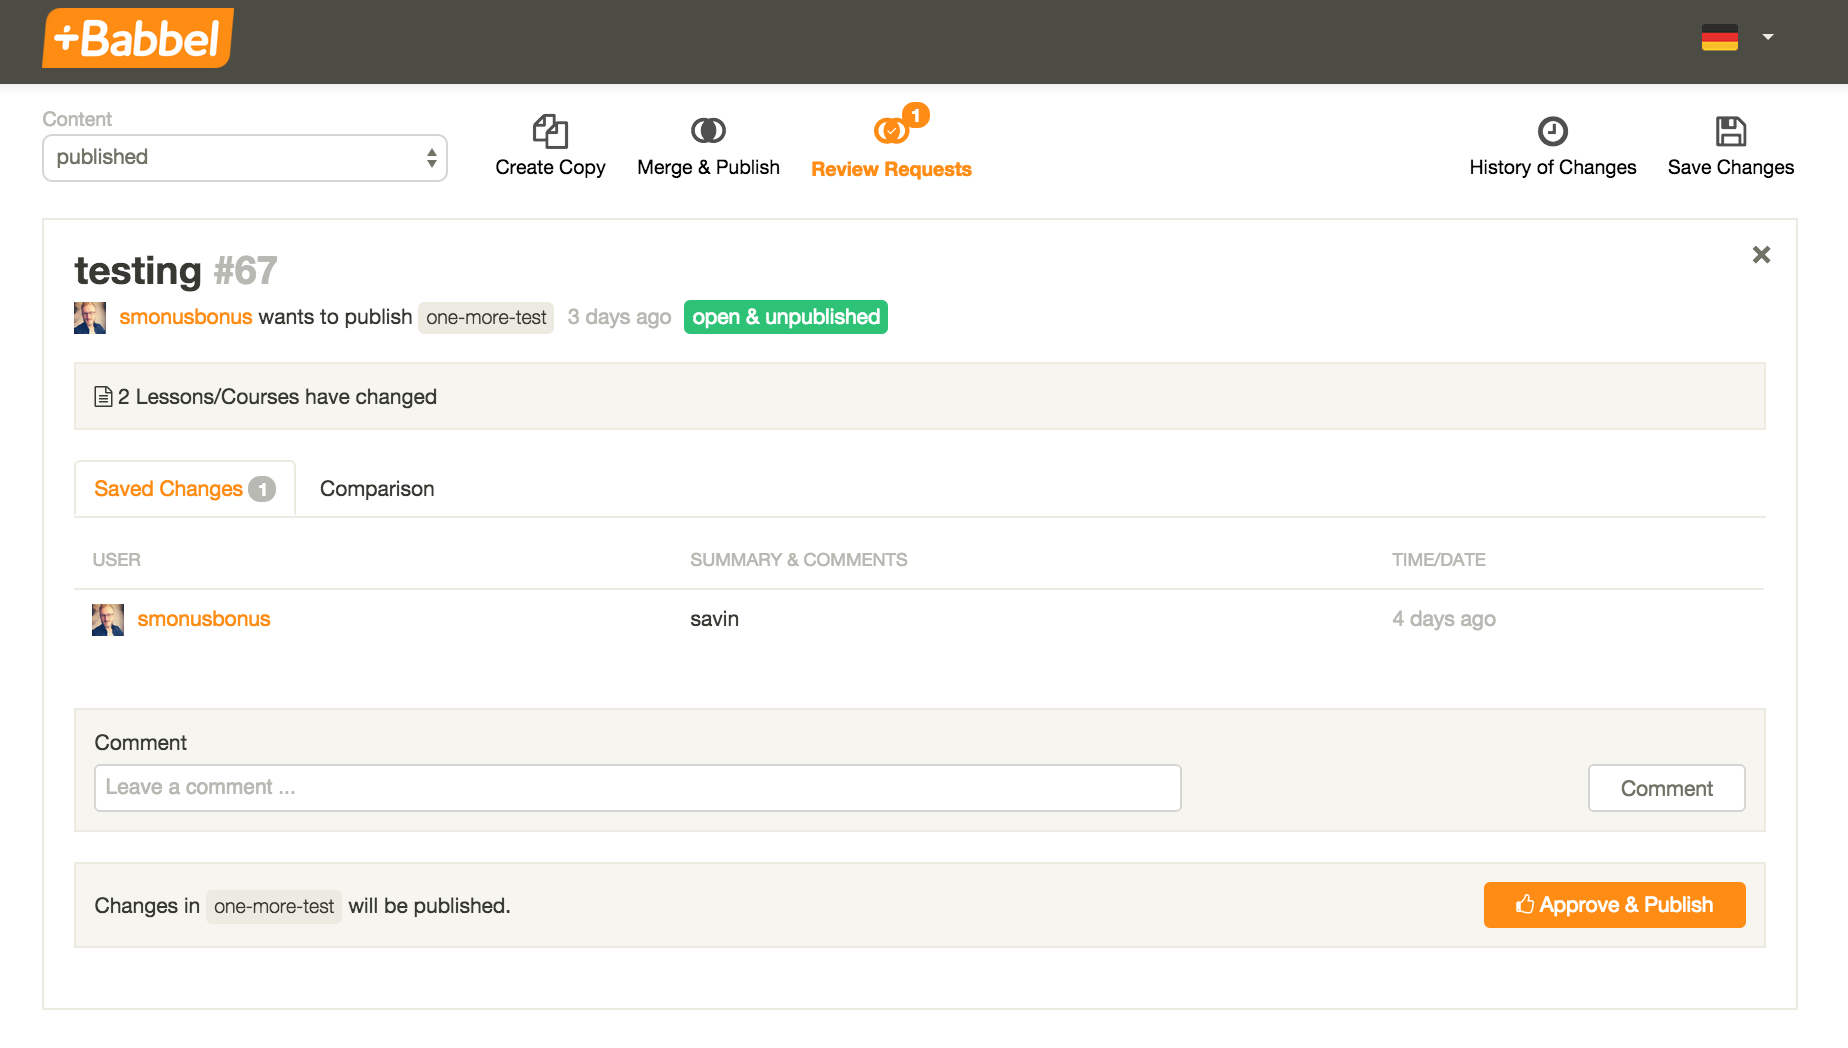
\includegraphics[width=\textwidth]{second-iteration/request-detail}}
 \caption{Review request}
\end{figure}

\chapter{Second Usability Study} \label{chapter:second-iteration}
The previous chapter described how the insights gained during the first study have been translated into redesigned interactions and new interface components. This chapter now looks at how, during the second usability study, the effects of these changes were measured.

\section{Study Design}
% general purpose of study
Whereas the first usability study was mostly about evaluating the high-level aspects of the interface and finding out which areas of the application caused the most serious problems, the second study was more about validating that the introduced changes had a positive impact on the user experience. Furthermore, the general suitability in regards to the envisioned purpose of the system was evaluated. In order to make the results of the first and second study comparable, the setup, especially in regards to the user scenarios, was kept similar.

% prototype - what was tested?
The screens shown in the previous chapter were part of a web-based prototype, that utilized a framework for rapid application development, called AngularJS \cite{_angularjs_????}. Whereas the prototype in the previous study still lacked a couple of important features, such as error messages, the system that was tested in this study was already functional to a large degree. This meant that users could freely interact with the system and therefore the sessions provided a fairly realistic picture of how the system would be used in a real-world environment later on.

% benchmark (metrics and questionnaire)
Additionally to verifying that the introduced changes had indeed improved the usability, a benchmark was established for the very first time. The benchmark was based on the metrics and the post-study questionnaire. Whereas the metrics answered the question whether a goal is reachable within a certain time-frame and by only committing a small number of errors, the questionnaire provided insights into how well the system was perceived in general and which feature areas still need improvement. The benchmark serves as a baseline for other researchers who want to draw on the ideas presented in this thesis and can also be used to evaluate future developments of the system at Babbel.

\subsection{Participants}
The participants of the second usability study were different from the ones during the first study. This was done to ensure that no learning effect would influence the results. Furthermore, it was important that users encountered the concept of version control for the first time when performing the tasks. All participants were selected randomly on a first come first serve basis. As can be seen in Table \ref{table:participants-study2} they represented a diverse group of people. Most of them were part of different language teams and also had different responsibilities within the content creation process. Most participants were content editors and one was a project manager.

As compared to the first study the number of participants was doubled. This was done in order to get more reliable results for the metrics and the newly introduced post-study questionnaire.

\begin{table}[h!]
\centering
\begin{tabular}{|l|l|l|l|}
\hline
\rowcolor[HTML]{EFEFEF}
{\bf Participant} & {\bf Language Team} & {\bf Job Position} \\ \hline
1 & French & Content Editor, QA \\ \hline
2 & Swedish & Content Editor \\ \hline
3 & German, Polish & Project Manager \\ \hline
4 & French & Content \& Image Editor \\ \hline
5 & Portuguese & Content Editor \\ \hline
6 & French & Project Manager \\ \hline
7 & English & Content Editor \\ \hline
8 & Russian & Content Editor \\ \hline
9 & Russian & Content Editor \\ \hline
10 & German & Content Editor \\ \hline
\end{tabular}
\caption{List of Participants}
\label{table:participants-study2}
\end{table}


\subsection{Metrics}
The same quantitative metrics as during the first study were collected. Comparing those might provide helpful insights into what has improved or not.

\begin{itemize}
 \item{\emph{Successful Task Completion}: percentage of tasks that were completed successfully}
 \item{\emph{Time On Task}: time that was needed to perform a task}
 \item{\emph{Error Rate}: participant deviated from “ideal” path of navigation, such as opening the wrong menu.}
 \item{\emph{Scenario Specific Metrics}: such as how long it takes to find the missing translation in Scenario 3 or how quick users discover the create copy function}
\end{itemize}

\subsection{Scenarios}
Scenarios 1 to 3 were identical to the ones used in the first study (as described in Section \ref{sec:scenario-descriptions}). The fourth task has been added to the study in order to lay more focus on the new content representation (main editing view).

The procedure, especially in regards to the scenarios, was kept more or less consistent in order to make comparing the results of the two studies simpler. The interface could be regarded as the independent variable. This means that new results are not influenced by a changed session procedure, but instead can be mostly attributed to the changes in the interface. Of course, given the small number of participants, the different abilities and professional backgrounds of the participants can affect the results as well.

\subsubsection{Scenario 4: Create Exercise and Fill With Content} Add a new memory exercise to this lesson (Link provided). Please don’t edit live content. The title of the exercise should be “awesome memory”. The translation visibility “partial”. Add 3 items to the exercise. Assign random images to the items. Assign all items the speaker role F1. Add all items to the review manager. Finally save your changes.

\subsection{Post-Study Questionnaire}
As an additional means of gathering feedback users were asked to answer a post-study questionnaire. A standardized questionnaire called PSSUQ (Post-study System Usability Questionnaire) was used. It consists of 16 questions that produce 4 different scores, which signify how well the system was perceived (Overall, System Quality, Information Quality, Interface Quality). The goal of utilizing this questionnaire was to reveal potential weak spots of the interface that were not discovered by observing participants. Note that the third version of the questionnaire was used, as recommended by Sauro and Lewis \cite{sauro_quantifying_2012}.

\subsection{Sessions}
Each session was scheduled for one hour. In the beginning participants were introduced to the procedure and the purpose of the study. Afterwards they had to fill in a short questionnaire which asked about their experience with version control systems and the current content authoring tool.

The largest part, going through the scenarios and performing the described tasks, was scheduled to take about 30 minutes. Some users took longer than that, but most finished within the expected time-frame.

Lastly, an open discussion was initiated were questions that arose during the scenarios could be answered and users could provide some general feedback. Usually they were asked about their general impression of the interface and what they liked and disliked most about it. The session concluded with the aforementioned PSSUQ.

\section{Findings}
The following section describes the most important findings of the second usability study. Where meaningful the findings are compared to those of the first study. These include quantitative metrics as well as the discovered usability problems.

\subsection{Metrics}
As during the first study quantitative metrics were recorded. Task completion rate, time on tasks and error rate. Furthermore, a few task-specific metrics were measured. For example for Task 1 it was measured how much time users needed to find the create copy/branch feature. This allowed for a more meaningful comparison as is described in the section below. For task 3 the time for finding the missing translation was recorded.

The tables below show a comparison between the metrics recorded during the first user study and the second. It should be noted that the studies carried out are focused on qualitative findings, which are mostly based on observations and discussions. The metrics only extend and support these findings, but they do not stand for themselves. Because of the relative small sample sizes and partially large variances this data should not be overrated.

\subsubsection{Task Completion Rate}
The task completion rates did not change that much except for Task 1 for which it increased 11 percentage points. One possible explanation is the newly designed warning message, that now offers a direct solution instead of just informing users (explained in more detail in the scenarios section below). Unfortunately, 61\% is still an unsatisfactory completion rate. Exactly why it is still so low is hard to tell. One reason for the low completion rate, especially in comparison with the other tasks, might be that users had to get used to the interface at first. The task order was not randomized but always remained the same. A randomized task order might have resulted in a more balanced rate, in particular between Task 1 and 3, which according to the participants were the most difficult tasks (4.8 and 2.7 on a scale from 1-7 where 1 equals very difficult).

\begin{table}[h!]
\centering
\begin{tabular}{|l|l|l|l|}
\hline
\rowcolor[HTML]{EFEFEF}
{\bf Scenarios} & {\bf First Study} & {\bf Second Study} & {\bf Difference in pp} \\ \hline
Scenario 1 & 50\% & 61\% & +11 pp \\ \hline
Scenario 2 & 100\% & 94\% & -6 pp \\ \hline
Scenario 3 & 70\% & 72\% & +2 pp \\ \hline
Scenario 4 &  & 100\% &  \\ \hline
\end{tabular}
\caption{Comparison of task completion rates during first and second user study}
\label{table:task-compl}
\end{table}

\subsubsection{Time on Tasks}
As Table \ref{table:time-tasks} shows the biggest difference is again observed for Task 1. Participants during the second study needed about 75 seconds less for finishing this task as participants in study 1. The scenario-specific metric provides an explanation for this. As can be seen in Figure 1, participants of the second study needed much less time to locate the create branch/copy feature then participants in study 1 who almost spent half of the time searching for this feature.

\begin{table}[h!]
\centering
\resizebox{\textwidth}{!}{%
\begin{tabular}{|l|l|l|l|}
\hline
\rowcolor[HTML]{EFEFEF}
{\bf Scenarios} & {\bf First Study (mean)} & {\bf Second Study (mean)} & {\bf Difference} \\ \hline
Scenario 1 & 367 & 292.25 & -74.75 \\ \hline
Scenario 2 & 128 & 146.57 & 18.57 \\ \hline
Scenario 3 & 395.5 & 369.42 & -26.08 \\ \hline
Scenario 4 &  & 280 &  \\ \hline
\end{tabular}
}
\caption{Time on tasks (in seconds)}
\label{table:time-tasks}
\end{table}

\subsubsection{Errors}
Even though the other metrics show most improvements for Task 1 this is not the case for the error rate. Here, there is only a slight decrease of errors for Task 1, whereas errors during the other tasks (2 and 3) have halved. A possible explanation for this might be the changed terminology, which allowed users to better orient themselves (action verbs and more everyday language than technical terms). It seems there was less trial and error when finding the right feature. The observations support this assumption; there were less users asking things like “What is a pull request?”.

\begin{table}[h!]
\centering
\begin{tabular}{|l|l|l|l|}
\hline
\rowcolor[HTML]{EFEFEF}
{\bf Scenarios} & {\bf Study 1} & {\bf Study 2} & {\bf Difference in Errors} \\ \hline
Scenario 1 & 2.2 & 1.87 & -0.33 \\ \hline
Scenario 2 & 1.6 & 0.5 & -1.1 \\ \hline
Scenario 3 & 4.2 & 2.12 & -2.08 \\ \hline
Scenario 4 &  & 0.5 &  \\ \hline
\end{tabular}
\caption{Comparison of error rates during first and second user study }
\label{table:second-study-error-rate}
\end{table}

\subsection{Impact of Design Changes}
The major changes implemented for this study had different levels of impact. Some of the changes were quite noticeable during the sessions whereas others are harder to validate.

\subsubsection{Navigation Bar \& Changed Terminology}
The new navigation bar did not attract a lot of attention, which is probably a positive sign. The reduced error rate could at least be partially attributed to the improved naming and the icons (Table \ref{table:second-study-error-rate}). In general, there seemed to be less trial and error when users navigated the application. During the previous study remarks like "What is a pull request?" and "I'm just going to click through, I have no idea" suggested that there is a usability problem. This time, these remarks were much less frequent. Especially the new terms "working copy" and "merge request" seemed to be much better understood than their predecessors. Furthermore, using action verbs to highlight what a feature can do instead of passively describing it cleared things up as well.

% \subsubsection{Visualisations}
% The new visualisations did not result in a noticeable change. Since the new terminology was more straightforward the need for visualisations could have been reduced by that as well (Figure \ref{fig:approve-request}).

% \begin{figure}[h!]
%  \centering
%  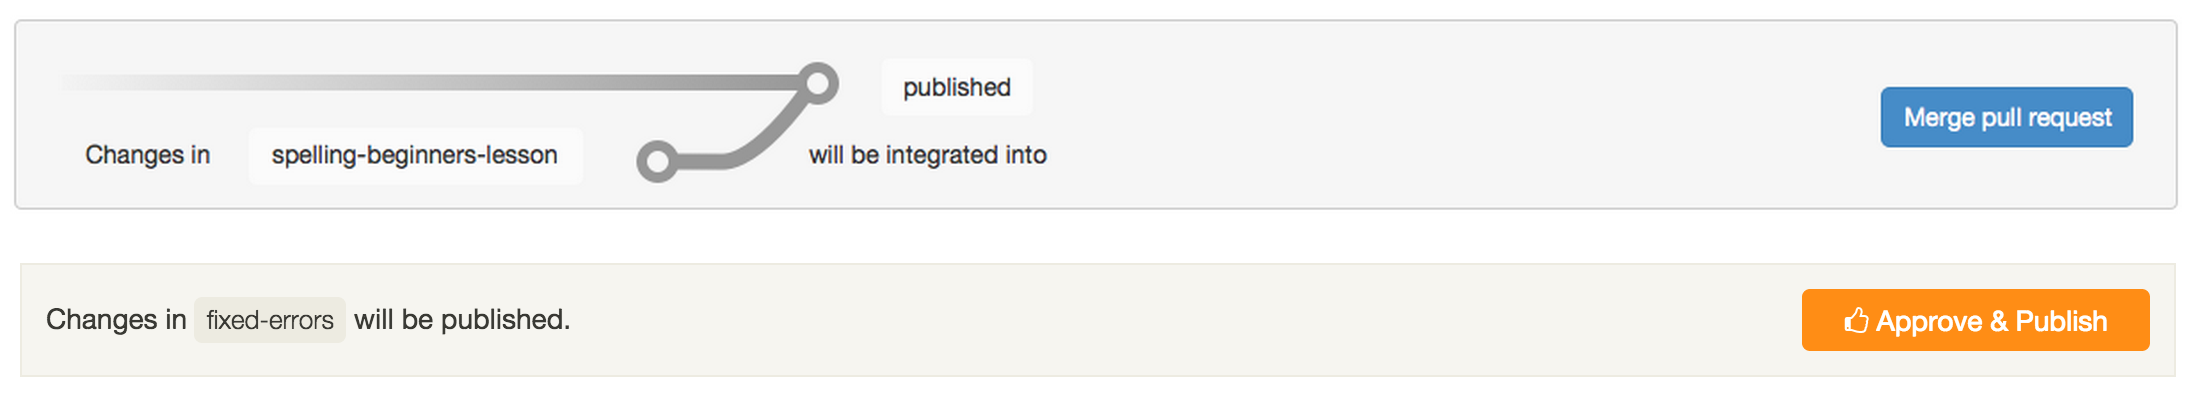
\includegraphics[width=\textwidth]{second-iteration/changes/approve-request}
%  \caption{Approving a request old vs. new}
%  \label{fig:approve-request}
% \end{figure}

\subsubsection{Saving Process}
A positive outcome of the newly added saving shortcut was that it was used a lot. The downside on the other hand was that some users got confused by the existence of two different saving features. The shortcut save sped up editing and users did not seem to miss the list of changes they would got with the "advanced" saving feature. What has become apparent is that the old saving feature, which concept-wise, is very much inspired by the staging area of version control systems, might not be the most intuitive solution for content editors. In programming there is often a need of touching many files at once to implement a new feature. In content editing this is seldom the case. Changes are usually logically tied to a single lesson.

\subsubsection{Live Content Warning}
Task 1 asked users to apply two small changes inside a lesson. The difficulty was that they were not supposed to edit the live content. That meant that they had to create a copy (branch) of the content first, make the changes, save them and finally merge the copy with the public content again. During the first study participants wasted a lot of time finding the create branch/copy feature after they had been alerted to not edit the live content. As Figure \ref{fig:avg-time-task1} shows this time could be greatly reduced through the new design in the second study. The dark grey bars show the moment in time when users discovered the feature. During the first study users spent almost half of the time with finding this feature whereas during the second study they discovered it a lot earlier. This also had an effect on the average time taken for Task 1 in total and the completion rate. These improvements are probably due to the redesign of the warning message as described in the previous chapter (Figure \ref{fig:live-data-warning}).

\begin{figure}[h!]
 \centering
 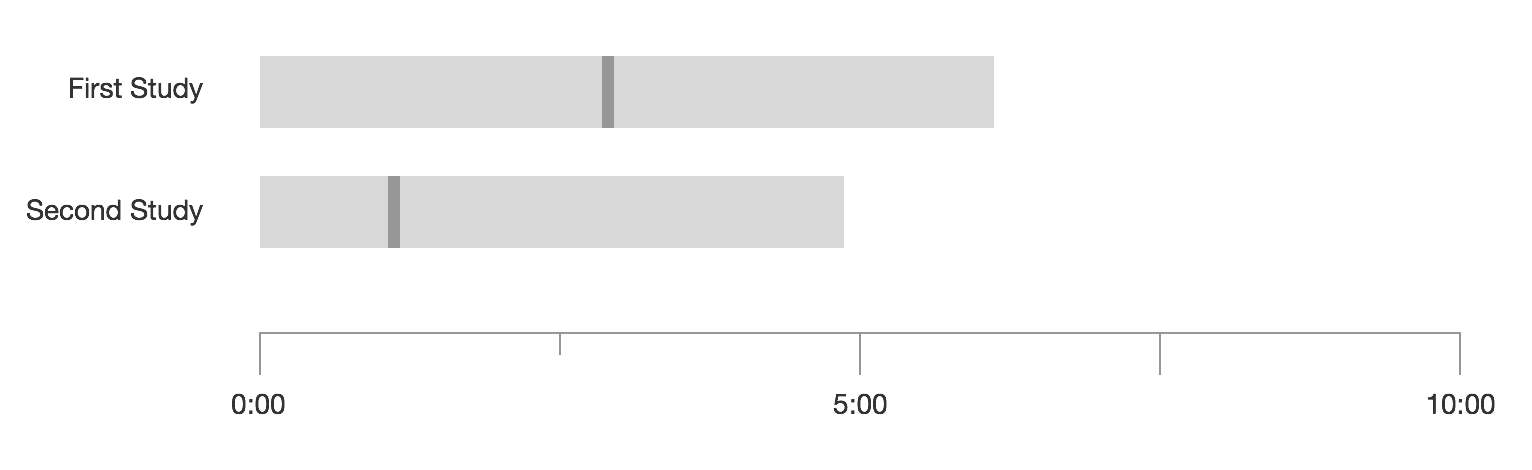
\includegraphics[width=12cm]{second-iteration/plot-branch-creation}
 \caption{Average task completion time and time of branch/copy creation}
 \label{fig:avg-time-task1}
\end{figure}

\subsubsection{Content Representation}
In general the new content representation performed quite well. This became apparent in Task 3 when users had to find a missing translation. Whereas, during the previous study, some users had problems locating this missing field within the content representation (because it was initially hidden), this was no longer a problem with the new design. Once users had arrived at the content of a lesson and selected the right language they could locate the missing translation quite quickly. The only noteworthy issues of the new design were malfunctioning popovers (did not close automatically) and labels that looked placeholders and were therefore selected by some users (instead of the actual input field).

%figure here of old new content representation (finding translation)


%\subsection{Scenario 2}
%Scenario 2, as during the first round of user tests, seemed to be the easiest one. 94\% completed the task with only 0.5 errors on average. This shows that the two main views needed for solving this task have a low number of usability issues. The reduced number of errors could also be attributed to the new naming. Instead of “Pull Requests” the feature was called “Review Requests” and instead of “Merge Pull Request” the command for merging changes was now called “Approve \& Publish” (Figure \ref{fig:approve-request}).

%\subsection{Scenario 3}
%Scenario 3 seemed again to be the most tricky one. Users especially struggled with finding the missing translation. Even though the new content representation made it easier to find the missing translation once they had navigated to the right lesson, most of them still got stuck in the list of changes and tried finding the missing translation there. Only 2 out of 10 users noticed that a translation that was forgotten could not show up in a list of changes, because it was never altered. The quotes below illustrate how users felt during this scenario.

%\subsection{Scenario 4}
%The observations of scenario 4 cannot be compared to the first study since it was introduced only for this study. The purpose was to assess the usability of the changed content representation and the ease of adding new content. This task, as task 2, posed relatively few problems to users. The only noteworthy issues are that popovers did not close automatically when clicked outside and labels that were confused with placeholders and therefore selected by some users (instead of the actual input field).


\subsection{Discovered Usability Issues}
Even though several usability issues were fixed as compared to the first study, there were also a lot of new ones coming up. Some of this might be due to the fact that users could now freely interact with the tool and were not constrained by the prototype design as in the first study. In total, the number of rather severe issues (Severity score of 10 or 5)  was reduced from 15 in the previous study to 11 during the second study. Also the impact of most issues was lower this time, which can be attributed to less users experiencing the problem.

The following section lists the usability issues discovered during the test sessions. As for the first study, the impact score by Sauro and Lewis \cite{sauro_quantifying_2012} was calculated for each issue and the tables are sorted by the highest impact scores. Please note, in order to avoid confusion later on, the issue numbers are continuous and thus start with 27.

% this is now described in the first study
% The following section describes the usability problems that have been discovered by observing participants performing the different scenarios. They are grouped by feature areas of the application and the most important issues are shortly explained. In order to rank the issues by their impact on the user experience a severity score was used, as suggested by Sauro and Lewis \cite{sauro_quantifying_2012}. The most severe issues, which prevented users from completing the tasks, were given a score of 10. 5 points were assigned if the issue caused a significant delay or frustration. 3 points were allocated for minor issues and just 1 point for improvements suggested by participants. To create an impact score the severity was multiplied by the frequency of users who experienced the problem (severity * frequency / 10). A frequency of 40\% means that 4 of 10 users encountered the problem, independent of whether they ran into the issue more than once. The scale ranges from 100 (most severe problem, experienced by all users) to 1 (suggestion by a single user).

\subsubsection{Working Copies}
Working copies, which were previously called branches, were in general quite well understood. Nevertheless, they also caused some usability issues. A common misconception was that a working copy only consists of one lesson, where in reality it contains the whole language package (repository).
Furthermore, the interface did not provide appropriate feedback when errors occurred, the feedback was either too general or completely non-existent (Table \ref{table:issues-copies}). Additionally, some users did not realize that after creating a new copy it was already selected. The name in the dropdown changed, but it is barely noticeable if you do not know where to look.

% \begin{displayquote}
% "I like that I get all this information." \textit{Participant 8}
% \end{displayquote}

\begin{table}[h!]
\centering
\begin{tabular}{|r|p{7cm}|r|r|r|}
\hline
\rowcolor[HTML]{EFEFEF}
{\bf \#} & {\bf Usability issue} & {\bf Severity} & {\bf Frequency} & {\bf Impact} \\ \hline
27 & User does not know whether newly created copy is already selected & 10 & 40\% & 40 \\ \hline
28 & No error message when copy with existing name is created & 10 & 20\% & 20 \\ \hline
29 & Error message too general when spaces are used in copy name & 5 & 30\% & 15 \\ \hline
30 & Users have wrong understanding of working copy (think that lesson is copied) & 3 & 40\% & 12 \\ \hline
31 & Copies accumulate quickly - results in long dropdown list which is hard to scan quickly & 1 & 20\% & 2 \\ \hline
\end{tabular}
\caption{Usability issues related to working copies}
\label{table:issues-copies}
\end{table}

\subsubsection{Merge Requests}
As Table \ref{table:issues-merge} shows merge requests were the root of various usability issues. First of all, there was a missing error message when users tried to create a merge request based on a copy that did not contain changes (as compared to the \textit{published} content). This happened when users forgot to save and went straight to the merge request view. Furthermore, the reviewer functionality was not always discovered, because it is not prominent enough.

\begin{table}[h!]
\centering
\begin{tabular}{|r|p{7cm}|r|r|r|}
\hline
\rowcolor[HTML]{EFEFEF}
{\bf \#} & {\bf Usability issue} & {\bf Severity} & {\bf Frequency} & {\bf Impact} \\ \hline
32 & User tried creating merge request before saving (no error message) & 10 & 20\% & 20 \\ \hline
33 & User does not know how to let colleague review changes & 10 & 10\% & 10 \\ \hline
34 & When approving a merge request and commenting first comment confirmation is forgotten & 3 & 30\% & 9 \\ \hline
35 & Commenting in request detail view (diff) does not result in feedback & 3 & 10\% & 3 \\ \hline
36 & The list of requests does not show the reviewers at a glance & 3 & 10\% & 3 \\ \hline
\end{tabular}
\caption{Usability issues related to merge requests}
\label{table:issues-merge}
\end{table}

\subsubsection{Diff}
The diff view, which was only subject to a small set of changes as compared to the last iteration, caused the most problems. This is surprising, since these issues have not been discovered during the first study. Maybe this time users were better able to articulate themselves or the root of their frustration was more obvious in a fully functioning system. The main problem with the diff view, which design is heavily inspired by Github, was that it does not provide enough context. The listed changes were only of limited value, if not meaningless, without the context they originated from (lesson or exercise). In programming a single method or class can usually be assessed in isolation, but for language learning it is much more important to know the context of a certain element.

% \begin{displayquote}
% "I’m totally lost inside this view." \textit{Participant 3}
% \end{displayquote}


\begin{table}[h!]
\centering
\begin{tabular}{|r|p{7cm}|l|l|l|}
\hline
\rowcolor[HTML]{EFEFEF}
{\bf \#} & {\bf Usability issue} & {\bf Severity} & {\bf Frequency} & {\bf Impact} \\ \hline
37 & It is hard to deduce the structure of the content from the diff view & 10 & 90\% & 90 \\ \hline
38 & Diff view is missing context (i.e. text that was translated) & 5 & 80\% & 40 \\ \hline
39 & It is not clear how to get from the diff view to the content & 10 & 20\% & 20 \\ \hline
40 & Change description is above red box in diff view which is confusing (what has changed?) & 5 & 30\% & 15 \\ \hline
\end{tabular}
\caption{Usability issues related to the diff view}
\label{table:issues-diff-2nd}
\end{table}


\subsubsection{Saving process}
The saving process, as described before, now offered two options, a direct save below the editing view and a more advanced option where users would see their changes again. The positive aspect is that many users used the new saving feature and most of them did not even notice that there were two options. The flipside of this is, when users did notice there were two options, they were severely confused.
Two more things that caused problems were again related to feedback and error messages (Problem 1 \& 2, Table \ref{table:issues-saving}. When users try to save without entering a description (commit message) the input field turns red, but there is no explanation on why this is needed. Furthermore, after saving changes using the advanced option, the \textit{blank slate} \cite{_blank_????} appears telling users "no unsaved changes". This is rather confusing, because the blank slate is a design pattern that is aimed at helping users out in case they encounter a dead-end or empty view. Instead there should be a confirmation informing users about a successful save.

\begin{table}[h!]
\centering
\begin{tabular}{|r|p{7cm}|l|l|l|}
\hline
\rowcolor[HTML]{EFEFEF}
{\bf \#} & {\bf Usability issue} & {\bf Severity} & {\bf Frequency} & {\bf Impact} \\ \hline
41 & Difference between two saving features unclear & 10 & 30\% & 30 \\ \hline
42 & User tried saving without entering description & 3 & 90\% & 27 \\ \hline
43 & No unsaved changes? Blankslate after save is confusing - no confirmation (same for shortcut) & 5 & 50\% & 25 \\ \hline
44 & There should be a suggestion after saving changes what to do next & 1 & 30\% & 3 \\ \hline
\end{tabular}
\caption{Usability issues related to the saving process}
\label{table:issues-saving}
\end{table}

\subsubsection{Main Editing View}
As mentioned before there were relatively few problems arising in the main editing view. The most severe one only influenced a single user who got confused because the translation column was showing a different language than the one she had selected before. The view does not "remember" the display language setting. It always switches back to a default when the user comes back from a different view. The other issues were only minor ones that users could easily recover from. Nevertheless they should be fixed to improve the editing workflow.

% \begin{displayquote}
% "The interface is clear and friendly." \textit{Participant 6}
% \end{displayquote}

\begin{table}[h!]
\centering
\begin{tabular}{|r|p{7cm}|r|r|r|}
\hline
\rowcolor[HTML]{EFEFEF}
{\bf \#} & {\bf Usability issue} & {\bf Severity} & {\bf Frequency} & {\bf Impact} \\ \hline
45 & Clicked on label that looked like placeholder in order to enter data & 3 & 40\% & 12 \\ \hline
46 & There is only one (not obvious) way of closing a popover & 3 & 30\% & 9 \\ \hline
47 & A comment functionality was suggested & 1 & 10\% & 1 \\ \hline
\end{tabular}
\caption{Usability issues related to main editing view}
\label{table:issues-main-editing-view}
\end{table}

% miscellaneous?

%\section{Positive Aspects}
%Despite the long list of usability issues there were also several positive aspects observed during the sessions. In general users seemed to be less confused with the whole version control workflow (creating copies, editing, merging). The warning messages and information provided in the interface helped users to get back on the right track in case they got lost. This, for example, was specifically expressed by Participant 9 when she encountered the live content warning ("I like that I get all the information here"). Furthermore,  changes such as the new content representation and the new saving feature had a positive impact.

\subsection{Post-study Questionnaire}
Table \ref{table:post-study-scores} shows the resulting  scores of the Post-Study System Usability Questionnaire (PSSUQ). The lower a value the better (Scale from 1 to 7: 1 being strongly agree and 7 strongly disagree). These scores are based on the mean of 16 items that comprise the PSSUQ. The list below shows which items contribute to which score. The
complete catalog of questions together with the average ratings can be found in the appendix (Table \ref{table:post-study-scores}).

\begin{itemize}
 \item \textit{Overall:} Average of items 1 through 16
 \item \textit{System Quality:} Average of items 1 through 6
 \item \textit{Information Quality:} Average of items 7 through 12
 \item \textit{Interface Quality:} Average of items 13 through 15
\end{itemize}

As can be seen the overall feedback was quite positive although there is still room for improvement (2.83 vs. the neutral value 4). Participants seemed to be especially pleased with the interface quality, which basically describes the aesthetic and functional quality of the system. The high score could partially be due to the sharp contrast between the existing content authoring tool, which is very cluttered, and the new one. System quality, which assesses ease of learning and the general usability received a good average score as well (2.51). The fourth score, information quality, did not fare as well as the other ones (3.38). Information quality describes how much documentation is offered, how well error messages are designed and how easy it is for users to recover from their mistakes. The reasons for the low score are probably a non-existent documentation and still a lot of missing error messages, as described earlier. Some users ran into issues where the system did not react to their input but also did not provide any feedback which would have allowed users to recover.

\begin{table}[h!]
\centering
\begin{tabular}{|l|l|}
\hline
\rowcolor[HTML]{EFEFEF}
{\bf 4 scores} & {\bf Rating (mean)} \\ \hline
Overall & 2.7 \\ \hline
System Quality & 2.51 \\ \hline
Information Quality & 3.31 \\ \hline
Interface Quality & 2.07 \\ \hline
\end{tabular}
\caption{Average scores for the 4 dimensions}
\label{table:post-study-scores}
\end{table}

\subsection{Conclusion}
What has become apparent by looking at the findings above is that almost all changes that were introduced had a positive impact. For some of these improvements the metrics speak for themselves: the reduced time for Task 1 due to the redesigned live content warning and the lower error rate (all tasks) due to an improved navigation bar and a better terminology. For changes like the new saving feature and the improved content representation a shift in behaviour could be observed. But, these changes also introduced new problems. Even though the saving shortcut was used a lot and users did not have to search for a save button anymore as in the previous study, those that noticed the presence of two disparate saving mechanisms were usually confused by it.

Most surprising was the fact that severe usability issues were discovered related to the diff view, which did not surface during the last study, even though the design had only changed in a few details. The fact that other problems had been eliminated, for example with the content representation, might have contributed to making these problems more obvious.

In general it is to say that testing a more ore less functioning application is very different from testing a prototype. Users are much more demanding and expect the interface to work properly. On the other hand it needs less interference by the moderator and therefore more problems are discovered. Users can freely move inside the application and might do things that the designers of the system did not conceive before. From this, interesting new ideas can evolve.

The next chapter presents the final design of the system, which is based on the findings of this usability study.


% \section{Next Steps}
% As might have become clear in the previous sections there is still a lot to improve. Particularly the diff view and the saving process still have some serious problems. Furthermore, there are a lot of smaller usability issues that need to be fixed. The next chapter presents the final design of the authoring system, which is based on the findings of this usability study.

%\section{Recommendations \& Next Steps}
%- unite saving features (with old/new state in table view)
%- redesign diff view
%Maybe in final conclusion?
%- thesis ands here
%- now it is for others to pick up and continue the work. the project has shown that version control can be a valuable extension of authoring systems. it is a powerful mechanism that can make life simpler for many users dealing with large amounts of content or data that is also changing constantly. It is ripe for taking the step outside the programming world.

%Despite a lot of usability issues being discovered during the last study, in overall the user satisfaction was quite high (2.7 overall rating, 2.07 interface quality).


%"interface is clear and friendly" "this is so much better than github" "you get an excellent overview"

% - two main areas of improvement: diff and saving


\chapter{Final Design} \label{chapter:final-design}
The last usability study has shown that the interface still has two major problem areas: the diff view and the saving process. In this chapter solutions for these problems are proposed as well as fixes for the smaller usability issues discovered during the previous study.

\section{Difference View}
The most severe and impactful usability issues occurred in connection with the diff view during the last study. The main problem was that the representation of content in the diff view was very fragmented and fundamentally different from the way content was represented to the user when editing it (Issues \#37 and \#38). Furthermore, some users did not understand how to use the breadcrumb navigation in order to jump back and forth between the list of changes and the actual editing view (Issue \#39). For some users, it was not even clear which part of the diff showed the old and which part the new state (Issue \#40).

In order to eliminate these issues a new design for the diff view was developed (Figure \ref{fig:diff-split}). The new layout shows two tables next to each other, that are more or less identical to the ones in the editing view, except that they are read-only and cannot be edited. The old state of the content is shown in the table on the left and the changes are marked in red. The new state is shown on the right-hand side and changes are marked in green. The view only displays those rows that have been edited, the remaining ones are hidden by default, but can be shown by clicking on the button at the bottom. Content that has not changed is somewhat transparent to visually lay more focus on the edited content.

Using the same representation as in the editing view makes recognizing the structure of the content a lot easier. Jumping between diff view and editing view only to get a feeling of the structure of the content is no longer necessary. By this, the most problematic parts of the old design are removed and the mental effort to review changes should be smaller now.


% closer to editing representation
% analogy: code is represented in the diff as it is edited -> same should be true for language content

\begin{figure}[h!]
 \centering
 \fbox{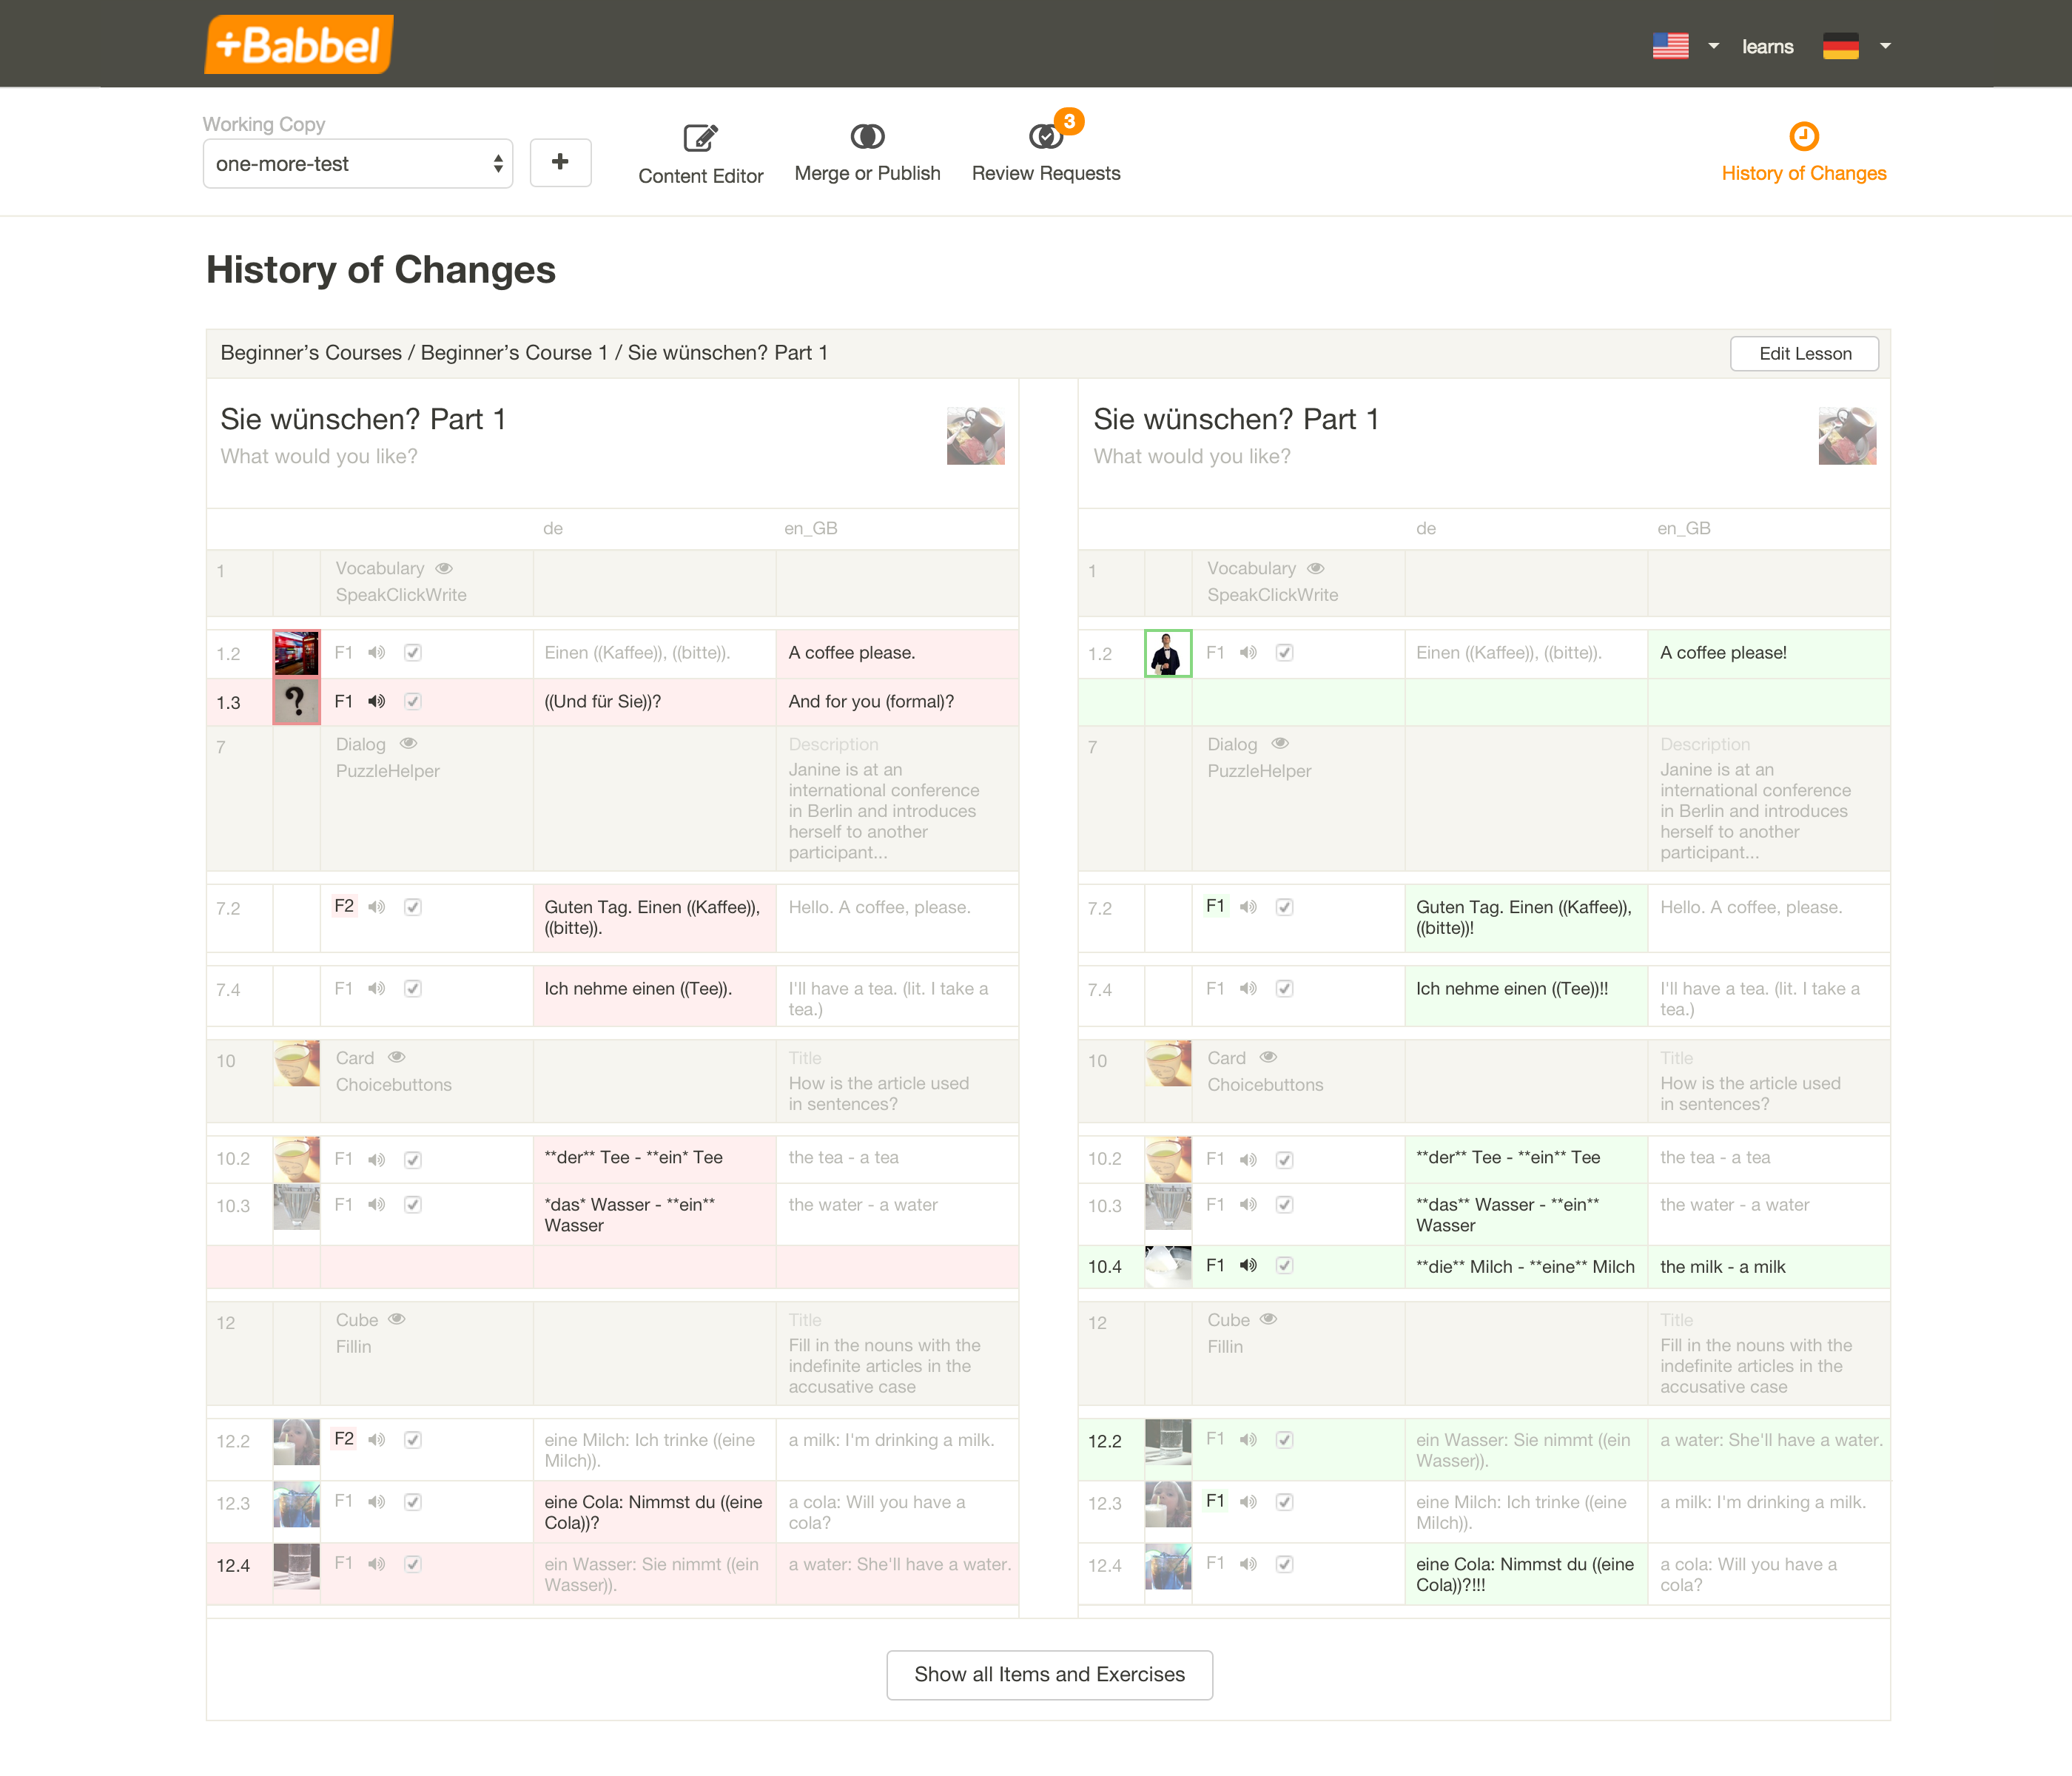
\includegraphics[width=\textwidth]{final-design/diff-split}}
 \caption{Newly designed difference view, which provides more context}
 \label{fig:diff-split}
\end{figure}
% this figure needs to be changed (nav bar is old)

\section{Saving Process}
Saving changes was one of the major pitfalls for users during the last usability study. The redesigned saving process addresses the issues \#41 and \#43 listed in Table \ref{table:issues-saving}. Most of all, users were confused by the existence of two separate saving features (Issue \#41). Even though the saving "shortcut" at the bottom of the editing view was used frequently, it caused confusion when users discovered there is also a second saving button at the top. For this reason, the two separate saving features were combined into one by trying to maintain the advantages of both. The new saving process (Figure \ref{fig:highlighted-changes}) allows users to save their changes on the same page as the edits were done while at the same time giving them the opportunity to review what has changed. The changes are highlighted in green and when hovered reveal the state prior to editing it. Users can decide whether they want to enable this highlighting by toggling a checkbox at the bottom of the view.

Additionally to reducing the steps required to save changes, the new feature also provides better feedback (Issue \#43), because the highlighting disappears after the user saved, signaling that there are no current changes that were not saved yet.

% using two separate saving features wasn't practical. during the user tests it became clear that a global saving function is not needed. whereas in programming it is often necessary to edit several files in order to implement a certain feature in language authroing the editing context is always defined by the immediate surroundings.


\begin{figure}[h!]
 \centering
 \fbox{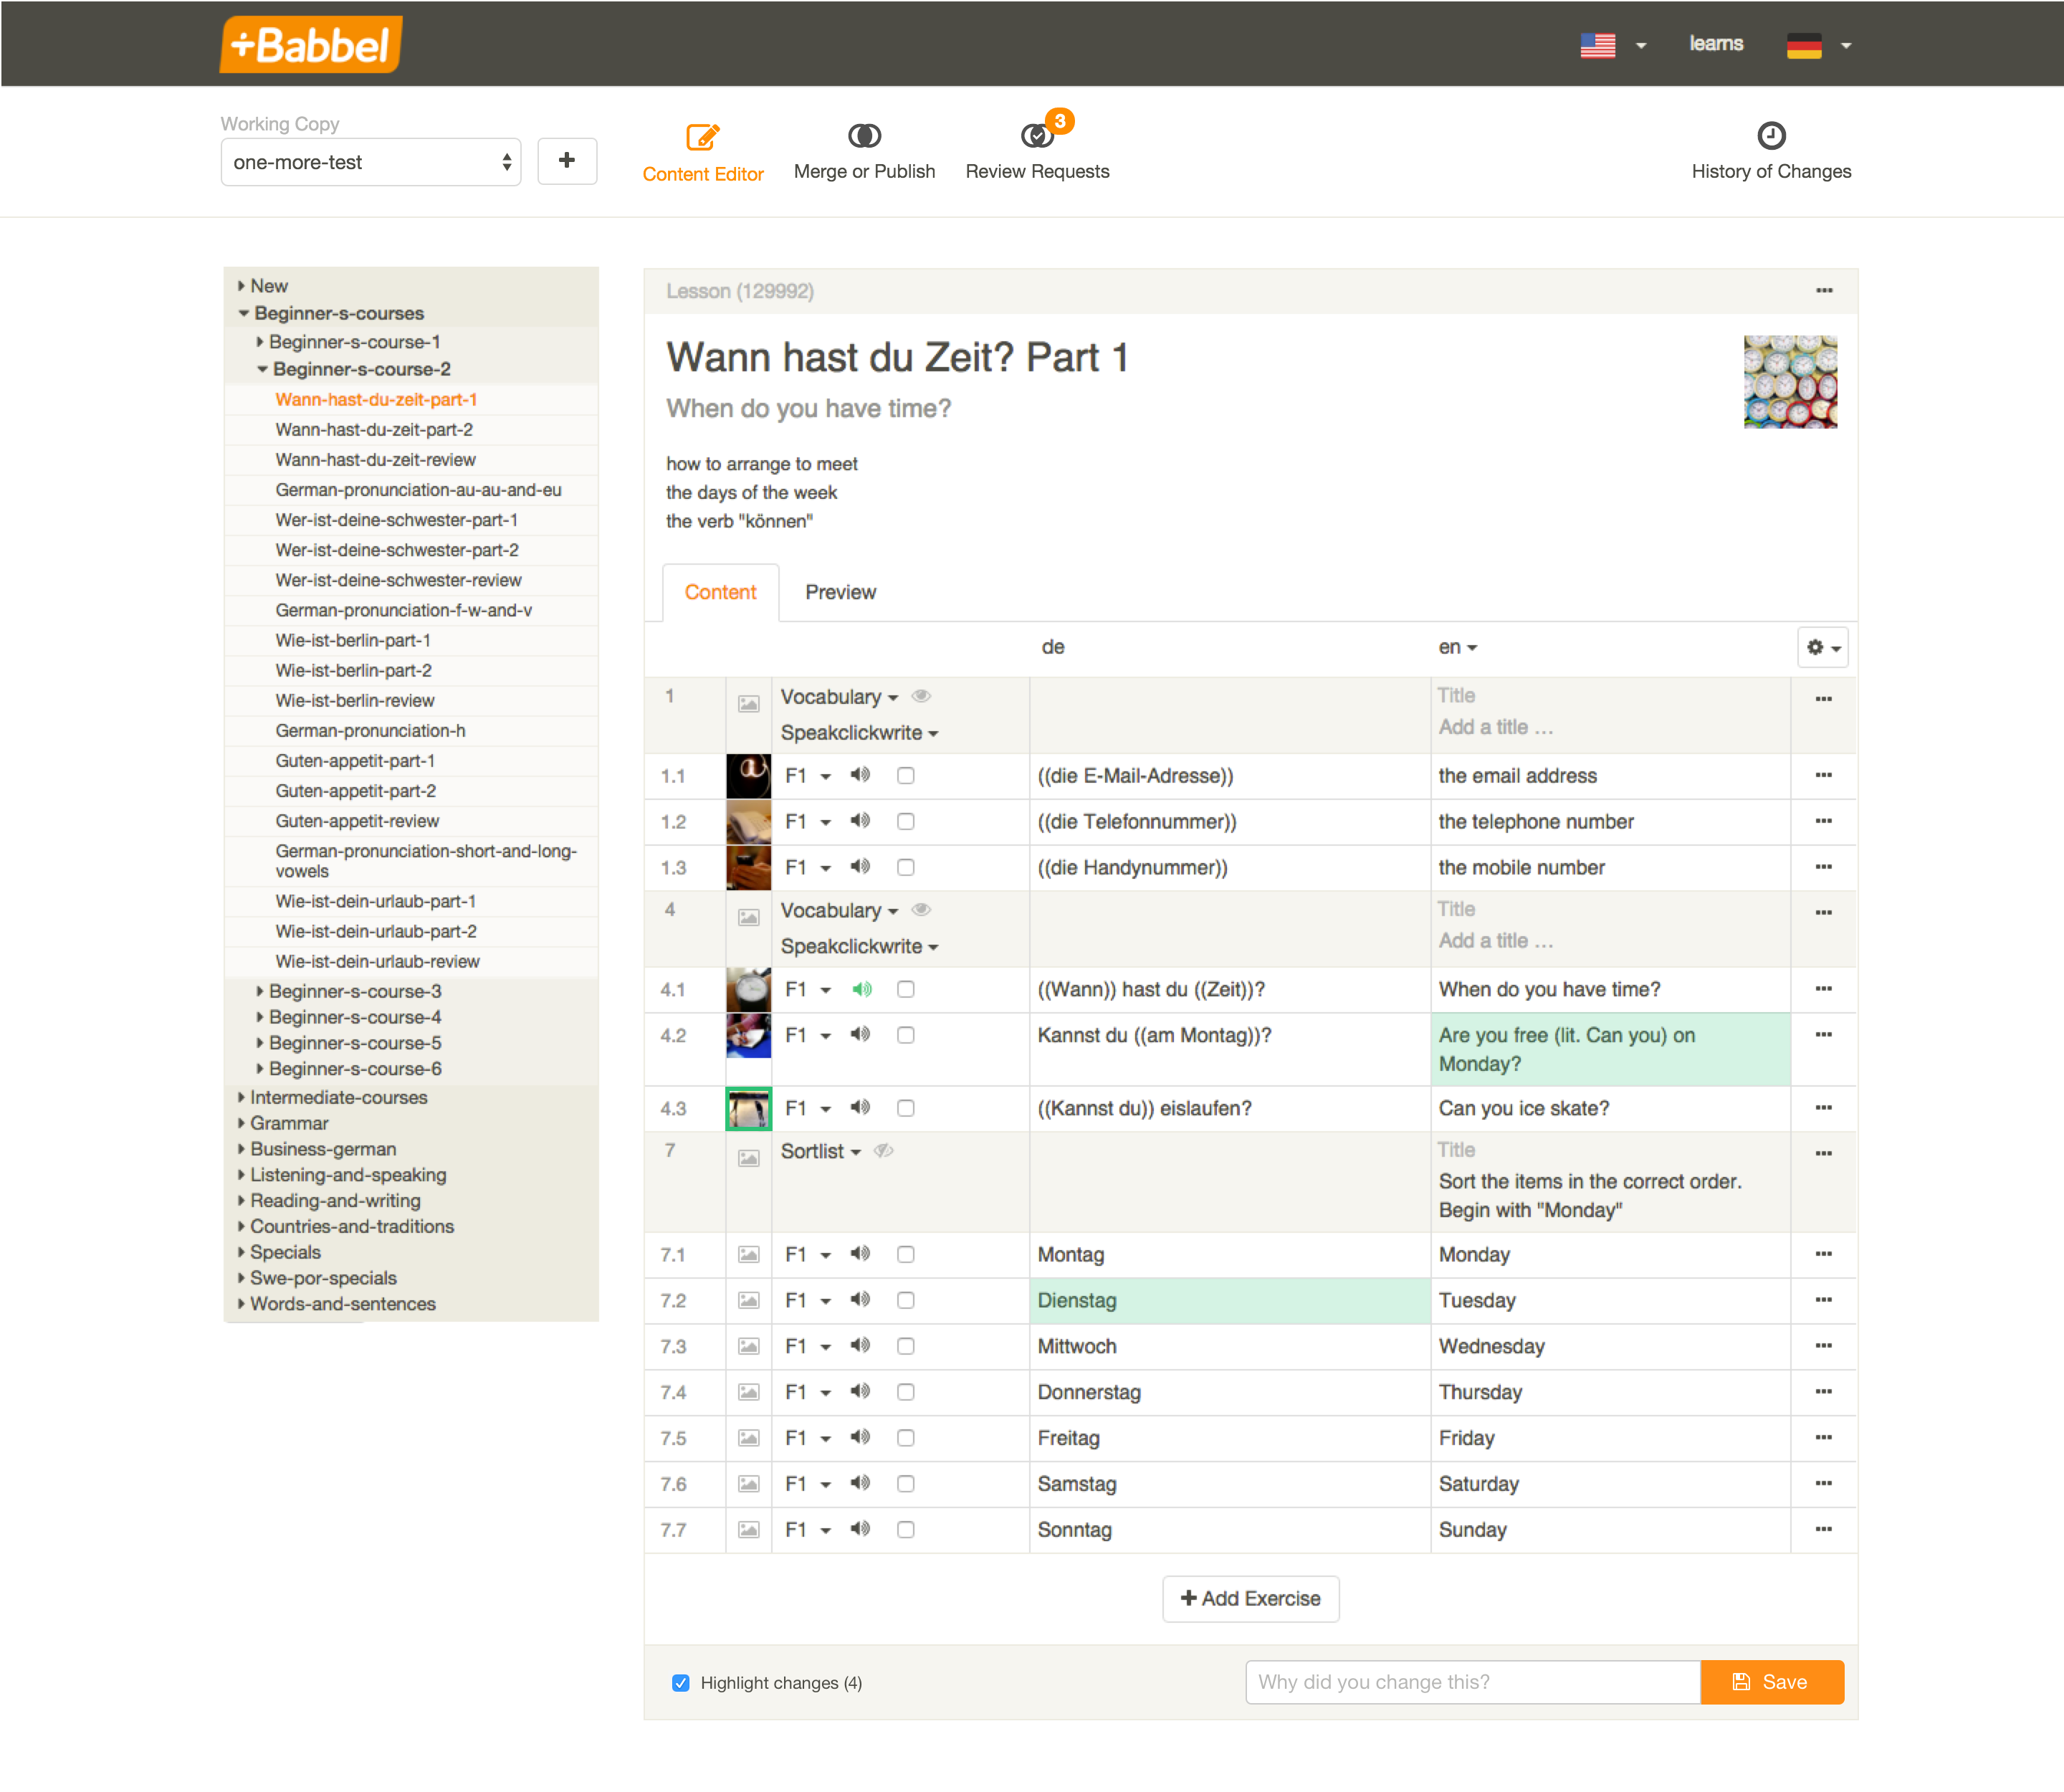
\includegraphics[width=\textwidth]{final-design/edited-highlighting}}
 \caption{The new editing view combines reviewing and saving changes and reduces the amount of clicks needed to save}
 \label{fig:highlighted-changes}
\end{figure}

\begin{figure}[h!]
 \centering
 \fbox{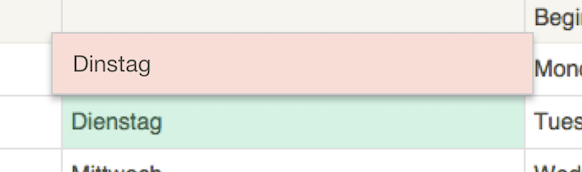
\includegraphics[width=4cm]{final-design/saving-hover-text}}
 \caption{Hovering a highlighted changed exposes the previous value}
 \label{fig:hover-changed-text}
\end{figure}

% \begin{figure}[h!]
%  \centering
%  \fbox{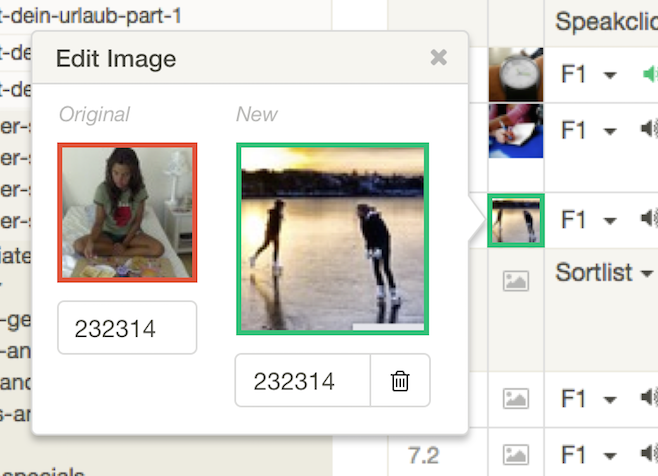
\includegraphics[width=4cm]{final-design/saving-hover-image}}
%  \caption{Hovering a changed image}
%  \label{fig:hover-changed-image}
% \end{figure}


\section{Error Messages}
Another problem that occurred quite frequently during the previous testing sessions were missing or insufficient error messages. Especially during the creation of new working copies, users got stuck, because the interface did not provide appropriate information for recovering from a mistake. The two most common problems where using invalid characters or trying to use a name that was already taken. Now, there are error messages informing users about this (Figure \ref{fig:improv-error-messages}).

Furthermore, the system is more pro-active now. Even though it is technically possible to create an empty merge request, in reality there is no value in doing that. Therefore, the interface now informs users when they are about to do it (Figure \ref{fig:empty-merge-warning}).

\begin{figure}[h!]
 \centering
 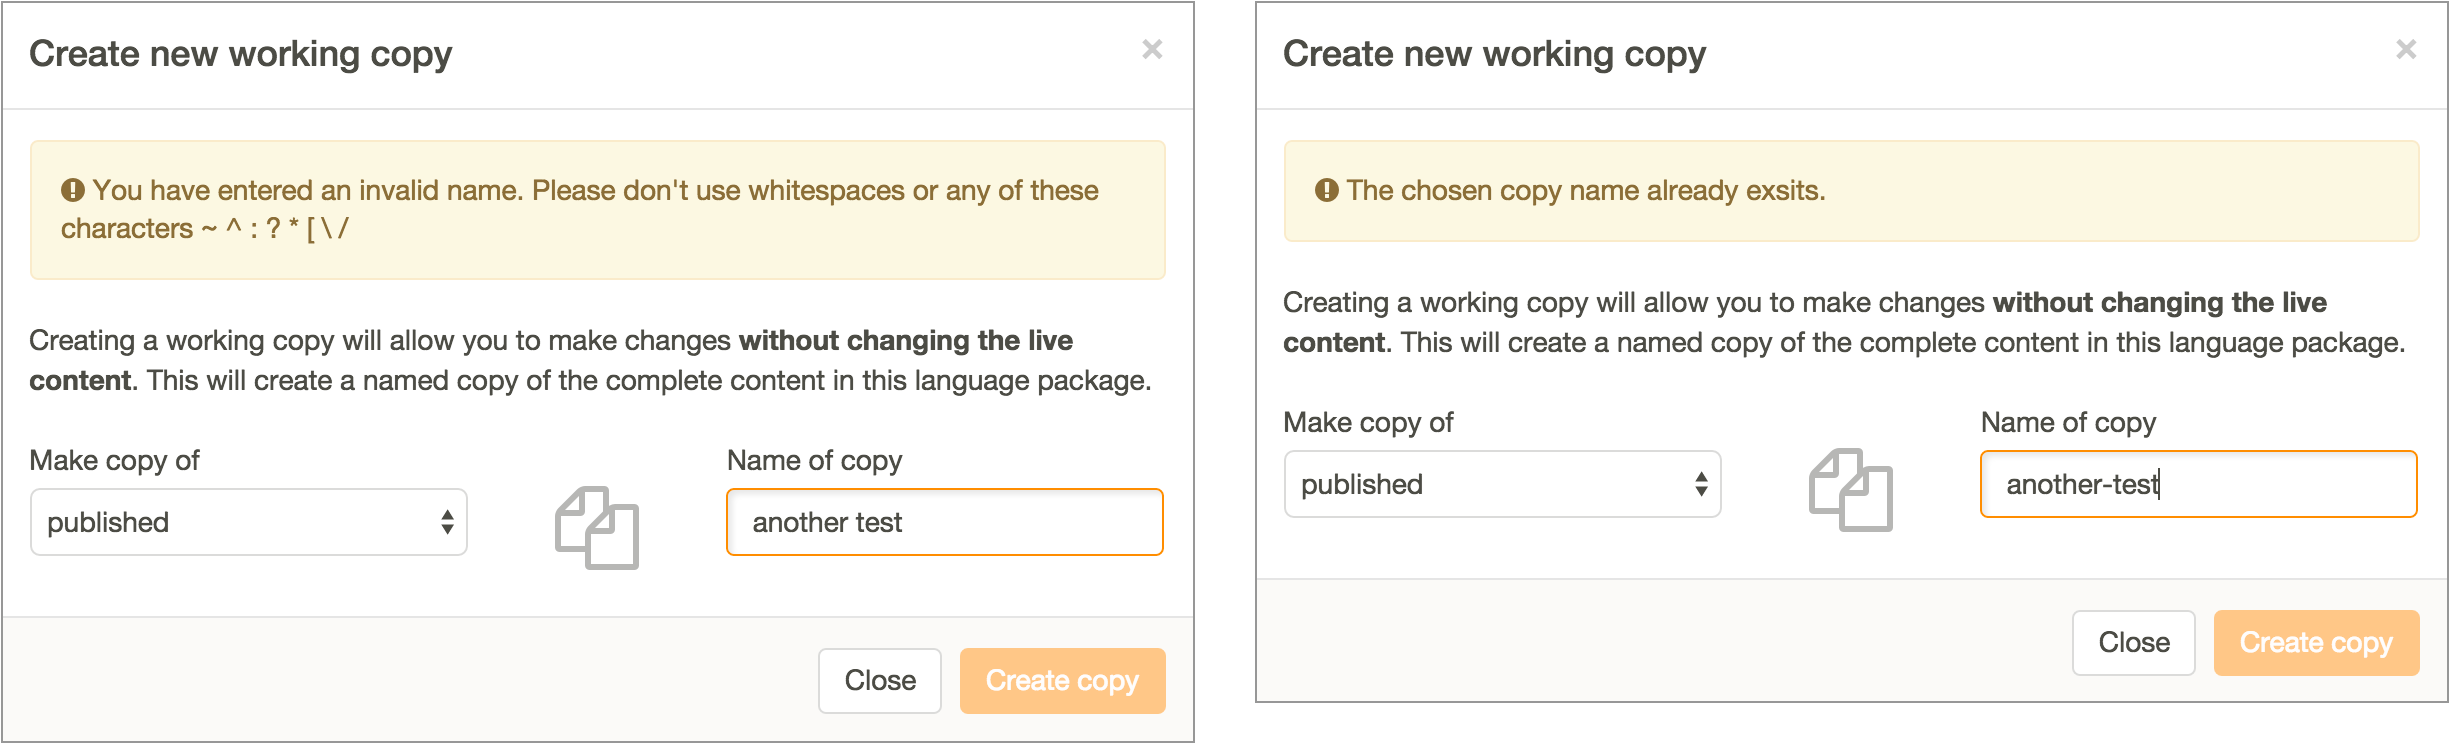
\includegraphics[width=\textwidth]{final-design/error-messages-modal}
 \caption{Improved error message inside working copy modal}
 \label{fig:improv-error-messages}
\end{figure}

\begin{figure}[h!]
 \centering
 \fbox{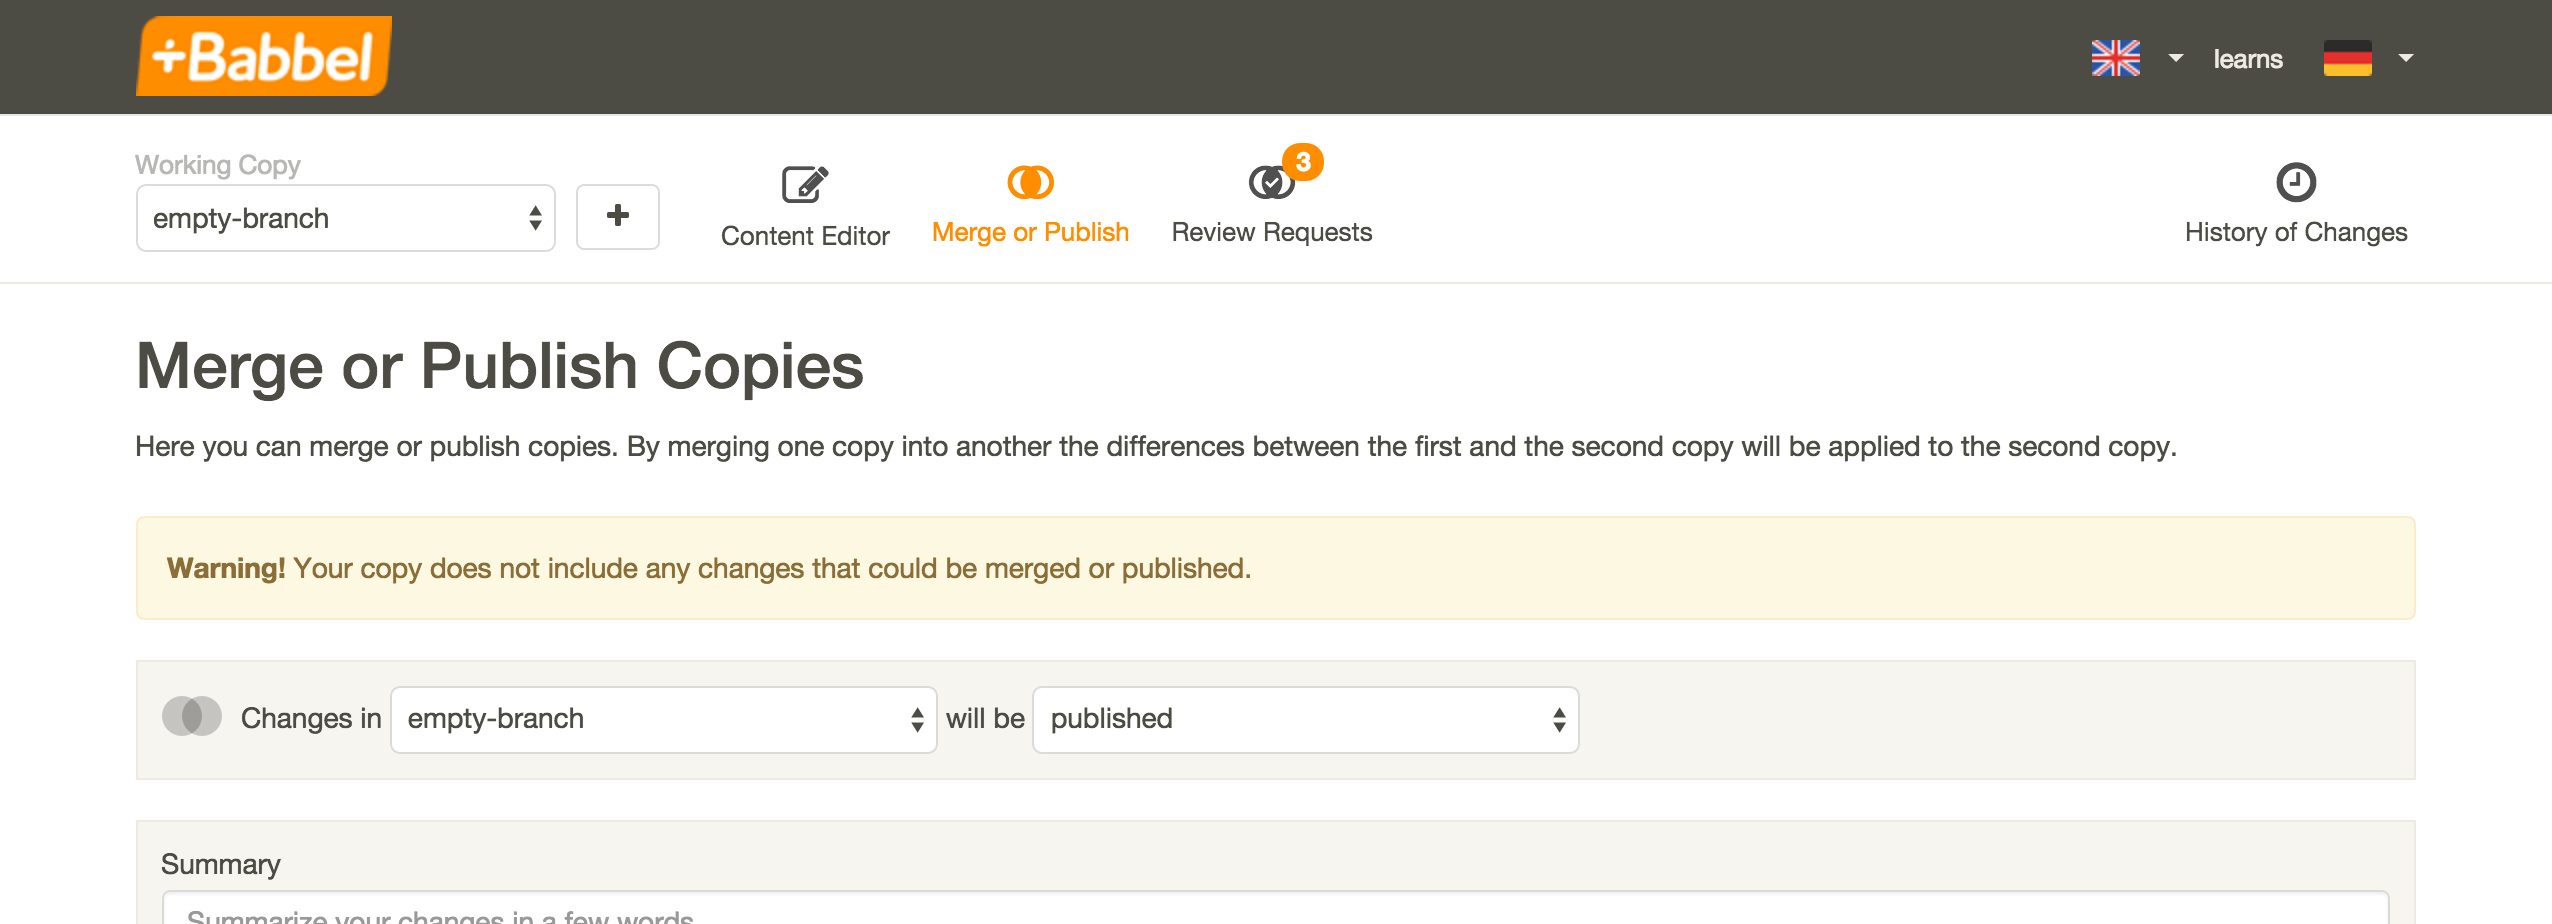
\includegraphics[width=\textwidth]{final-design/empty-merge-warning}}
 \caption{A warning informing users that the selected working copy is equal to the target of the merge}
 \label{fig:empty-merge-warning}
\end{figure}

\section{Navigation Bar}
The top-level navigation was changed conceptually, which also had to be reflected in the layout of the navigation bar (Figure \ref{fig:redesigned-nav}). Instead of treating the different views as "layovers", which were closed with a little \textit{x} in the upper right corner, the navigation now works more like a classical tab-style navigation. Therefore, a new icon for the content editor had to be introduced, which is now placed next to the working copy selection. The "new copy" button was visually grouped with the selection, because these two features conceptually belong together and because it triggered a different behaviour (opening a popup) then the remaining buttons, which result in a complete a view change.

\begin{figure}[h!]
 \centering
 \fbox{
\includegraphics[width=\textwidth]{final-design/new-navigation}}
 \caption{The redesigned navigation bar featuring fewer icons and a consistent way of navigating to the content editor}
 \label{fig:redesigned-nav}
\end{figure}

\section{Miscellaneous Changes}
In order to make the new diff view work, the lesson editing view had to be revised as well. So far, the lesson properties, which include the title, subtitle and a description for every display language, were hidden behind the properties tab. This design was impractical for the new diff view, because everything related to a lesson should be reviewable with just one glance. Therefore, the lesson properties were moved into the header of the editing view and editing was made possible by an inline-editing\footnote{http://ui-patterns.com/patterns/InplaceEditor} solution (Figure \ref{fig:new-lesson-header}). This means that the text turns into an input field when clicked and can be edited.

\begin{figure}[h!]
 \centering
 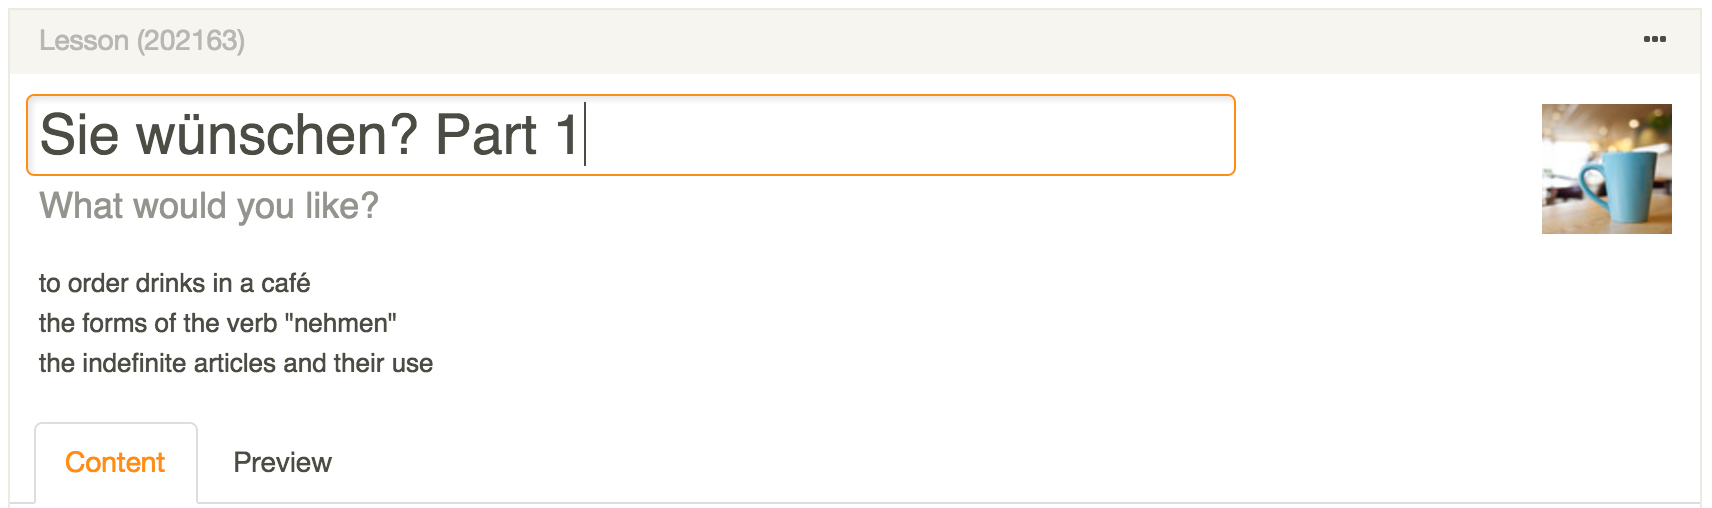
\includegraphics[width=9cm]{final-design/new-lesson-header-editing}
 \caption{New lesson header enabling in-place editing}
 \label{fig:new-lesson-header}
\end{figure}

The new lesson header design described above required another redesign. Now that changing the display language not only affected content that is inside the translation column, but also the text in the lesson header, it seemed odd to select this language in the table header as before. For this reason, the selection was moved to the main navigation bar at the top (Figure \ref{fig:dl-selection}) next to the selection of the learning language.

\begin{figure}[h!]
 \centering
 
\includegraphics[width=4cm]{final-design/dl-selection}
 \caption{Display language selection}
 \label{fig:dl-selection}
\end{figure}

Besides the conceptual changes and those that addressed usability issues directly, a few visual improvements were made in order to reduce the visual clutter. The form for merging or publishing copies was simplified and the input field for the second reviewer is now hidden by default (Figure \ref{fig:merge-publish}). Furthermore, the list of requests (Figure \ref{fig:review-requests}) and the list of changes (Figure \ref{fig:history-of-changes}) were simplified by removing the "show details" button and instead making the whole row clickable. This resulted in less visual clutter and a cleaner interface.

\begin{figure}[h!]
 \centering
 \fbox{\includegraphics[width=\textwidth]{final-design/merge-or-publish}}
 \caption{Merge or publish copies}
 \label{fig:merge-publish}
\end{figure}

\begin{figure}[h!]
 \centering
 \fbox{\includegraphics[width=\textwidth]{final-design/review-requests}}
 \caption{List of requests}
 \label{fig:review-requests}
\end{figure}

\begin{figure}[h!]
 \centering
 \fbox{\includegraphics[width=\textwidth]{final-design/history}}
 \caption{History of changes}
 \label{fig:history-of-changes}
\end{figure}

\chapter{Results and Conclusion} \label{chapter:results-conclusion}
The research question asked in a rather general manner, whether authoring tools can benefit from version control. The thesis at hand tried to answer this question by documenting the user-centered design approach used for designing such a system. The design presented above shows that this it is indeed possible to combine version control and content authoring, but is this liaison beneficial to the tool's users? By looking at the sub-questions first it might become easier to answer the main research question later on.

% specific specific specific, it's the results part after all

\section{Sub-question 1: Feature Reduction and Simplification}
Most version control systems are quite powerful and cover a wide range of use cases. A result of that is a large number of features that come in many different varieties depending on which flag is used and in which context they are used. For example when using Git on the command line the \textit{checkout} command is used for both switching branches as well as creating new ones (using the -b flag). All of this needs to be learned and remembered, which increases the entry barrier for new users. Therefore, one of the questions raised in the beginning was whether certain features could be simplified or eliminated, while still preserving the core functionality of version control. Since the new authoring tool is based on Git, the question was actually, which features to expose to the users and in which way.

The decision which features to expose was based on the requirements and task analysis as well as the literature review. For example, the review has shown that version control users often regard the staging process as laborious and superfluous \cite{perez_de_rosso_whats_2013}. Based on this finding a simpler edit and saving workflow was designed that made staging unnecessary. Additionally, the manual tracking of files was eliminated entirely. As soon as a new content package is created inside the tool it is also tracked by the version control system.

Furthermore, the separation between local and remote repository was eliminated. Users always interact with a remote repository that is stored on Github. Although, this comes with a few disadvantages, such as reduced speed and a single point of failure, overall it simplifies the system and removes hidden dependencies, which Church et al. \cite{church_case_2014} identified as a usability problem. In general, managing repositories is no longer a responsibility of the user, since there is a fixed number of them representing the 14 different learning languages. The user can switch between them, but cannot create new ones or alter them in any way.

% is there more?

The Git reference consists of 53 commands, excluding the low-level features \cite{_gitref_????}. The git command line help still lists 21 "commonly used" commands. Compared to that the interface presented in this section consists of 7 main features related to the version control capabilities. Of course, comparing command line tools with a GUI is not the best way of answering this research question, but it still hints at the reduced complexity.
% count features of Git GUI

%For example the requirements analysis has shown that it is important for users to experiment when creating new content. Therefore, a "work in progress" version is needed that can also be shared among users. %here I'm defending why I introduced a certain feature hmmm

% which features were eliminated?
% how were features simplified

% concurrent editing of the same piece of content

% the requirements showed that users needed to experiment and work



%The biggest insights for tackling this problem were delivered by the literature review.



% talk about no more hidden dependencies
% use term "abstracation barrier" used by church
\section{Sub-question 2: Improve Learnability}
The second sub-question asked how the learnability of the system could be optimized. According to ISO/IEC 9126 \cite{_iso/iec_2001} learnability is a major contributor to a system's usability. As mentioned before, most version control systems, particularly those controlled via command line, require a lot of upfront knowledge about the different commands and  the conceptual model of the system. But, in order to make the authoring tool attractive to a non-technical audience, this complexity should be mostly hidden or exposed only gradually to users. Therefore, a couple of measures were taken to design a system that has a high learnability.

First of all, the initial design was based on insights gained through the literature study and two major studies that investigated the usability of VCSs by Church et al. \cite{church_case_2014} and Jackson and Perez De Rosso \cite{perez_de_rosso_whats_2013}. How these studies influenced the interface design is described in Chapter \ref{chapter:design-first-iteration}.

Secondly, the iterative design process and the user tests ensured that hard to comprehend features were discovered and simplified. Only users with no prior experience in version control software were chosen for the tests (Appendix \ref{append:presession-quest-1}) so that the sessions were a realistic picture of novice users encountering the system for the first time. The outcome of the tests resulted in a couple of design decisions, such as the use of illustrative icons in the navigation bar and warning messages (i.e. for editing live content) that helped users to adopt best practices.

A third and very crucial means of improving the learnability of the system was the focus group that identified terms that were difficult to understand and suggested alternatives. This helped to design an interface which uses terms that are rooted in everyday language rather than one that is comprised of technical jargon.

Of course it is hard to tell whether the implemented version control mechanism is easier to use than one of the many GUI-clients for Git or other version control systems, since the context of use is quite different (code vs. language lessons). But there are a couple of indicators which show that the design of the system has indeed resulted in a good learnability: First of all, the task completion rates for almost all scenarios are quite high (82\% on average during 2nd study). Especially when considering that all participants encountered the system for the first time and basically had to learn it 'on the fly' while performing the tasks, without any introduction or prior tutorial. Additionally, the scores of the post-study questionnaire (Appendix \ref{appendix:pssuq}) for items 5 ("It was easy to learn to use this system" - 2.11) and 6 ("I believe I could become productive quickly using this system." 1.77) show that users are generally happy about the learnability of the system and feel confident to learn it quickly in the future.

% PSSUQ showed that users think they could become efficient quickly using the tool (1.77)
% "I liked using the interface of the system" 1.55
% "The interface of the system was pleasant" 1.66

% some of the questions raised in the beginning can only be answered in the long-term

\section{Sub-question 3: Reducing Initial Overhead}
The third and last research question asked whether the overhead, initially introduced through a version control system, could be reduced. Most version control systems, especially those used in software development, require an additional effort from the user. The reason for this is that instead of just editing and saving files, the user has to administrate repositories, manage branches, define which files should be tracked and describe his or her edits. All this additional effort results in a delayed gratification when the project has increased in size and more and more users are collaborating. But, as is usually the case with delayed gratification, humans are not very good at ignoring small short-term rewards (simpler and faster editing) in favor of greater long-term rewards (file tracking, reversibility, easier collaboration). The challenge therefore was to design a system that reduced the entry barrier as compared to traditional version control systems and helped users to pick up best practices as fast as possible. Was this achieved and if yes how?

The final design offered a couple of solutions to address these issues. First of all, version control comes "pre-installed" with the authoring tool. There is no need to setup repositories or define which files should be tracked. This work "out of the box". Second, users are free to ignore most version control features. If they choose to do so they can just keep on using the authoring tool as they would use other tools without a version control system. Using branches, entering saving descriptions (commit messages) or creating merge requests is entirely optional. Nevertheless, the system tries to teach best practices to the user. When altering public content (master branch) the user is reminded that it is advisable to create a new branch first. If edits are saved without a description, a tooltip explains that a description helps colleagues to better understand why something was changed. Through this mechanisms the user is slowly introduced into version control without the need for him or her to go through an extensive tutorial first. The completion rates (Chapter \ref{chapter:second-iteration}, Figure \ref{table:task-compl}) as well as the relatively low error rates (Chapter \ref{chapter:second-iteration}, Figure \ref{table:second-study-error-rate}), especially during the second study, have shown that it was indeed possible for most users to start using the system without any prior training.

On the other hand there is also room for improvement. The post-study questionnaire had the weakest scores for information quality (3.31), which measures how well the system is documented and how helpful error messages are to the user. This was partially due to the incomplete prototype that was  missing functionality, but nonetheless shows that some users felt there was too little help for using such a system. For those occasions a context-ware help feature could be useful.

Summing up one can say that the overhead of using version control was certainly reduced, but of course not completely eliminated. A system that is more powerful and offers more features will always be harder to learn and use than a simpler system.

% mix of enforcing best practices and offering more complex features optionally - set of minimal features to get started
% overhead was certainly reduced but not eliminated

\section{Conclusion}
Now that we have looked at the sub-questions, let us get back to the main research question. Can authoring tools for e-learning benefit from version control? Ultimately answering this question is difficult, since users have not started using the system in a real-world environment yet. Time will tell whether content authoring really benefits from an integrated version control system. But, what has become clear, is that it is in fact possible to design a version control system that is easier to use and learn than most traditional VCSs and that integrates well with the content authoring process. The system enables users to manage and control the content creation process in ways that were simply not possible before. The authoring tool's capabilities were greatly improved while at the same time increasing the complexity of the tool only moderately. It can be concluded, that version control is indeed a valuable addition to the authoring process of e-learning content and its possible application should be investigated further. The next chapter looks at how this could be done.


% section has shown that it is possible to integrate version control into content authoring, only long term will show whether it is really helpful

% But it is helpful

% documenting the design and thought process of combining these two systems.




% research questions
% main question: Can authoring tools for e-learning benefit from version control?
%\item Which version control features are needed to make the integration useful?
%\item How can the weak learnability of VCSs be improved in order to make the interaction more pleasing for inexperienced users?
%\item How can the overhead, usually introduced through a version control system, be kept to a minimum?

\chapter{Future Work} \label{chapter:future-work}
As mentioned in the previous chapter, the research mostly focused on determining how an easy-to-use interface for version control could be integrated into a content authoring tool. The long-term implications of utilizing such a system were not studied. A possible follow-up study could investigate whether the long-term benefits of the system really outweigh the short-term increase in labour. Furthermore, it should be confirmed which features of the system are actually used and in which way. For this purpose a Web Analytics tool could be used, which would provide more quantitative data and enable a more detailed insight into the usage patterns of the system.

A second area of future research could explore whether the findings of this project also apply to a wider range of tools than just content authoring for e-learning. Given the increasing amount of content created and published online, especially by amateurs, it is conceivable that general purpose systems, such as Wordpress \cite{_wordpress_????} or Drupal \cite{_drupal_????} could benefit from this as well. In order to find out, more research would be needed in regards to the ability of occasional users to learn and remember such a system.

Summing up, one could say, that the expansion of version control outside of software development is a recent development, which has slowly shifted the focus to usability and simpler interfaces. Probably, there are more use cases for these systems than the current research landscape suggests. If the HCI community continues to prove, that version control is also viable outside a purely technical domain, it might increasingly appear inside more mainstream products in the future.




% 1. How could the presentated research be improved if it were repeated?

%make long-term study and compare to existing/old content authoring tool to see how much it is used and whether it is appreciated

% 2. What would be the appropriate question(s) for future research starting from what is presented here?


% https://guidetogradschoolsurvival.wordpress.com/2011/04/15/how-to-write-future-workconclusions-2/

% What do you think are the next steps to take?
% What other questions do your results raise?
% Do you think certain paths seem to be more promising than others?

% Another way to look at the future work section, is a way to sort of “claim” an area of research. This is not to say that others can’t research the same things, but if your paper gets published, it’s out there that you had the idea.

% it has been proven that version control can be a useful addition to tools not related to programming.
% a first step has been made in bringing version control to a wider audience. the thesis has shown that VCSs can be useful for content authoring, but it is easy to imagine that content management systems could benefit from this as well.

% merge conflicts were not covered - no solution yet

% Questions to ask:
% 1. How could the presentated research be improved if it were repeated?
% 2. What would be the appropriate question(s) for future research starting from what is presented here?


\cleardoublepage %to make sure that the first page number for the references is correctly listed in the TOC.
\addcontentsline{toc}{chapter}{References}
\bibliographystyle{IEEEtran}
\bibliography{IEEEfull,Mybibliography}


\noappendicestocpagenum
\addappheadtotoc

\begin{appendix}

%\include{appendix_A}
\chapter{Background of First User Study} 
\label{sec:first-iteration-scenarios}

%Anything that does not directly contribute to the understanding for the reader, but is still relevant in order to support particular claims made in the report (for instance a purely mathematical derivation), should be put in the appendix. (That is, only if it cannot be found elsewhere. Otherwise a simple citation suffices.)

%For the rest the appendices are like the other chapters, i.e. they can have sections, figures, tables, and citations (even though the appendix comes after the list of references).

\section{Scenarios}
The following task scenarios were given to participants of the first iteration user studies. The link leads to the original prototype that was used.

\subsection{Scenario 1}
\begin{itemize}
  \item End goal: Let colleague review changes
  \item Estimated time: 8 mins
  \item Link: https://marvelapp.com/c89590
\end{itemize}

A colleague (Firstname Lastname) has sent you a link to a lesson.
She informed you that the second item in the vocabulary (write) exercise has the wrong speaker role (should be F1) and also should be added to the review manager. 
She asked you to correct the error and afterwards allow her to review your changes. 
Make sure you’re not editing the live content.

\subsection{Scenario 2}
\begin{itemize}
  \item End goal: Publishing changed content
  \item Estimated time: 4 mins
  \item Link: https://marvelapp.com/1011fjj
\end{itemize}

A colleague (Firstname Lastname) has changed a lesson within the German language package.
She asked you to review the changes. 
Look at the changes she made and if you don’t find any errors make them available to the Babbel end-user.

\subsection{Scenario 3}
\begin{itemize}
  \item End goal: Eliminating error and save
  \item Estimated time: 6 mins
  \item Link: https://marvelapp.com/102f4b4
\end{itemize}

A translator (user name: rcarlos) is currently working on a localization of German lessons (to Portuguese). 
Recently a translated exercise was published, but according to customer service users have complained that there is a translation missing within this exercise. 
Find the exercise which has been translated and locate the item with the missing translation. 
Add the translation and save your changes.

\section{Pre-session Questionnaire} \label{append:presession-quest-1}

\begin{table}[h!]
\begin{tabular}{|l|p{3cm}|p{1.5cm}|p{2cm}|p{3cm}|}
\hline
{\bf User} & {\bf Familiar with version control?} & {\bf Used it?} & {\bf Experience with current tool} & {\bf Used other content management or authoring systems?} \\ \hline
1                 & No                                        & No                       & 1 - 3 years                        &                                                        \\ \hline
2                 & No                                        & No                       & 1 - 3 years                        &                                                        \\ \hline
3                 & No                                        & No                       & 3 months - 1 year                  & WordPress                                              \\ \hline
4                 & No                                        & No                       & more than 3 years                  &                                                        \\ \hline
5                 & No                                        & No                       & 1 - 3 years                        &                                                        \\ \hline
\end{tabular}
\centering
\caption{Pre-session questionnaire}
\label{table:pre-sess-quest}
\end{table}
\chapter{Background of Second User Study}

% \section{Participant Quotes} \label{appendix:quotes}

% \subsection{Working Copies}

% \begin{itemize}
%  \item "Am I in the copy right now?"
%  \item "I have created a copy but I'm not sure whether I have selected it"
% \end{itemize}

% \subsection{Saving Process}

% \begin{itemize}
%  \item "Why do I have to answer why?"
%  \item "No unsaved changes?" (related to blank slate)
% \end{itemize}

% \subsection{Merge Requests}

% \begin{itemize}
%  \item "I think I didn't read the text properly because I don’t really get what merge and publish means"
%  \item "The merge and publish is confusing me"
%  \item "It would be easier if you had it straight after the save changes"
%  \item "I don't see what is addressed to me" (list of requests)
% \end{itemize}

% \subsection{Navigation}

% \begin{itemize}
%  \item "If I wanna go back can I close this?"
% \end{itemize}

\section{Pre-session Questionnaire}

\begin{table}[h!]
\centering
\begin{tabular}{|l|p{3.5cm}|p{1.5cm}|p{3.5cm}|p{3.5cm}|}
\hline
\rowcolor[HTML]{EFEFEF}
\textbf{User} & \textbf{Familiar with VCSs} & \textbf{Used VCS} & \textbf{Experience with current tool} & \textbf{Other CMS or authoring tools} \\ \hline
1 & Yes & No & Less than 3 months &  \\ \hline
2 & No & No & 1 - 3 years & Wordpress \\ \hline
3 & Yes & No & 1 - 3 years &  \\ \hline
4 & No & No & 1 - 3 years &  \\ \hline
5 & No & No & more than 3 years &  \\ \hline
6 & No & No & more than 3 years & Drupal, Adobe E-Learning Tool and iBooks \\ \hline
7 & No & No & 1 - 3 years &  \\ \hline
8 & No & No & Less than 3 months &  \\ \hline
9 & No & No & 1 - 3 years &  \\ \hline
10 & No & No & Less than 3 months & WordPress, Imperia 8 \\ \hline
\end{tabular}
\caption{Pre-session questionnaire of second user study}
\label{table:pre-sess-quest-second}
\end{table}

\section{Average Scores for 16 PSSUQ Items} \label{appendix:pssuq}

\begin{table}[h!]
\centering
\begin{tabular}{|l|p{8cm}|r|}
\hline
\rowcolor[HTML]{EFEFEF}
\# & {\bf Item} & {\bf Rating} \\ \hline
1 & Overall, I am satisfied with how easy it is to use this system. & 2.55 \\ \hline
2 & It was simple to use this system. & 3.00 \\ \hline
3 & I was able to complete the tasks and scenarios quickly using this system. & 3.44 \\ \hline
4 & I felt comfortable using this system. & 2.22 \\ \hline
5 & It was easy to learn to use this system. & 2.11 \\ \hline
6 & I believe I could become productive quickly using this system. & 1.77 \\ \hline
7 & The system gave error messages that clearly told me how to fix problems. & 3.77 \\ \hline
8 & Whenever I made a mistake using the system, I could recover easily and quickly. & 3.11 \\ \hline
9 & The information (such as online help, on-screen messages and other documentation) provided with this system was clear. & 3.33 \\ \hline
10 & It was easy to find the information I needed. & 3.55 \\ \hline
11 & The information was effective in helping me complete the tasks and scenarios. & 3.11 \\ \hline
12 & The organization of information on the system screens was clear. & 3.00 \\ \hline
13 & The interface of this system was pleasant. & 1.66 \\ \hline
14 & I liked using the interface of this system. & 1.55 \\ \hline
15 & This system has all the functions and capabilities I expect it to have. & 3.00 \\ \hline
16 & Overall, I am satisfied with this system. & 2.11 \\ \hline
\end{tabular}
\caption{All 16 items of the PSSUQ}
\label{table:pssuq-items}
\end{table}


\end{appendix}


\end{document}
